\documentclass[letterpaper, 12pt]{article}
\usepackage[french]{babel}

\usepackage{amsmath,amsfonts,amsthm,amssymb,graphicx,wasysym,multirow}
\usepackage[latin1]{inputenc}

\usepackage{hyperref}

\pagestyle{plain}

\setlength{\topmargin}{-2cm}
\setlength{\textheight}{23.5cm}
\setlength{\textwidth}{18cm}
\setlength{\oddsidemargin}{-1cm}
\setlength{\parindent}{0pt}

\begin{document}

3000-- Les \'Egyptiens ne savaient qu'additionner et multiplier par 2. Ils utilisaient les symboles suivants pour faire leurs calculs.\\

\begin{center}
\begin{tabular}{|c|c|c|}
\multicolumn{3}{c}{\bf Symboles \'egyptiens}\\[2mm] \hline
{\bf Symbole} & {\bf Signification} & {\bf Nombre}  \\ \hline \hline
 & & \\
\includegraphics[scale=0.8]{Hiero1.eps} & b\^aton & 1\\[4mm] \hline
 & & \\
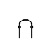
\includegraphics[scale=1.6]{Hiero10.eps} & anse de panier & 10\\[4mm] \hline
 & & \\
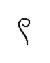
\includegraphics[scale=1.5]{Hiero100.eps} & rouleau de Papyrus & 100\\[4mm] \hline
 & & \\
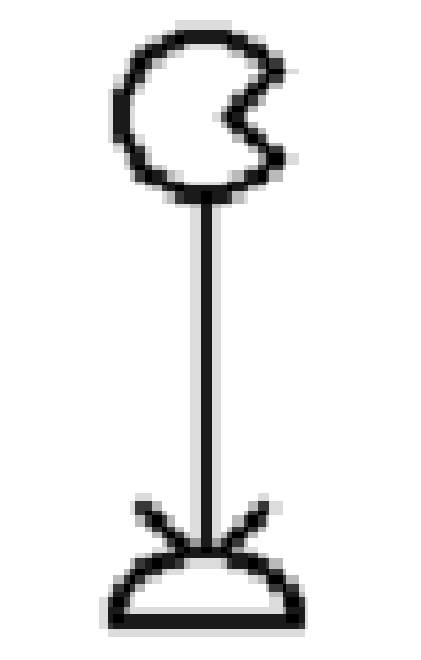
\includegraphics[scale=0.08]{Hiero1000.eps} & fleur de lotus & 1000\\[4mm] \hline
\multicolumn{3}{c}{}\\
\end{tabular}
\end{center}

\`A l'aide du tableau, calculer la somme suivante :
\begin{center}
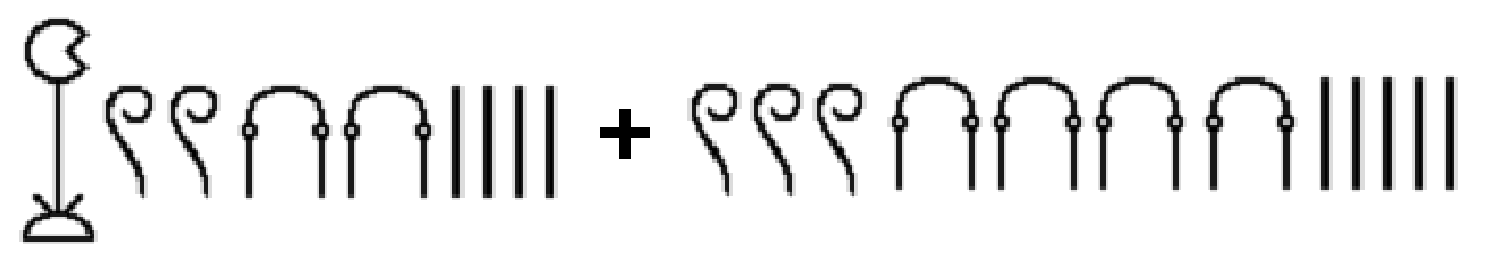
\includegraphics[scale=0.35]{1569.eps}\\
\end{center}

R\'eponse : $1569$\\

R\'etroaction :\\
La fleur de lotus vaut $1000$, le rouleau de Papyrus $100$, l'anse de panier $10$ et le b\^aton $1$.\\
Donc, le premier groupe de symbole:\\
\begin{center}
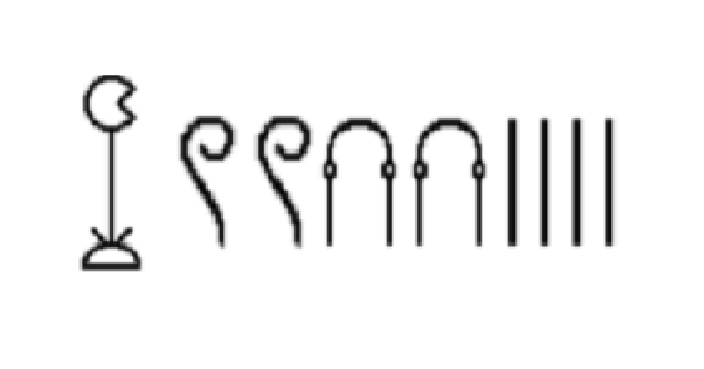
\includegraphics[scale=0.35]{1224.eps}\\
$= 1000 + 2 \times 100 + 2 \times 10 + 4 \times 1 = 1224$.\\[4mm]
\end{center}
Et le deuxi\`eme:\\
\begin{center}
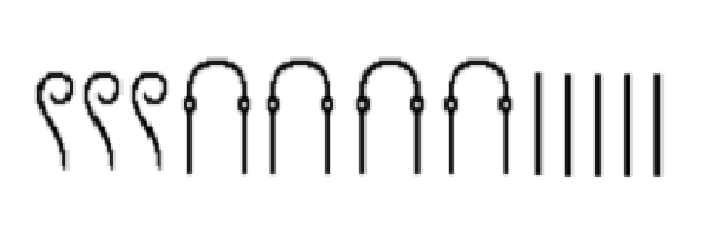
\includegraphics[scale=0.35]{345.eps}\\
$= 3 \times 100 + 4 \times 10 + 5 \times 1  = 345$.\\[4mm]
\end{center}
Donc la r\'eponse est : $1224 + 345 = 1569$.\\

Images prises sur le site : \href{http://fr.wikipedia.org/wiki/Num\%C3\%A9ration \%C3\%A9gyptienne}{fr.wikipedia.org/wiki/Num\'eration \'egyptienne}\\



3001-- Parmi les symboles suivants, lequel repr\'esente un nombre \'ecrit en babylonien?\\


a) :\textsf{P}\\
b) XXIV\\
c) 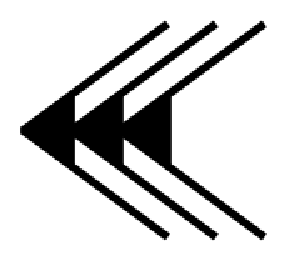
\includegraphics[scale=0.1]{30.eps} \includegraphics[scale=0.1]{5.eps}\\
d) 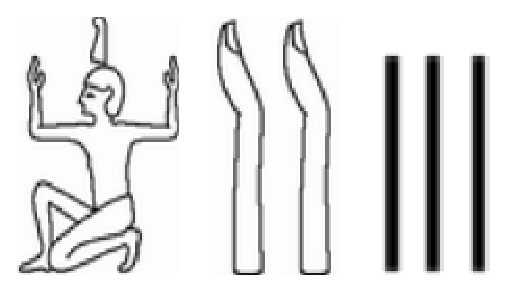
\includegraphics[scale=0.15]{nombregyptien.eps}\\

R\'eponse : c)\\

R\'etroaction :\\
:\textsf{P} est une grimace dans le langage du clavardage.\\
XXIV est le nombre $24$ en chiffres romains.\\
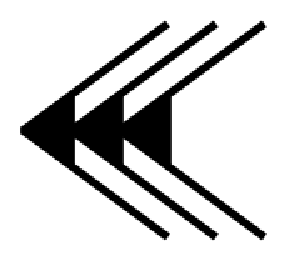
\includegraphics[scale=0.1]{30.eps} \includegraphics[scale=0.1]{5.eps} est le nombre 35 en \'ecriture babylonienne.\\
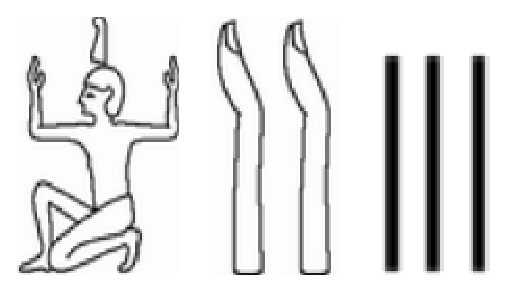
\includegraphics[scale=0.12]{nombregyptien.eps} est le nombre 1 020 003 en \'ecriture \'egyptienne.\\
La r\'eponse est donc c).\\

Images prises sur le site : \href{http://fr.wikipedia.org}{fr.wikipedia.org}\\



%{\bf \textsf{animation : bonhomme d\'eguis\'e en romain appara\^it, poings sur les hanches, chevelure au vent}}\\
3002-- Que vaut le nombre romain suivant: MMCDLXIV ?\\

a) $2464$\\
b) $2666$\\
c) $5444$\\
d) $5466$\\

R\'eponse : a)\\

R\'etroaction :\\
\begin{center}
\begin{tabular}{|c|c|}
\multicolumn{2}{c}{\bf Liste des chiffres}\\[2mm] \hline
{\bf Chiffres Romains} & {\bf Nombres} \\[1mm] \hline \hline
M & 1000 \\[1mm] \hline
D & 500 \\[1mm] \hline
C & 100 \\[1mm] \hline
L & 50 \\[1mm] \hline
X & 10 \\[1mm] \hline
V & 5 \\[1mm] \hline
I & 1 \\[1mm] \hline
\multicolumn{2}{c}{}\\
\end{tabular}
\end{center}
Pour former un nombre, on \'ecrit chaque lettre en ordre d\'ecroissant de leur valeur. Par exemple, on \'ecrit MI pour $1001$. On additionne les valeurs de chaque lettre pour former le nombre, sauf si
\begin{center}
I est \`a gauche de V ou X,\\
X est \`a gauche de L ou C,\\
C est \`a gauche de D ou M.\\
\end{center}
Dans ce cas, on soustrait la lettre \`a gauche (par exemple: XL = L -- X = $50 - 10 = 40$).\\

Donc, MMCDLXIV = $1000 + 1000 + (500 - 100) + 50 + 10 + (5 - 1) = 2464$. La r\'eponse est a).\\



%{\bf\textsf{animation : le petit bonhomme compte ses doigts}}\\
3003-- Les chiffres \og $0, 1, 2, 3, 4, 5, 6, 7, 8, 9$ \fg \ sont d'origine arabe. Pourquoi les Arabes ont d\'ecid\'e d'utiliser le syst\`eme d\'ecimal (en base 10) pour faire des math\'ematiques ?\\

a) Chaque Arabe poss\'edait 10 moutons.\\
b) 10 \'etait un nombre religieux sacr\'e.\\
c) L'homme a 10 doigts.\\
d) La famille royale \'etait constitu\'ee de 10 enfants \`a l'\'epoque.\\

R\'eponse : c)\\

R\'etroaction :\\
Tout porte \`a croire que le syst\`eme d\'ecimal vient de la possibilit\'e de compter sur nos dix doigts. En anglais, les chiffres sont appel\'es \og digits \fg, du mot latin \og digitus \fg \ qui veut dire doigt. La r\'eponse est donc c).\\



3004-- Quand a-t-on utilis\'e pour la premi\`ere fois des symboles arithm\'etiques pour faire des math\'ematiques ? (par exemple: $+, -, \times , \leq , \geq $)\\

a) durant la Pr\'ehistoire\\
b) $1000$ ans avant J\'esus-Christ, \`a l'\'epoque babylonienne\\
c) au {\scriptsize XIV\ieme{}} si\`ecle, au d\'ebut de la Renaissance\\
d) au {\scriptsize XX\ieme{}} si\`ecle\\

R\'eponse : c)\\

R\'etroaction :\\
\`A l'\'epoque de la Gr\`ece antique et avant, il n'existait pas de symbole pour les op\'erations et les relations arithm\'etiques. Les gens \'ecrivaient tous leurs probl\`emes et leurs solutions en mots. Ce n'est qu'au d\'ebut de la Renaissance que l'on voit appara\^itre les premiers symboles \'ecrits \`a la main. Donc, la r\'eponse est c).\\



3005-- Combien existe-t-il de symboles diff\'erents pour repr\'esenter la multiplication ?\\

a) 1\\
b) 2\\
c) 3\\
d) 4\\

R\'eponse: d)\\

R\'etroaction :\\
\begin{center}
\begin{tabular}{|l|c|c|}
\multicolumn{3}{c}{\bf \'Evolution du symbole de multiplication}\\[2mm] \hline
{\bf Date d'apparition} & {\bf Symbole} & {\bf Exemple} \\[1mm] \hline \hline
{\scriptsize IX\ieme{}} si\`ecle & juxtaposition & $3 \, (4 + 5)$ \\[1mm] \hline
d\'ebut {\scriptsize XVII\ieme{}} si\`ecle & $\times$ & $3 \times (4 + 5)$ \\[1mm] \hline
1698 & $\cdot$ & $3 \cdot (4 + 5)$ \\[1mm] \hline
aujourd'hui (plus courant en langage informatique) & $\ast$ & $3 \ast (4 + 5)$ \\[1mm] \hline
\multicolumn{3}{c}{}
\end{tabular}
\end{center}
Le symbole $\cdot$ est apparu, car les math\'ematiciens de l'\'epoque craignaient qu'il y ait confusion entre le symbole $\times$ et la variable $x$. Il y a donc quatre symboles pour repr\'esenter la multiplication. La r\'eponse est d).\\



3006-- Combien existe-t-il de symboles diff\'erents pour repr\'esenter la division ?\\

a) 1\\
b) 2\\
c) 3\\
d) 4\\

R\'eponse: d)\\

R\'etroaction :\\
\begin{center}
\begin{tabular}{|c|c|l|}
\multicolumn{3}{c}{\bf \'Evolution du symbole de division}\\[2mm] \hline
{\bf Symbole} & {\bf Exemple} & {\bf Notes} \\ \hline \hline
$\div$ & $3 \div 5$ & paru pour la premi\`ere fois dans un livre Suisse au 17\ieme{} si\`ecle \\[1mm] \hline
$/$ & $3 / 5$ & premi\`ere fa\c con d'\'ecrire une fraction\\[1mm] \hline
$-$ & $\frac{3}{5}$ & autre fa\c con d'\'ecrire la fraction \\[1mm] \hline
$:$ & $3:5$ & ratio \\[1mm] \hline
\multicolumn{3}{c}{}
\end{tabular}
\end{center}
Il y a donc quatre fa\c cons d'\'ecrire le symbole de la division. La r\'eponse est d).\\



3007-- Quelle d\'ecouverte math\'ematique importante utilisons-nous tous les jours, mais qui, \`a l'\'epoque, \'etait difficile \`a comprendre?\\

a) compter sur ses doigts\\
b) l'addition\\
c) la g\'eom\'etrie\\
d) le z\'ero\\

R\'eponse : d)\\

R\'etroaction :\\
Bien que toutes ces d\'ecouvertes soient importantes, l'une d'elles \'etait plus difficile \`a comprendre.\\
Au {\scriptsize IX\ieme{}} si\`ecle, les Indiens ont d\'efini un concept math\'ematique important, le \og \emph{z\'ero} \fg. Comme la plupart du temps, les nombres ne servaient qu'\`a compter des objets, il \'etait difficile d'associer le concept \og il n'y a pas d'objet \fg \ (donc il n'y a rien \`a compter) \`a un nombre. Ils ont d'abord d\^u voir les chiffres $1, 2, 3, ...$ comme des objets et non seulement comme des adjectifs num\'eraux. Par la suite, ces chiffres devaient exister m\^eme s'il n'y avait rien \`a compter. Et seulement l\`a, l'id\'ee du z\'ero a pu na\^itre. La r\'eponse est donc d). C'est le math\'ematicien Al-Khwarizmi qui a transmis cette id\'ee du z\'ero \`a l'Ouest Europ\'een.
\begin{center}
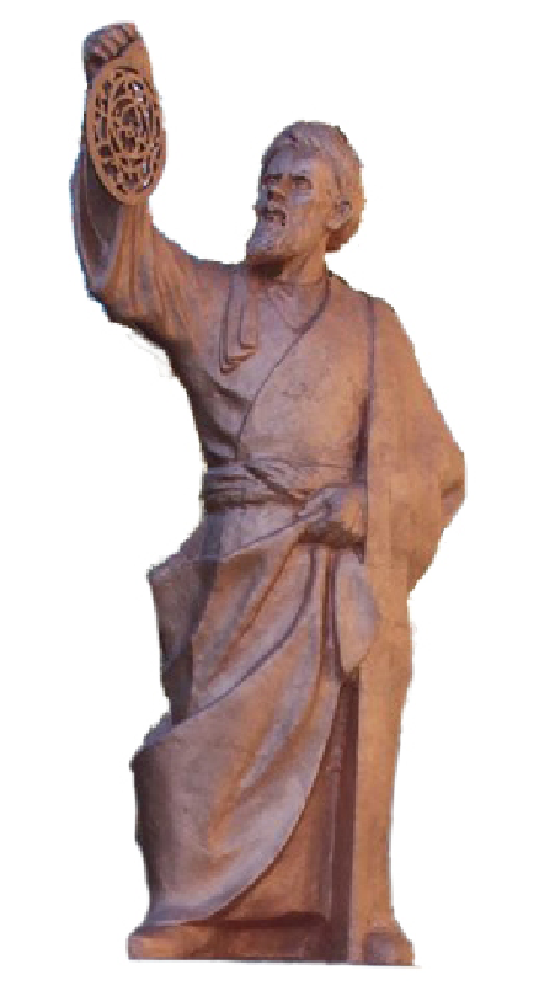
\includegraphics[scale=0.25]{Al-Khwarizmi.eps}\\
\emph{{\small Al-Khwarizmi}}\\
\href{http://fr.wikipedia.org/wiki/Al-Khwarizmi}{fr.wikipedia.org/wiki/Al-Khwarizmi}\\[5mm]
\end{center}



3008-- Au {\scriptsize XVII\ieme{}} si\`ecle, on a propos\'e de r\'esoudre une \'equation de degr\'e 2 de la fa\c con suivante: \og \emph{D\'eplacer tous les termes du m\^eme c\^ot\'e de l'\'egalit\'e de telle sorte qu'elle soit \'egale \`a z\'ero.} \fg
\begin{eqnarray*}
x^{2} + 2 &=& 3x\\
x^{2} - 3x +2 &=& 0
\end{eqnarray*}\\
\og \emph{Factoriser et poser chaque facteur \'egal \`a z\'ero.} \fg
\begin{eqnarray*}
x^{2} - x - 2x +2 = 0\\
x\cdot(x - 1) - 2\cdot(x - 1) = 0\\
(x - 1)\cdot(x - 2) = 0\\
(x - 1) = 0 \ \ \textrm{et} \ \ (x - 2) = 0\\
x = 1 \ \ \textrm{et} \ \ x = 2
\end{eqnarray*}\\
Quel math\'ematicien anglais a eu cette id\'ee?\\

a) Andre\"i Markov\\
b) John Pell\\
c) Thomas Harriot\\
d) Z\'enodore\\

R\'eponse : c)\\

R\'etroaction :\\
Andre\"i Markov est le nom d'un math\'ematicien russe et d'un joueur de hockey russe. John Pell est un math\'ematicien anglais qui est connu pour l'\'equation de Pell. C'est Thomas Harriot qui a \'enonc\'e cette id\'ee pour r\'esoudre les \'equations de degr\'e 2. On appelle parfois ce principe \og \emph{le principe d'Harriot} \fg. Donc, la r\'eponse est c).\\
\begin{center}
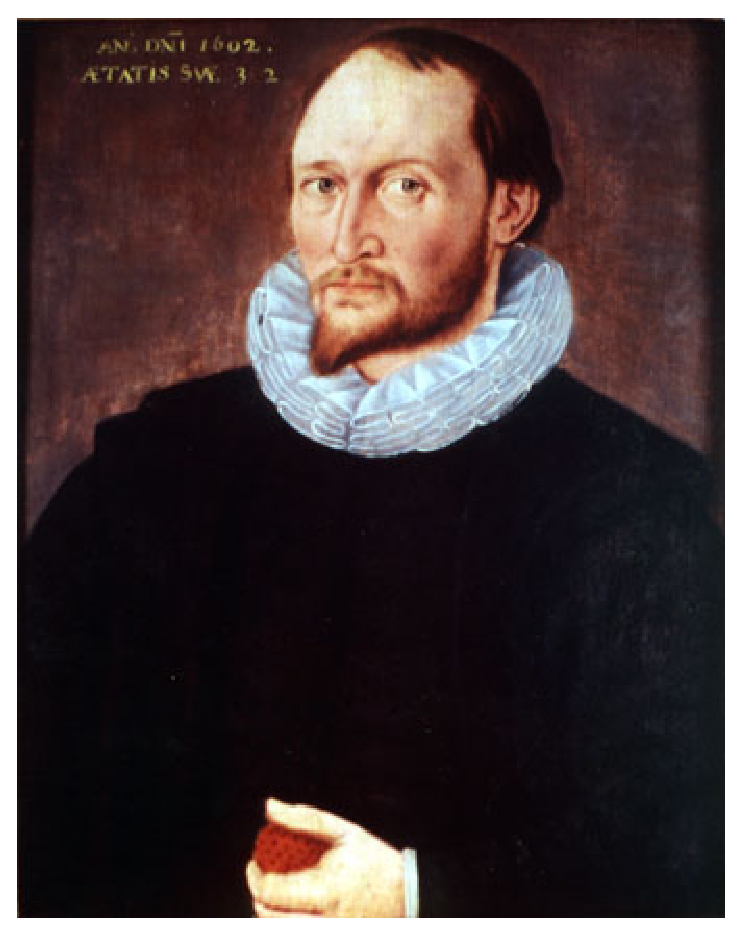
\includegraphics[scale=0.25]{harriot.eps}\\
\emph{{\small Thomas Harriot}}\\
\href{http://www.luminarium.org/renlit/hariot.htm}{www.luminarium.org/renlit/hariot.htm}\\[5mm]
\end{center}



3009-- Laquelle des fractions suivantes est une fraction \og \emph{bien \'ecrite} \fg \ pour les \'Egyptiens?\\

a) $\frac{1}{100}$\\[2mm]
b) $\frac{2}{5}$\\[2mm]
c) $\frac{5}{6}$\\[2mm]
d) $\frac{9}{10}$\\[2mm]

R\'eponse : a)\\

R\'etroaction :\\
Une fraction \og \emph{bien \'ecrite} \fg \ (plus couramment appel\'ee une \og \emph{fraction \'egyptienne} \fg) est une fraction dont le num\'erateur est \'egal \`a 1. Donc la r\'eponse est a).\\



3010-- Qui ont \'et\'e les premiers \`a instaurer des syt\`emes de mesure en base 60 (par exemple, $360^{\circ}$ dans un cercle, $60$ secondes dans une minute, $60$ minutes dans une heure) ?\\

a) les Arabes\\
b) les Grecs\\
c) les hommes pr\'ehistoriques\\
d) le groupe des 60\\

R\'eponse : b)\\

R\'etroaction :\\
Les Arabes travaillaient avec la base 10 (les chiffres arabes sont les chiffres que nous utilisons encore aujourd'hui: \og$0, 1, 2, 3, 4, 5, 6, 7, 8, 9$\fg). Les Babyloniens travaillaient d\'ej\`a en base 60, mais ce sont les Grecs qui ont \'etabli les syst\`emes de mesure en base 60 que nous connaissons aujourd'hui (60 secondes dans une minute, 60 minutes dans une heure). Donc la r\'eponse est b).\\



3011-- Dans des manuscrits russes du {\scriptsize XVII\ieme{}} si\`ecle, on retrouve le dessin suivant:\\
\begin{center}
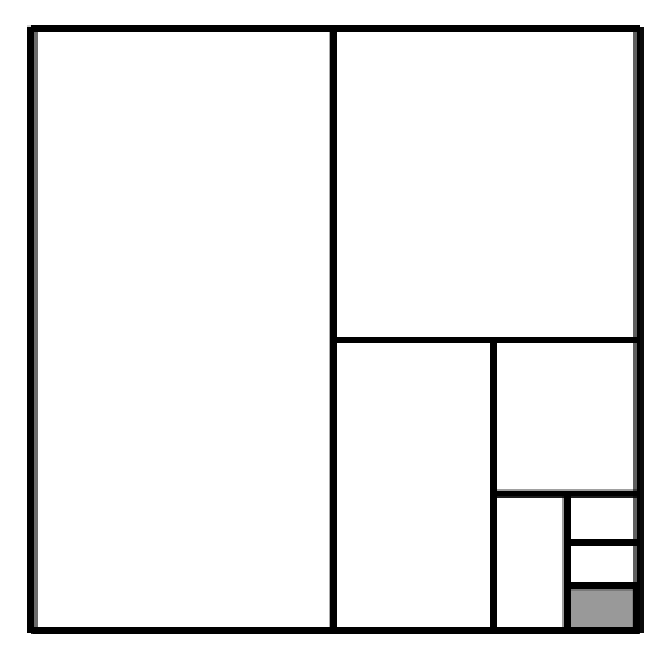
\includegraphics[scale=0.3]{carre_proportions.eps}
\end{center}
Quelle fraction  correspond \`a la partie ombr\'ee?\\

a) $\frac{1}{96}$\\[2mm]
b) $\frac{1}{64}$\\[2mm]
c) $\frac{1}{16}$\\[2mm]
d) $\frac{1}{8}$\\

R\'eponse : a)\\

R\'etroaction :\\
Dans les manuscrits russes, la partie ombr\'ee est d\'ecrite comme la \og \emph{moiti\'e de la moiti\'e de la moiti\'e de la moiti\'e de la moiti\'e du tiers} \fg. Autrement dit,
\begin{eqnarray*}
\frac{1}{2} \times \frac{1}{2} \times \frac{1}{2} \times \frac{1}{2} \times \frac{1}{2} \times \frac{1}{3} = \frac{1}{96}
\end{eqnarray*}
Donc la r\'eponse est a).\\



3012-- Qui utilisaient les fractions comme nous le faisons de nos jours?\\

a) les Babyloniens\\
b) les Chinois\\
c) les Hommes de Cro-Magnon\\
d) les Martiens\\

R\'eponse : b)\\

R\'etroaction :\\
100 avant J\'esus-Christ, les Chinois utilisaient les fractions comme nous le faisons, \`a une chose pr\`es: ils \'evitaient les fractions \og \emph{impropres} \fg, c'est-\`a-dire les fractions de la forme $\frac{7}{3}$. Ils \'ecrivaient plut\^ot $2 \frac{1}{3}$. La r\'eponse est b).\\



3013-- Les Chinois utilisaient la m\'ethode du d\'enominateur commun pour diviser deux fractions, par exemple, $\frac{2}{3} \div \frac{4}{5}$. La m\'ethode dit que l'on doit d'abord multiplier les num\'erateurs et les d\'enominateurs de chaque fraction par le d\'enominateur de l'autre fraction:\\
\begin{eqnarray*}
\frac{2}{3} \ \div \ \frac{4}{5} \ = \ \frac{2\cdot5}{3\cdot5} \ \div \ \frac{3\cdot4}{3\cdot5} \ = \ \frac{10}{15} \ \div \ \frac{12}{15}.
\end{eqnarray*}
Comme les deux fractions sont maintenant sur le m\^eme d\'enominateur, le probl\`eme se r\'eduit \`a une division de nombres entiers:
\begin{eqnarray*}
\frac{2}{3} \ \div \ \frac{4}{5} \ = \ \frac{10}{15} \ \div \ \frac{12}{15} \ = \ 10 \ \div \ 12 \ = \ \frac{5}{6}.
\end{eqnarray*}
En utilisant cette m\'ethode, calcule $\frac{3}{4} \ \div \ \frac{9}{11}$.\\

R\'eponse : $\frac{11}{12}$\\

R\'etroaction :\\
\begin{eqnarray*}
\frac{3}{4} \ \div \ \frac{9}{11} \ &=& \ \frac{3\cdot11}{4\cdot11} \ \div \ \frac{4\cdot9}{4\cdot11}\\[2mm]
&=& \ \frac{33}{44} \ \div \ \frac{36}{44}\\[2mm]
&=& \ 33 \ \div \ 36\\[2mm]
&=& \ \frac{11}{12}
\end{eqnarray*}
Donc la r\'eponse est $\frac{11}{12}$.\\



3014-- La m\'ethode de multiplication par l'inverse consiste \`a inverser le diviseur et de le multiplier au dividende. Par exemple,
\begin{eqnarray*}
\frac{2}{3} \ \div \ \frac{4}{5} \ = \ \frac{2}{3} \ \times \ \frac{5}{4} \ = \ \frac{10}{12} \ = \ \frac{5}{6}.
\end{eqnarray*}
Aux environs de 850 apr\`es J\'esus-Christ, qui a \'et\'e le premier \`a utiliser cette m\'ethode?\\

a) Apollonius\\
b) Ren\'e Descartes\\
c) Mahavira\\
d) Multit Plie Kassion\\

R\'eponse : c)\\

R\'etroaction :\\
La m\'ethode de multiplication par l'inverse n'a du sens que si la fraction est \'ecrite un nombre par dessus l'autre. Or, ce sont les Indiens qui, les premiers, \'ecrivaient les fractions de cette mani\`ere. Alors, c'est le math\'ematicien indien Mahavira qui utilisait la m\'ethode de multiplication par l'inverse vers 850 apr\`es J\'esus-Christ. Donc, la r\'eponse est c).\\



3015-- Le terme \og \emph{pour cent} \fg \ (pourcentage) est le nom donn\'e aux fractions dont le d\'enominateur est 100. C'est aux {\scriptsize XV\ieme{}} et {\scriptsize XVI\ieme{}} si\`ecles qu'on utilise pour la premi\`ere fois ce terme dans un contexte autre que les math\'ematiques pures. Lequel?\\

a) Commerce\\
b) Imp\^ots\\
c) M\'edecine\\
d) Urbanisation\\

R\'eponse : a)\\

R\'etroaction :\\
Il \'etait commun \`a l'\'epoque de calculer les taux d'int\'er\^ets commerciaux en utilisant le pourcentage. La r\'eponse est donc a). Une telle habitude est rest\'ee jusqu'\`a aujourd'hui, en affaires. C'est \'egalement une des raisons pour laquelle notre syst\`eme mon\'etaire est bas\'e sur le dollar et le \og \emph{cent} \fg.\\



3016-- Lequel de ces symboles n'a jamais \'et\'e utilis\'e pour repr\'esenter un pourcentage?\\

a) pour 100\\[2mm]
b) $\frac{0}{0}$\\[2mm]
c) \%\\[2mm]
d) $\scriptstyle0/100$\\[2mm]

R\'eponse : d)\\

R\'etroaction :\\
\begin{center}
\begin{tabular}{|c|c|}
\multicolumn{2}{c}{\bf \'Evolution du symbole de pourcentage}\\[2mm] \hline
{\bf Ann\'ee} & {\bf Symbole} \\[1mm] \hline \hline
1425 & \og \emph{pour cent} \fg \ \`a la main \\[1mm] \hline
vers 1650 & \og pour $\frac{0}{0}$ \fg \\[1mm] \hline
quelques ann\'ees plus tard & \og $\frac{0}{0}$ \fg \\[1mm] \hline
aujourd'hui & \og \% \fg \\[1mm] \hline
\multicolumn{2}{c}{}
\end{tabular}
\end{center}
Le symbole qui n'a jamais exist\'e est \og $\scriptstyle0/100$ \fg. La r\'eponse est d).\\



3017-- \`A quel si\`ecle l'\'ecriture des chiffres en notation d\'ecimale (par exemple 0,25) a-t-elle \'et\'e popularis\'ee?\\

a) {\scriptsize III\ieme{}} si\`ecle\\
b) {\scriptsize XVI\ieme{}} si\`ecle\\
c) {\scriptsize XVII\ieme{}} si\`ecle\\
d) {\scriptsize XXI\ieme{}} si\`ecle\\

R\'eponse : b)\\

R\'etroaction :\\
C'est en 1585, dans un livre du math\'ematicien belge, Simon Stevin, que l'\'ecriture des fractions en nombres d\'ecimaux est montr\'ee comme \'etant plus simple. La r\'eponse est donc b). Pour Stevin, le nombre d\'ecimal $0,333$ est une bonne approximation de la fraction $\frac{1}{3}$. On sait aujoud'hui que $\frac{1}{3} = 0,\overline3$, c'est-\`a-dire qu'il existe une quantit\'e infinie de 3 apr\`es la virgule.\\
\begin{center}
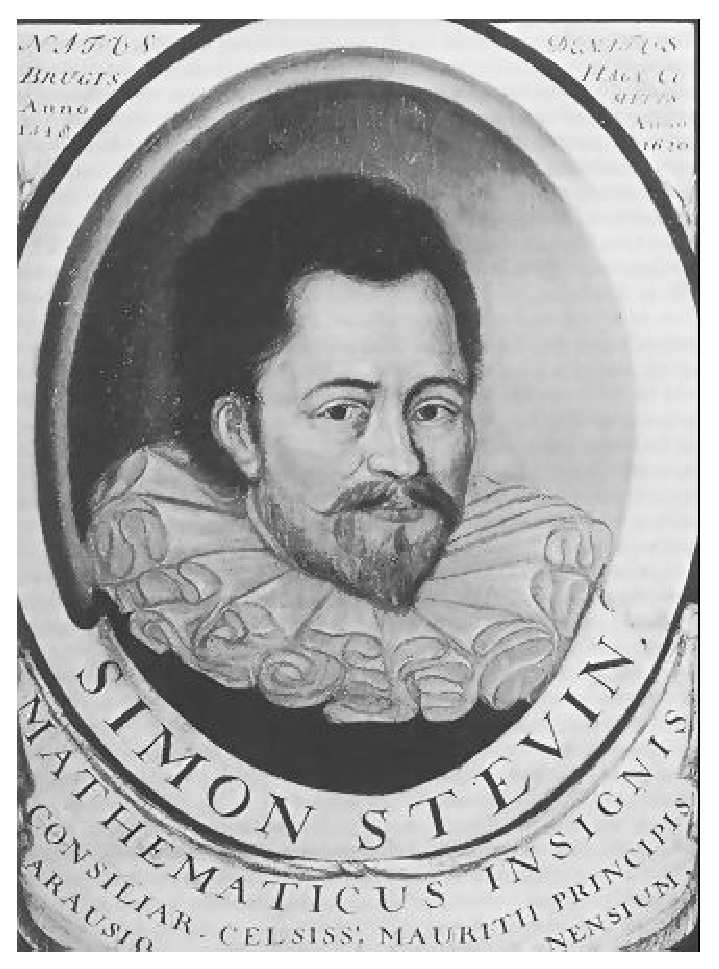
\includegraphics[scale=0.25]{stevin.eps}\\
\emph{{\small Simon Stevin}}\\
\href{http://fr.wikipedia.org/wiki/Simon Stevin}{fr.wikipedia.org/wiki/Simon Stevin}[5mm]
\end{center}



3018-- En quelle ann\'ee le premier livre d'arithm\'etique utilisant la virgule pour s\'eparer la partie enti\`ere de la partie fractionnaire a-il \'et\'e imprim\'e en Am\'erique?\\

a) 500 avant J\'esus-Christ\\
b) 1300\\
c) 1729\\
d) 1919\\

R\'eponse : c)\\

R\'etroaction :\\
C'est en 1729 qu'un premier livre d'arithm\'etique, utilisant la virgule pour s\'eparer la partie enti\`ere de la partie fractionnaire, est imprim\'e en Am\'erique. Donc, la r\'eponse est c). Par la suite, certains livres utilisaient le point. Aujourd'hui, on utilise la virgule en fran\c cais et le point en anglais.\\



3019-- Quel math\'ematicien flamand (un belge) est le premier \`a voir les nombres r\'eels ($\mathbb{R}$) comme les points d'une droite?\\

a) Gerardus Mercator\\
b) Nicolas Copernic\\
c) Gesuit Bellje\\
d) Simon Stevin\\

R\'eponse : d)\\

%{\bf\textsf{animation : chaque description du math\'ematicien appara\^it avec son image : le petit bonhomme pourrait les pousser ou tirer, sur son skateboard}}\\
R\'etroaction :\\
Gerardus Mercador est un math\'ematicien g\'eographe qui a fait la premi\`ere projection de la terre (c'est-\`a-dire, la premi\`ere carte).
\begin{center}
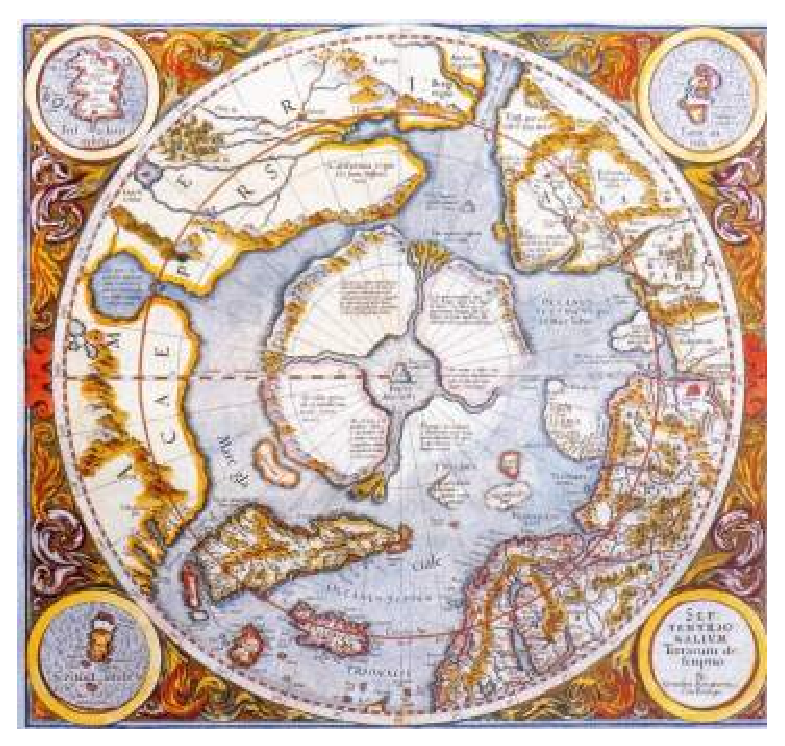
\includegraphics[scale=0.3]{carte.eps}\\
\emph{{\small carte du P\^ole Nord par Gerardus Mercator (fin du 16\ieme{} si\`ecle)}}\\
\href{http://www.transpolair.com/images/cart161.jpg}{www.transpolair.com/images/cart161.jpg}
\end{center}
Nicolas Copernic, m\'edecin et astronome polonais, dessine le premier mod\`ele h\'eliocentrique du syst\`eme solaire (h\'eliocentrique veut dire dont le soleil est au centre). Il a donc imagin\'e le syst\`eme solaire comme on le conna\^it aujourd'hui.
\begin{center}
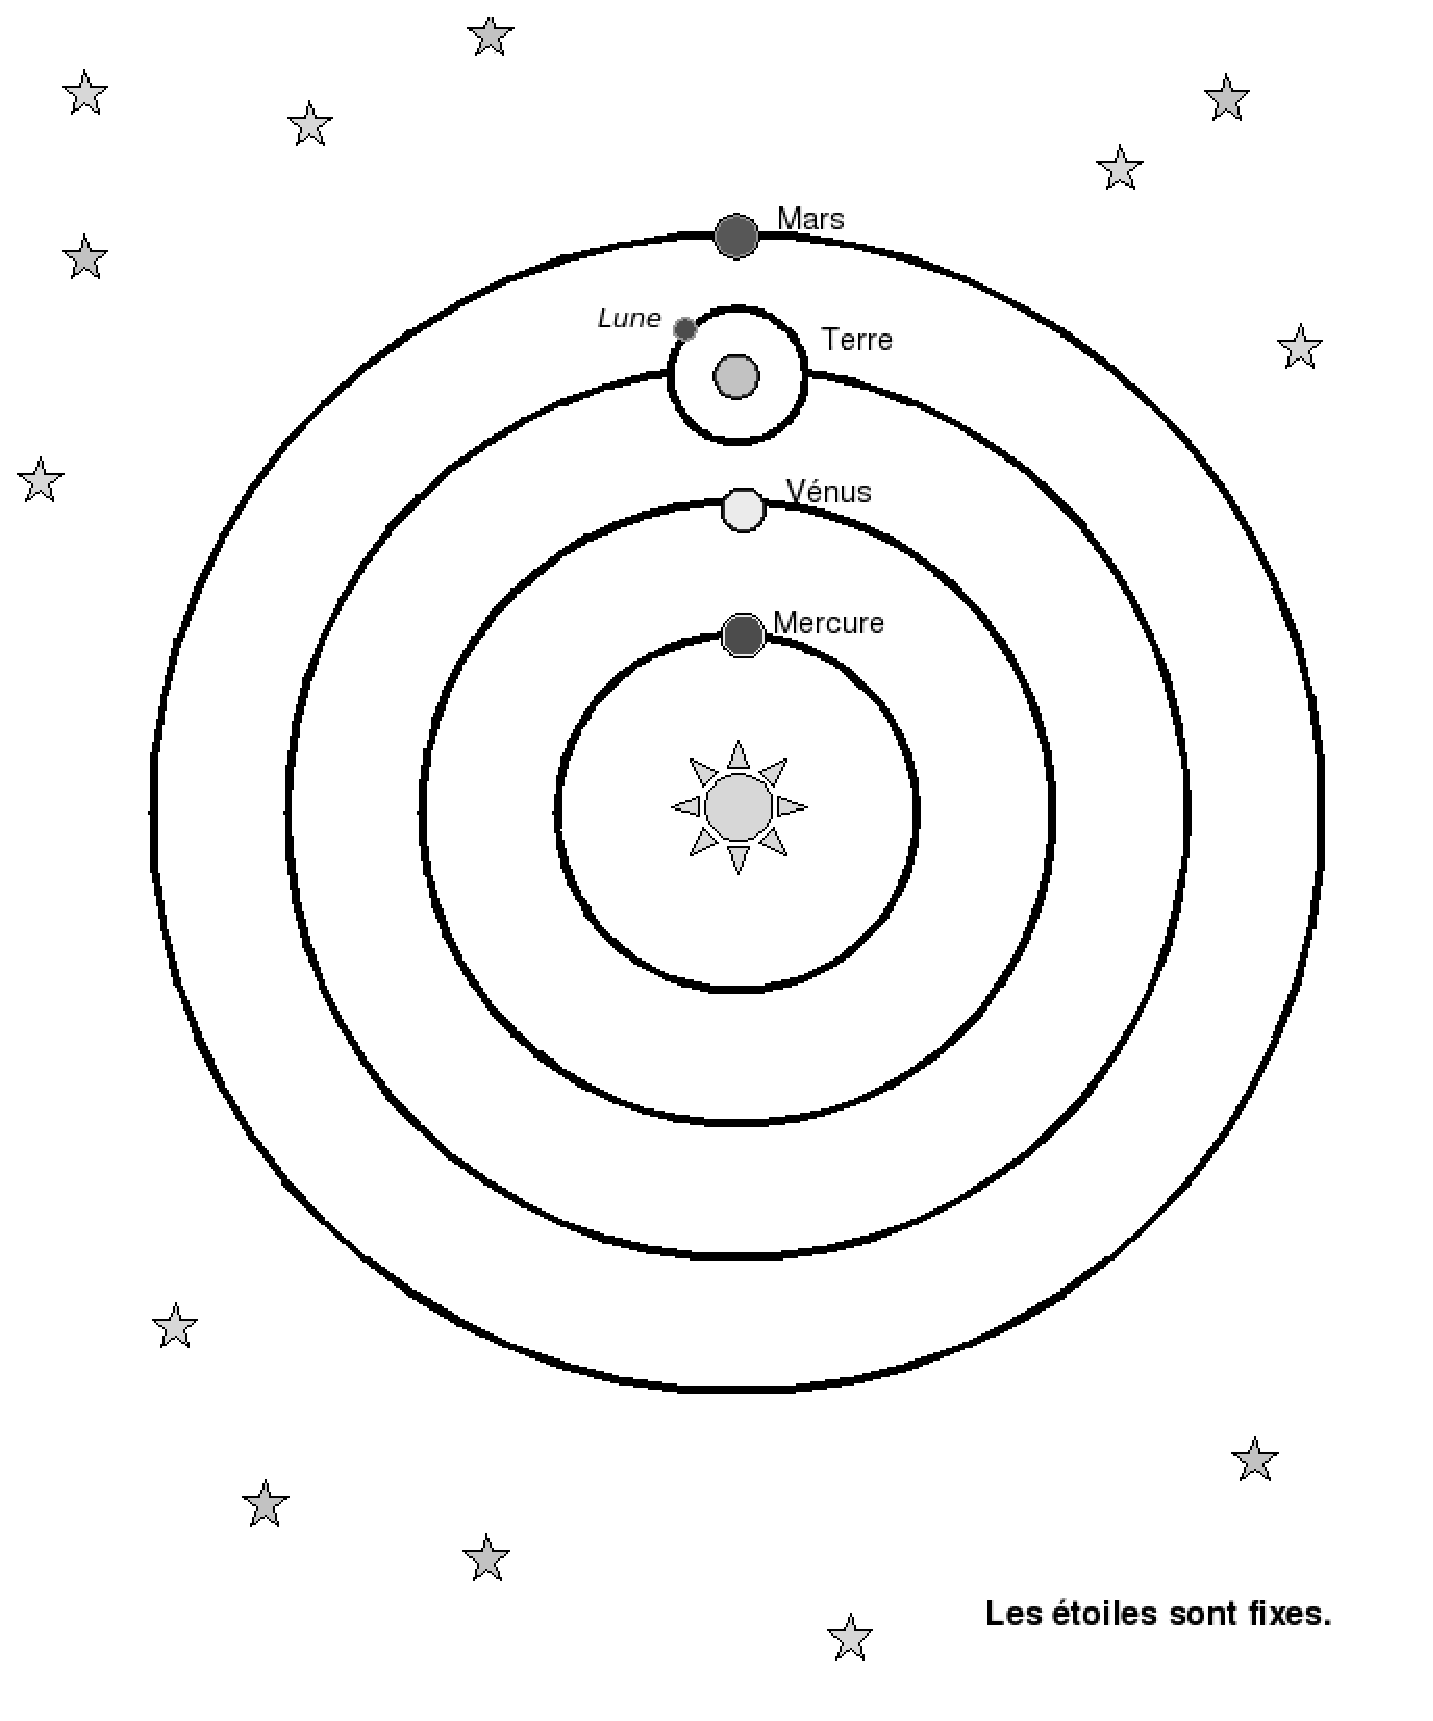
\includegraphics[scale=0.25]{heliocentrique.eps}\\
\emph{{\small syst\`eme copernicien, h\'eliocentrique}}
\end{center}

Et finalement, Simon Stevin a \'et\'e le premier math\'ematicien \`a voir les nombres r\'eels comme les points d'une droite. La r\'eponse est d).\\
\begin{center}
\includegraphics[scale=0.25]{droitereelle.eps} {\large$\mathbb{R}$}\\
\emph{{\small droite r\'eelle}}
\end{center}



3020-- D\`es 1500 avant J\'esus-Christ, les nombres n\'egatifs existaient.\\
Vrai ou Faux?\\

R\'eponse : Faux\\

R\'etroaction :\\
La r\'eponse est : faux. Lorsque Christophe Colomb a d\'ecouvert l'Am\'erique, les nombres n\'egatifs n'existaient pas. Ce n'est que 200 ans plus tard qu'on les a accept\'es dans la famille des nombres!\\
Les nombres servaient au d\'epart \`a compter des objets. Lorsque les gens de l'\'epoque ont accept\'e le chiffre 0, c'\'etait le plus petit nombre. Qu'est-ce qui peut \^etre plus petit que rien du tout?\\ (Les math\'ematiciens savaient qu'il existait de tels nombres, mais dans leurs probl\`emes, comme par exemple trouver la solution de $4x + 20 = 4$, il rejetait tout simplement les solutions n\'egatives (cette \'equation n'avait pas de solution \`a l'\'epoque, bien que $x = -4$ soit une solution!)).\\



3021-- Quel est le premier math\'ematicien indien \`a avoir travaill\'e avec des \og quantit\'es \fg \ n\'egatives? (on ne parle pas de nombres ici, mais bien de quantit\'es)\\

a) Brahmagupta\\
b) Havoire D\'ed\`ete\\
c) Carl Friedrich Gauss\\
d) Pythagore\\

R\'eopnse : a)\\

R\'etroaction :\\
Un math\'ematicien indien, Brahmagupta {\small(598-668)}, tra\^itait des avoirs (quantit\'es positives) et des dettes (quantit\'es n\'egatives). Il a m\^eme \'etabli des r\`egles pour additionner, soustraire, multiplier et diviser les avoirs et les dettes. La r\'eponse est donc a).\\



%{\bf\textsf{animation : petit bonhomme avec tout plein de points d'interrogation autour de sa t\^ete}}\\
3022-- \og \emph{Si $-1$ est plus petit mais pas \'egal \`a 1, alors $\frac{-1}{1} = \frac{1}{-1}$ n'a aucun sens, car le plus petit nombre sur le plus grand ne peut pas \^etre \'egal au plus grand sur le plus petit} \fg. \ Par exemple : $1 < 3 \ \textrm{et} \ \frac{1}{3} \neq \frac{3}{1}$.\\[2mm]
Quel math\'ematicien du {\scriptsize XVII\ieme{}} si\`ecle a soulev\'e cette question?\\

a) Antoine Arnauld\\
b) Euclide\\
c) Omar Khayyam\\
d) Sim\'eon-Denis Poisson\\

R\'eponse : a)\\

R\'etroaction :\\
M\^eme apr\`es avoir accept\'e les nombres n\'egatifs dans la famille des nombres, les math\'ematiciens du {\scriptsize XVII\ieme{}} si\`ecle \'eprouvaient de la difficult\'e \`a les ordonner. Comment $-1$ peut-il \^etre plus petit que 1, alors que leur ratio, $\frac{-1}{1}$ et $\frac{1}{-1}$ sont \'egaux? Celui qui a soulev\'e cette question est Antoine Arnauld {\small (1612-1694)}. La r\'eponse est donc a).

\begin{center}
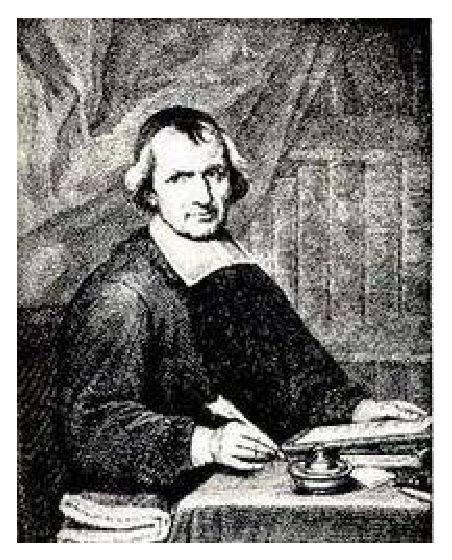
\includegraphics[scale=0.5]{Antoine_Arnauld.eps}\\
\emph{{\small Antoine Arnauld}}\\
\href{http://fr.wikipedia.org/wiki/Antoine Arnauld}{fr.wikipedia.org/wiki/Antoine Arnauld}\\[5mm]
\end{center}



3023-- Quel math\'ematicien croyait (m\^eme si on sait de nos jours que ce n'est pas vrai) et a montr\'e que les nombres n\'egatifs \'etaient plus grands que l'infini ($\infty$)?\\

a) Georges Cantor\\
b) Henri Navier\\
c) John Wallis\\
d) Joseph Fourier\\

R\'eponse : c)\\

R\'etroaction :\\
C'est dans le livre \og \emph{Arithmetica Infinitorum} \fg \ de John Wallis que l'on retrouve l'\'enonc\'e \og \emph{les nombres inf\'erieurs \`a 0 sont plus grands que l'infini} \fg. \ La r\'eponse est c), John Wallis.
\begin{center}
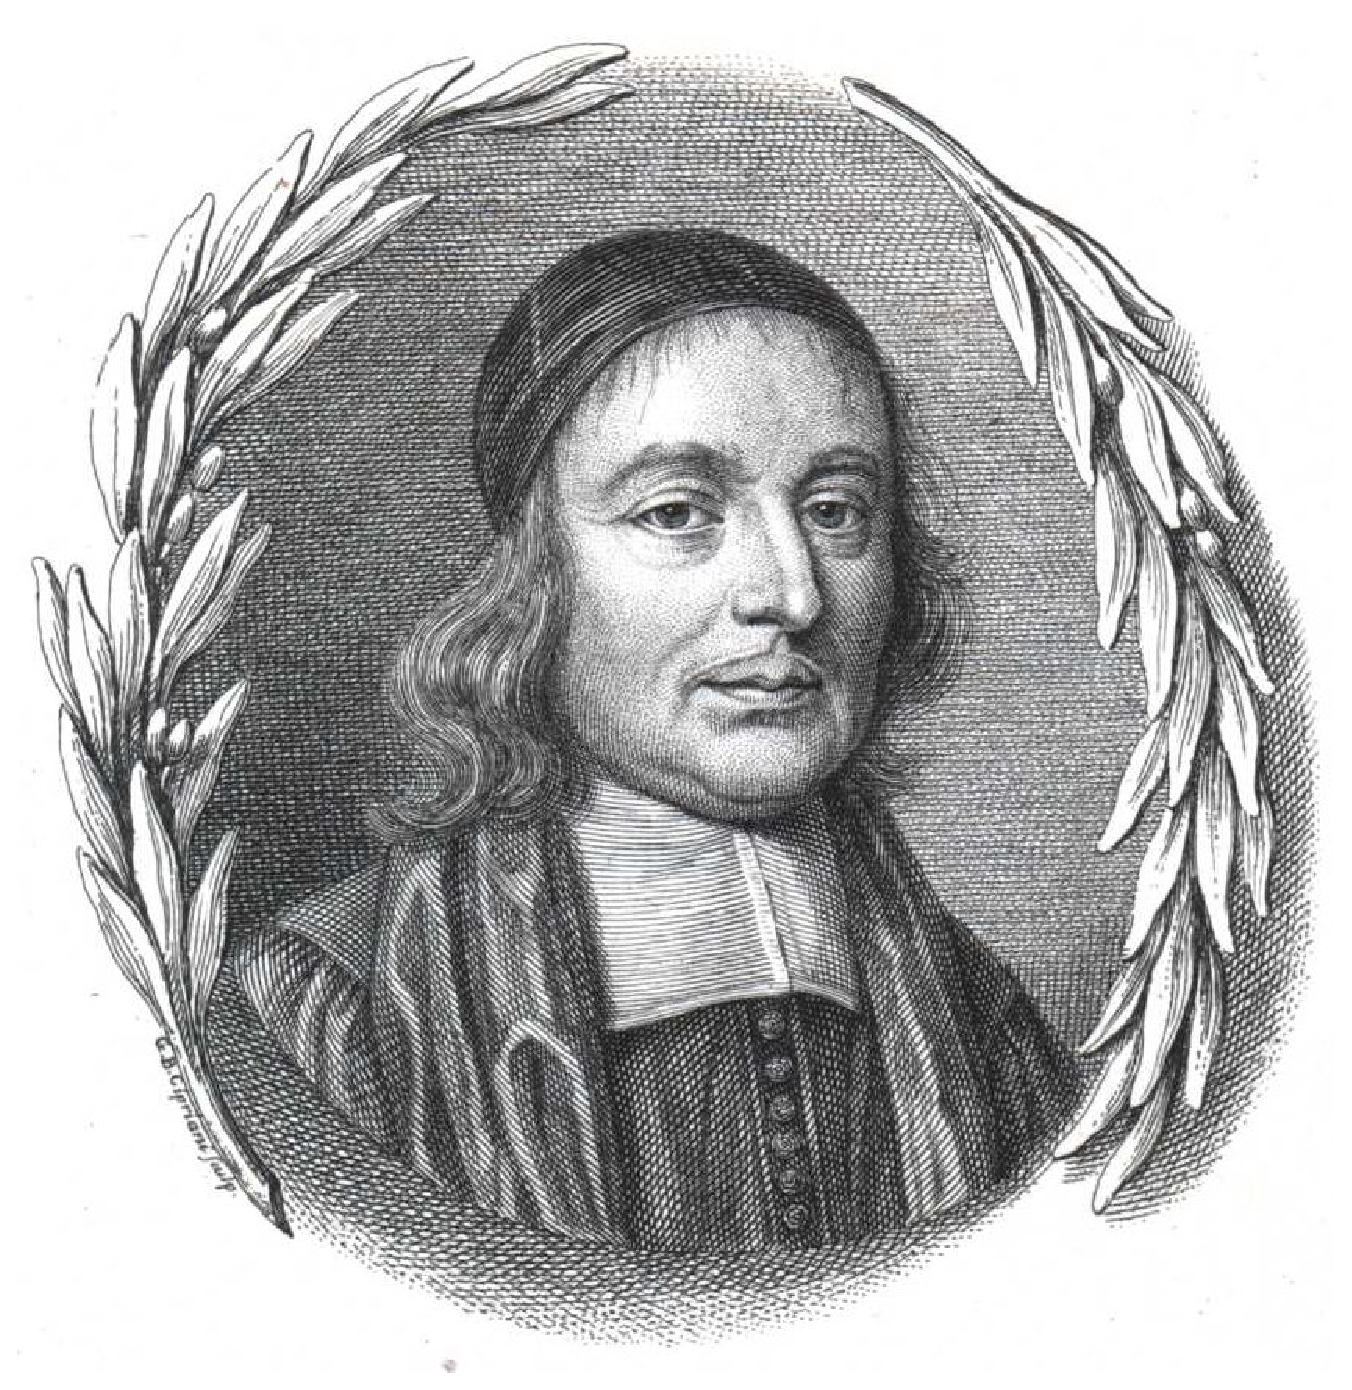
\includegraphics[scale=0.2]{John_Wallis.eps}\\
\emph{{\small John Wallis}}\\
\href{http://fr.wikipedia.org/wiki/John Wallis}{fr.wikipedia.org/wiki/John Wallis}
\end{center}

Explication du raisonnement: \emph{Comme \ $\frac{3}{0} = \infty$, si on prend un d\'enominateur plus petit que $0$, alors la nouvelle fraction devrait \^etre plus grande que $\frac{3}{0}$ (par exemple, comme $1 < 2$, alors $3 = \frac{3}{1} > \frac{3}{2} = 1,5$). Ainsi, comme $-1 < 0$, alors $\frac{3}{-1} > \frac{3}{0} = \infty$. On sait maintenant que m\^eme si $-1 < 0$, on a que $-3 = \frac{3}{-1} < \frac{3}{0} = \infty$.}\\



3024-- Quel physicien anglais bien connu, qui \'etait \'egalement math\'ematicien, a dit la phrase suivante : \og \emph{Les quantit\'es sont positives et plus grandes que rien ou n\'egatives et plus petites que rien.}\fg?\\

a) Georges Adams\\
b) Isaac Newton\\
c) Johnny Test\\
d) Michel Rolle\\

R\'eponse : b)\\

R\'etroaction :\\
Contrairement \`a ce que l'on pourrait croire, Isaac Newton n'a pas seulement travaill\'e en physique. C'est en 1707, dans son livre \og \emph{Universal Arithmetick} \fg, qu'il a \'ecrit que les quantit\'es positives sont plus grandes que rien et les n\'egatives, plus petites que rien. Comme Newton \'etait un scientifique important de l'\'epoque, son id\'ee a \'et\'e prise tr\`es au s\'erieux. Donc, la r\'eponse est b).\\

\begin{center}
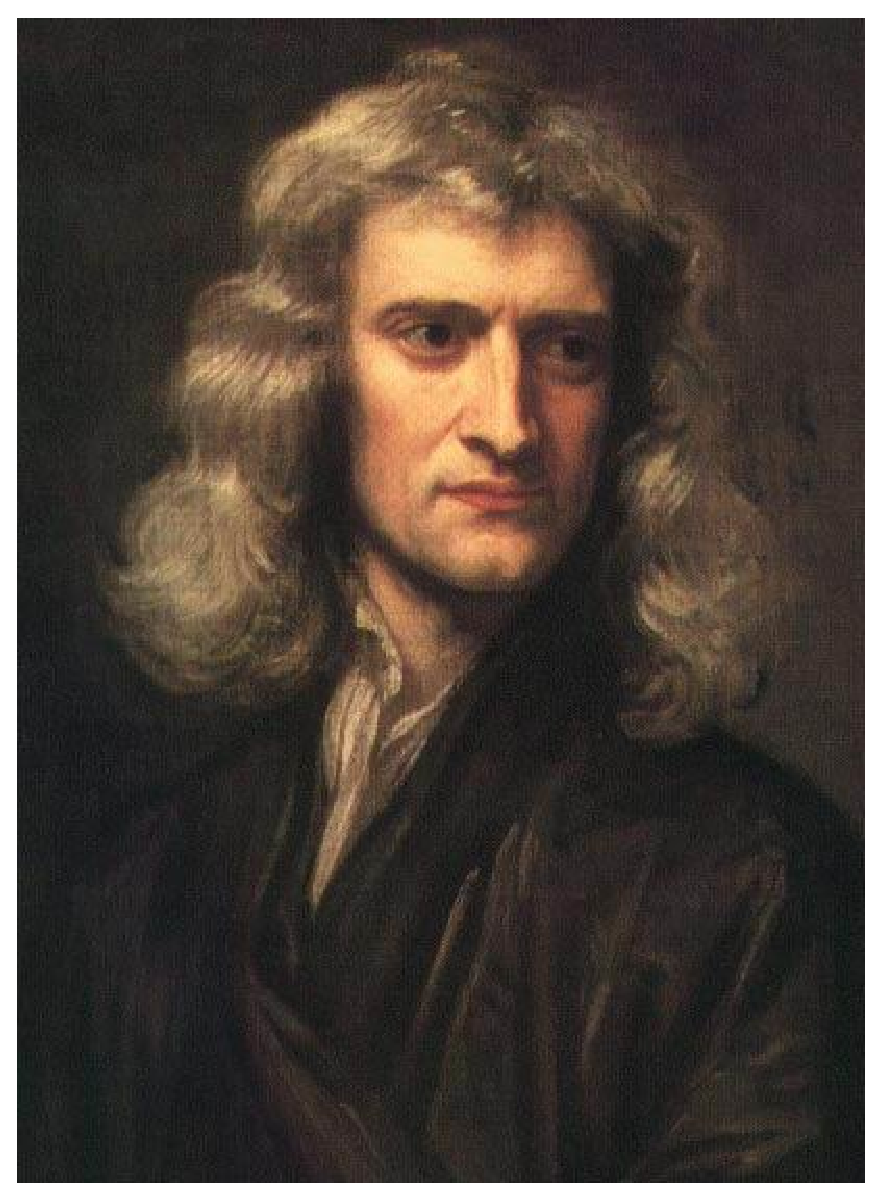
\includegraphics[scale=0.2]{IsaacNewton.eps}\\
\emph{{\small Isaac Newton}}\\
\href{http://fr.wikipedia.org/wiki/Isaac Newton}{fr.wikipedia.org/wiki/Isaac Newton}\\[5mm]
\end{center}



3025-- Quel math\'ematicien suisse du {\scriptsize XVIII\ieme{}} si\`ecle a dit : \og \emph{Les nombres n\'egatifs peuvent \^etre consid\'er\'es comme des dettes, puisque les nombres positifs repr\'esentent des possessions r\'eelles. On peut dire que les nombres n\'egatifs sont moins que rien. Ainsi, quand un homme ne poss\`ede rien et qu'il doit 50 couronnes, il est certain qu'il a 50 couronnes de moins que rien. Si quelqu'un lui fait un cadeau de 50 couronnes pour payer ses dettes, il sera encore seulement \`a rien, mais il sera plus riche qu'avant}\fg ?\\[2mm]

a) Fran\c cois Vi\`ete\\
b) Jean-Marie De Koninck\\
c) Leonhard Euler\\
d) Pierre Fatou\\

R\'eponse : c)\\

R\'etroaction :\\
En 1770, dans \og \emph{Elements of Algebra} \fg, Leonhard Euler a repris, en quelque sorte, le raisonnement que les Chinois avaient fait 17 si\`ecles plus t\^ot, c'est-\`a-dire de voir les nombres positifs comme des avoirs et les n\'egatifs comme des dettes. La r\'eponse est c).\\

\begin{center}
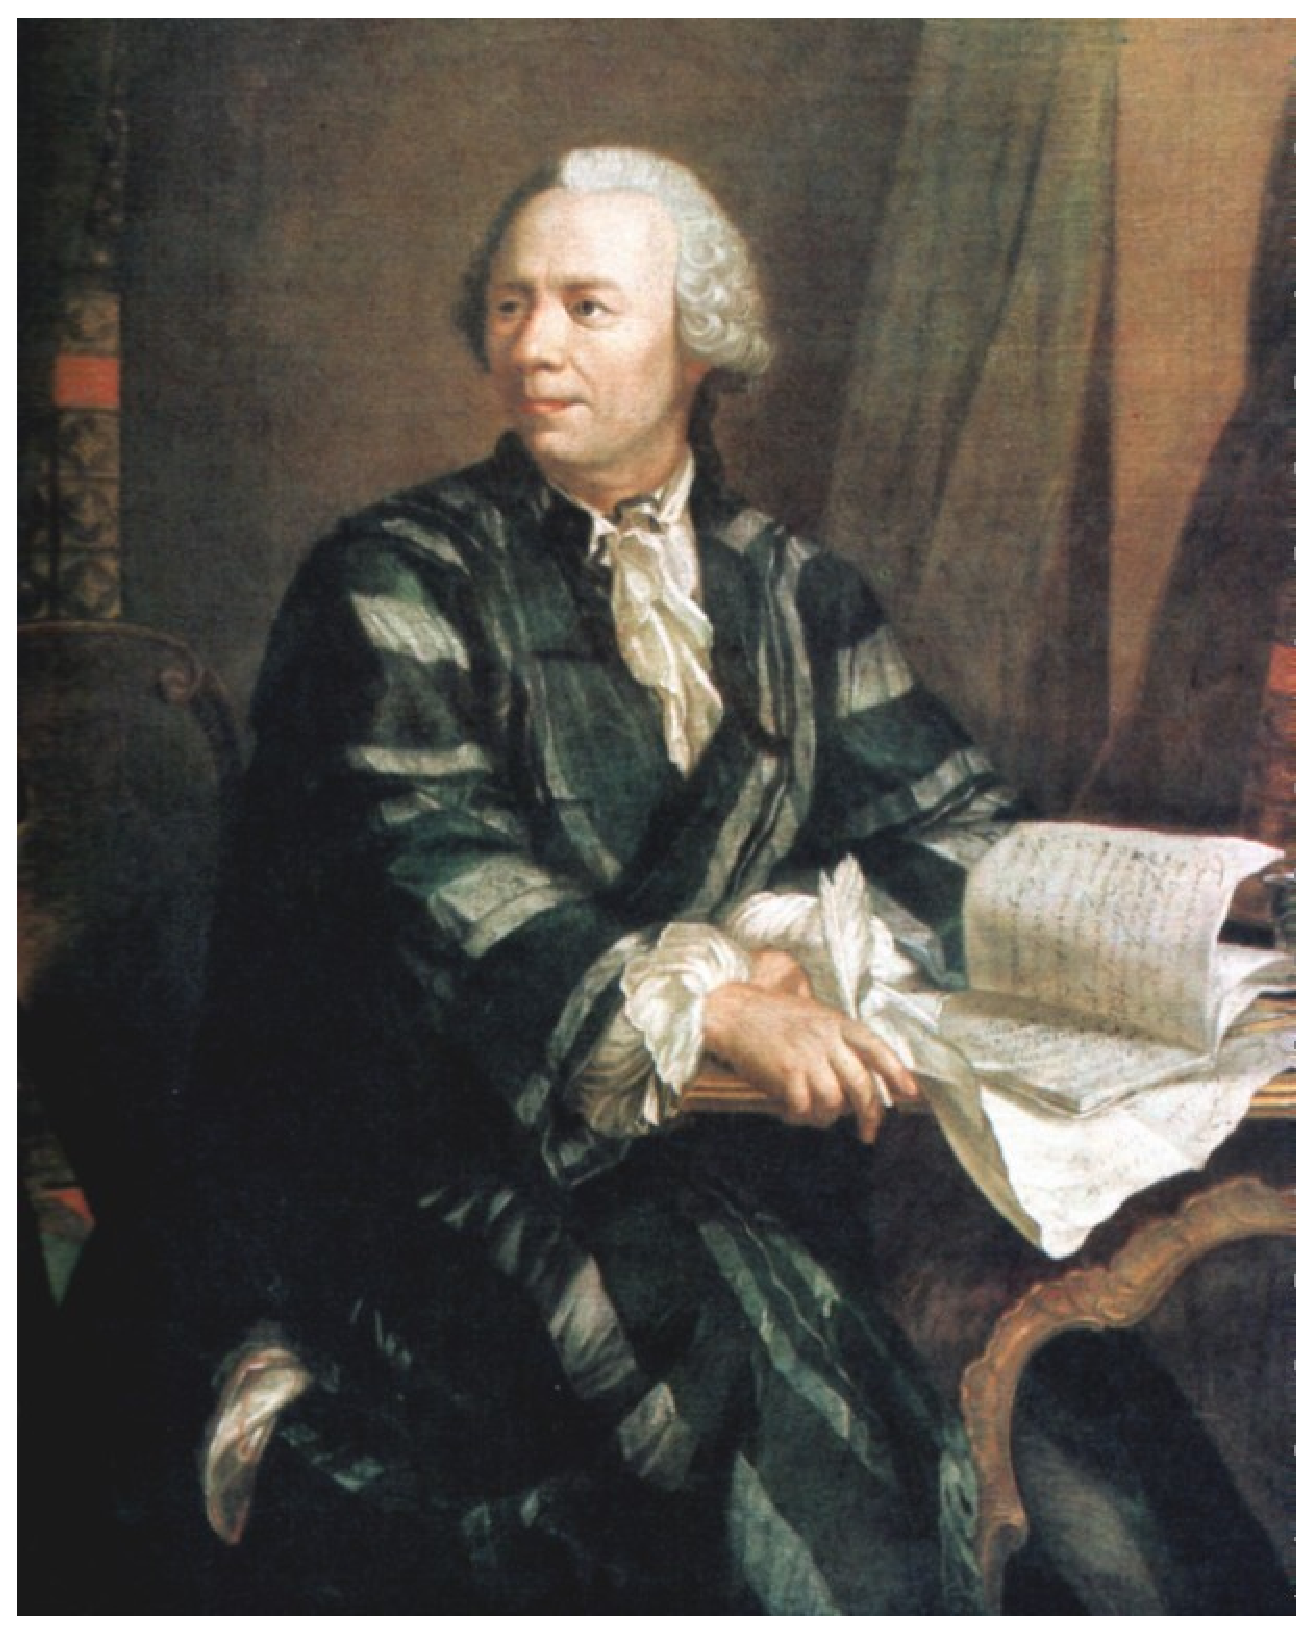
\includegraphics[scale=0.15]{Euler.eps}\\
\emph{{\small Leonhard Euler}}\\
\href{http://fr.wikipedia.org/wiki/Leonhard Euler}{fr.wikipedia.org/wiki/Leonhard Euler}\\[5mm]
\end{center}



3026-- \'Evariste Galois est un math\'ematicien fran\c cais n\'e en 1811, \`a Paris. Il est consid\'er\'e comme l'inventeur de la th\'eorie des groupes. En quelle ann\'ee est-il mort? (dites-vous que si on pose la question, c'est s\^urement pour une raison\dots)\\

\begin{center}
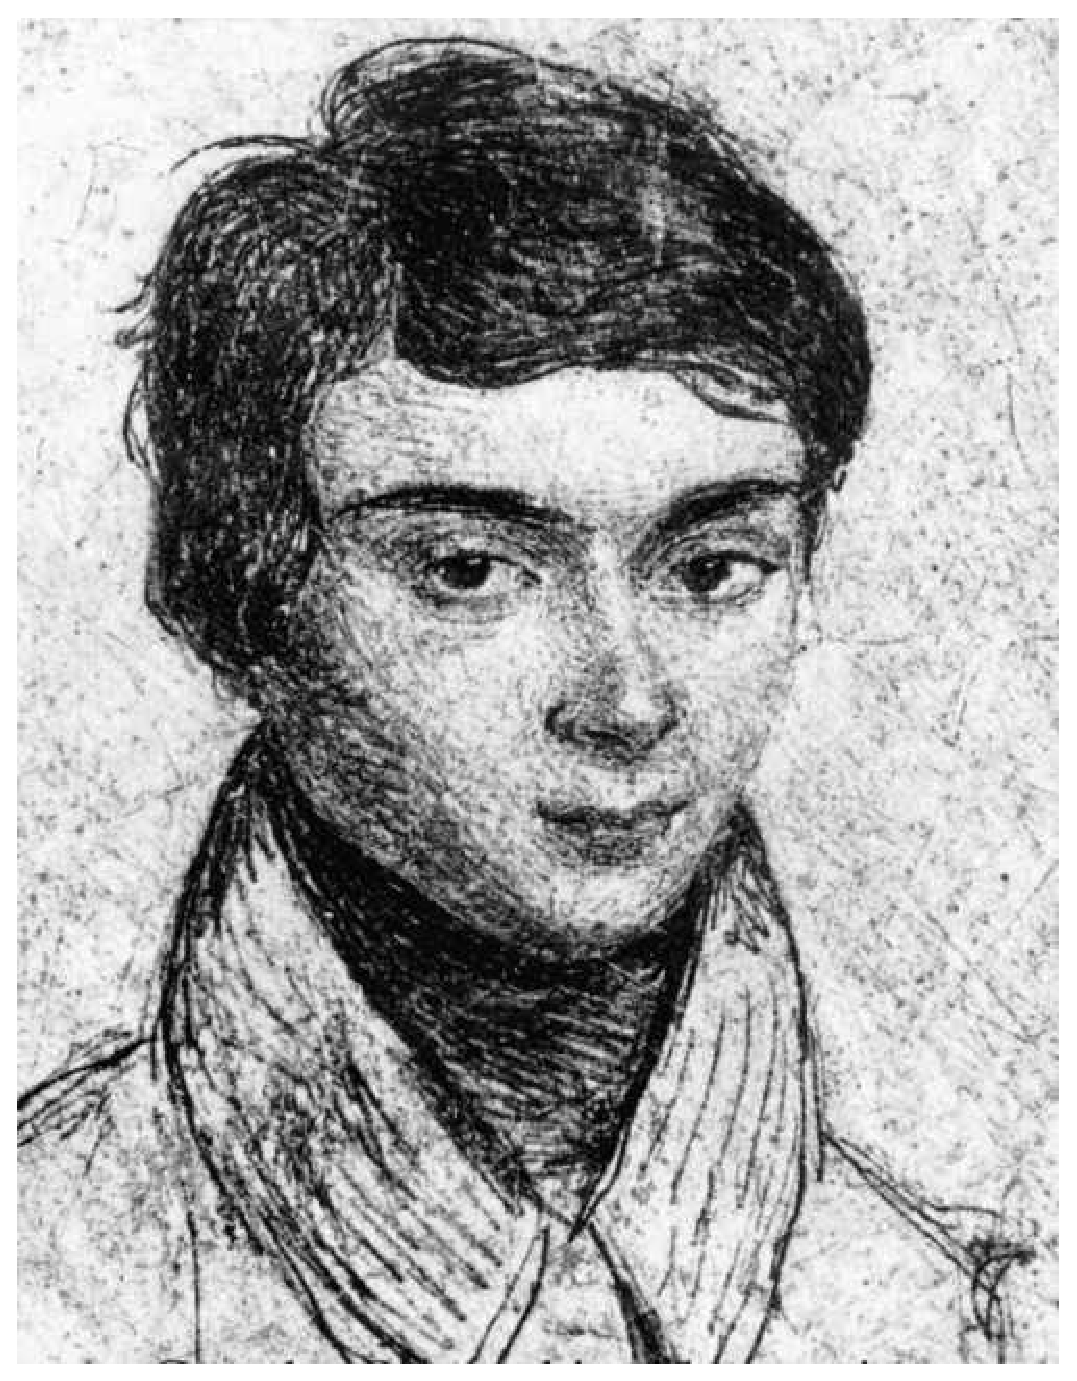
\includegraphics[scale=0.15]{Evariste_galois.eps}\\
\emph{{\small \'Evariste Galois}}\\
\href{http://fr.wikipedia.org/wiki/Evariste Galois}{fr.wikipedia.org/wiki/Evariste Galois}
\end{center}

a) 1832\\
b) 1855\\
c) 1870\\
d) 1911\\

R\'eponse : a)\\

%{\bf \textsf{animation : petit bonhomme pourrait faire de l'escrime}}\\
R\'etroaction :\\
Galois est d\'ec\'ed\'e en 1832, \`a l'\^age de 20 ans. Il est mort dans un duel pour d\'efendre l'honneur d'une femme. La r\'eponse est donc a).\\



3027-- Selon la l\'egende, sur quoi le roi Henry I\ier{} s'est-il bas\'e pour d\'ecider qu'une verge serait de 36 pouces?\\

a) Cette journ\'ee-l\`a, il avait chass\'e et avait attrap\'e un gibier qui mesurait 36 pouces.\\
b) Il avait de tr\`es grands pieds et la longueur totale de ses deux pieds ensemble \'etait de 36 pouces.\\
c) Lorsqu'il effectuait un grand pas devant lui, la distance entre le bout des orteils de son pied avant et le talon de son pied arri\`ere \'etait de 36 pouces.\\
d) Lorsqu'il \'etendait les bras droit devant lui, la distance entre le bout de son nez et ses pouces \'etait de 36 pouces.\\

R\'eponse : d)\\

%{\bf \textsf{animation : petit bonhomme, d\'eguis\'e en roi, qui mesure la distance de son nez \`a ses pouces}}\\
R\'etroaction :\\
Un jour, pour cesser toute confusion sur la mesure exacte d'une verge, le roi Henry I\ier{} d\'ecida quelle serait de longueur \'egale \`a la distance entre le bout de son nez et ses pouces. Il \'etira les bras devant lui et on mesura cette distance: \og \emph{36 pouces!} \fg. C'est alors qu'on d\'eclara officiellement qu'une verge vaut 36 pouces. La r\'eponse est d).\\



3028-- Le m\`etre a \'et\'e \'etabli comme le 10-millioni\`eme de la longueur de l'arc de la Terre au niveau de la mer, entre le P\^ole Nord et le P\^ole Sud.\\
Vrai ou Faux?\\

R\'eponse : Faux\\

R\'etroaction :\\
L'Acad\'emie des Sciences de France a d\'efini le m\`etre comme le 10-millioni\`eme de la longueur de l'arc de la Terre entre le P\^ole Nord et \emph{\underline{l'\'Equateur}}, et non le P\^ole Sud. La r\'eponse est: faux. La circonf\'erence de la Terre mesure environ $40\,000$ kilom\`etres. Le quart de la circonf\'erence, qui est en fait l'arc entre le P\^ole Nord et l'\'Equateur, mesure alors environ $10\,000$ kilom\`etres. Le 10-millioni\`eme de $10\,000$ kilom\`etres est 0,001 kilom\`etre, soit un m\`etre.
\begin{eqnarray*}
10\,000\,\text{km} \div 10\,000 000 &=& 0,001\,\text{km}\\
&=& 0,001\,\text{km} \times \frac{1\,000\,\text{m}}{1\,\text{km}}\\
&=& 1\,\text{m}\\
\end{eqnarray*}
\begin{center}
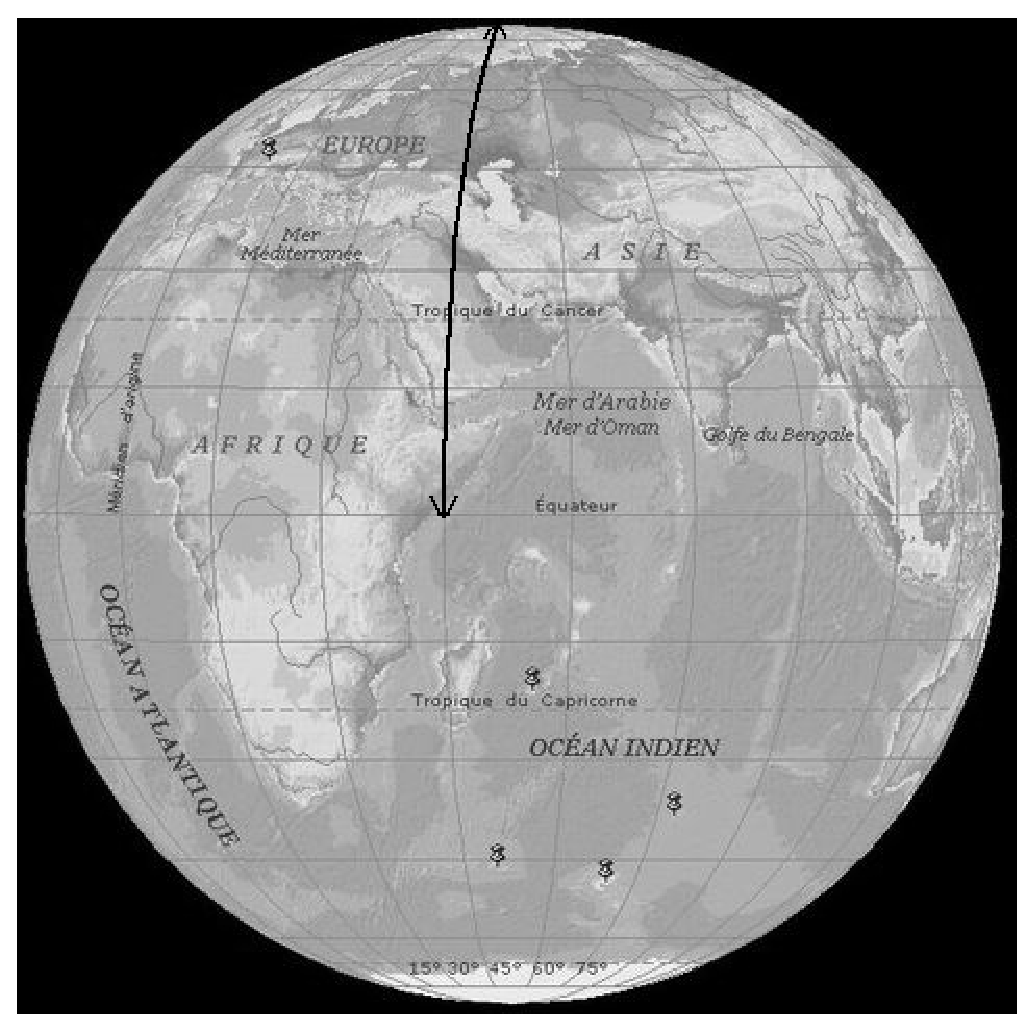
\includegraphics[scale=0.25]{terre.eps}\\
\href{http://collegevanoise.fr/images/ign/maurice.jpg}{collegevanoise.fr/images/ign/maurice.jpg}\\[5mm]
\end{center}



3029-- Les unit\'es plus petites que le m\`etre ont un pr\'efixe latin et les unit\'es plus grandes que le m\`etre ont un pr\'efixe grec.\\
Vrai ou Faux?\\

R\'eponse : Vrai\\

R\'etroaction :\\
Le fait que les unit\'es plus grandes ou plus petites que le m\`etre soient des puissances de 10 rend le syst\`eme m\'etrique plus facile \`a comprendre.\\

\begin{center}
\begin{tabular}{|l|c|l|} \hline
{\it Nom} & {\it Symbole} & {\it Nombre en chiffres}  \\ \hline \hline
\textbf{giga}m\`etre & Gm & $1 \, 000 \, 000 \, 000$\\ \hline
\textbf{m\'ega}m\`etre & Mm & $1 \, 000 \, 000$\\ \hline
\textbf{kilo}m\`etre & km & $1 \, 000$\\ \hline
\textbf{hecto}m\`etre & hm & $100$\\ \hline
\textbf{d\'eca}m\`etre & dam & $10$\\ \hline
m\`etre & m & $1$\\ \hline
\textbf{d\'eci}m\`etre & dm & $0,1$\\ \hline
\textbf{centi}m\`etre & cm & $0,01$\\ \hline
\textbf{milli}m\`etre & mm & $0,001$\\ \hline
\textbf{micro}m\`etre & $\mu$m & $0,000 \, 001$\\ \hline
\textbf{nano}m\`etre & nm & $0,000 \, 000 \, 001$\\ \hline
\multicolumn{3}{c}{}\\
\end{tabular}
\end{center}

Les pr\'efixes pour les unit\'es plus petites que le m\`etre (d\'eci-, centi-, milli-, \dots) sont latins. Les pr\'efixes pour les unit\'es plus grandes que le m\`etre (d\'eca-, hecto-, kilo-, \dots) sont grecs. La r\'eponse est : vrai.\\



3030-- Le kilogramme a \'et\'e d\'efini comme \'etant la masse de l'eau pure contenue dans un cube de un m\`etre de c\^ot\'e.\\
Vrai ou Faux?\\
\begin{center}
\includegraphics[scale=0.3]{cube.eps}
\end{center}

R\'eponse : Faux\\

%{\bf \textsf{animation : petit bonhomme pourrait intervenir ici $\rightarrow$ regarder ou lui-m\^eme remplir les cubes d'eau?}}\\
R\'etroaction :\\
Le kilogramme a \'et\'e d\'efini comme \'etant la masse de l'eau pure contenue dans un cube de un \emph{\underline{d\'ecim\`etre}} de c\^ot\'e et non de un m\`etre. La r\'eponse est : faux. Cette mesure est \'egale \`a un litre ($1\,\text{dm}^{3}\,=\,1\,\text{l}$).\\

\begin{center}
\includegraphics[scale=0.3]{cubedm.eps}
\end{center}



3031-- Quelle mesure d'angle a \'et\'e invent\'ee afin de pouvoir calculer la longueur de l'arc de la terre?\\

a) degr\'e\\
b) grade\\
c) radian\\
d) minute\\

R\'eponse : b)\\

R\'etroaction :\\
En voulant calculer la longueur de l'arc de la terre, des chercheurs engag\'es par l'Acad\'emie des Sciences de France ont d\'ecid\'e d'inventer une mesure d'angle qui utiliserait des puissances de 10, comme le syst\`eme m\'etrique. Ils pos\`erent donc la mesure de l'angle droit \'egale \`a 100 grades (90$^\circ$ = 100 gr). La r\'eponse est b).\\



3032-- \`A quel math\'ematicien allemand, n\'e en 1845,  doit-on la d\'efinition d'une fonction en terme d'ensemble de couples, c'est-\`a-dire de $y = f(x)$?\\

a) N\'een Dizuitcenkarantecink\\
b) Georg Cantor\\
c) Pythagore\\
d) William Brouncker\\

R\'eponse : b)\\

R\'etroaction :\\
Georg Cantor est l'initiateur de la th\'eorie des ensembles. Il a d\'efini une fonction comme un ensemble de couples. Une fonction peut alors \^etre dessin\'ee dans le plan cart\'esien, en fonction de $x$ et de $y$. Par exemple, $y = f(x) = x^{3} + x^{2} + x$.
%Cela a permis \`a Cantor de d\'efinir la fonction bijective ou bijection (si on prend un \'el\'ement $y$ dans l'ensemble d'arriv\'ee (image ou codomaine), alors il existe un et un seul \'el\'ement $x$ dans l'ensemble de d\'epart (domaine) qui est une solution de la fonction $y = f(x)$.
\begin{center}
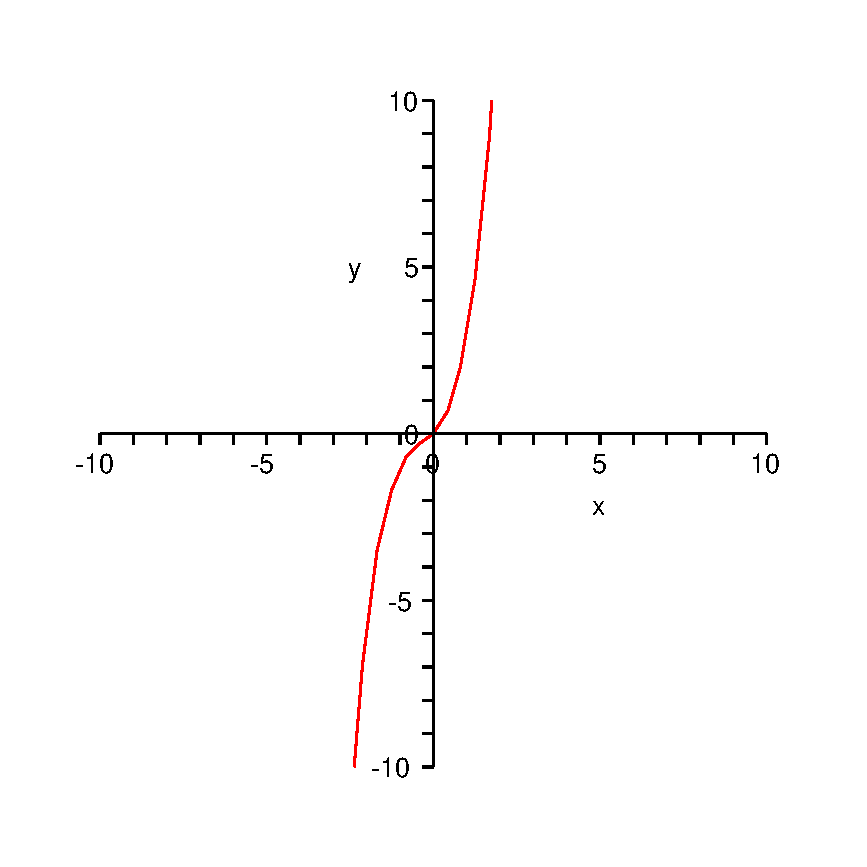
\includegraphics[scale=0.5]{fonction.eps}\\
$f(x) = x^{3} + x^{2} + x$\\
\end{center}
Donc, la r\'eponse est d).
\begin{center}
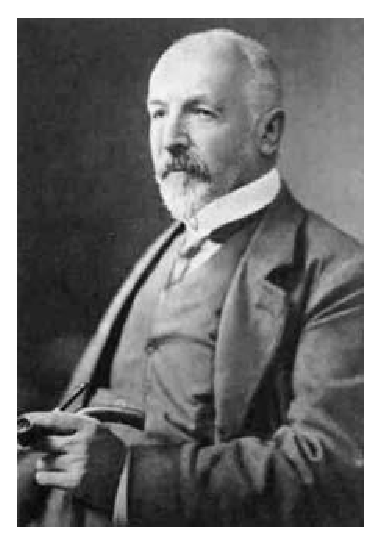
\includegraphics[scale=0.5]{Georg_Cantor.eps}\\
\emph{{\small Georg Cantor}}\\
\href{http://fr.wikipedia.org/wiki/Georg Cantor}{fr.wikipedia.org/wiki/Georg Cantor}\\[5mm]
\end{center}



%{\bf \textsf{animation : bonhomme d\'eguis\'e en Einstein qui regarde le mercure du thermom\`etre monter et descendre}}\\
3033-- En 1593, quel math\'ematicien a invent\'e le thermom\`etre?\\

a) Archim\`ede de Syracuse\\
b) Galileo Galilei\\
c) G\'erien Ninvent\'e\\
d) Leonard de Pise (dit Fibonacci)\\

R\'eponse : c)\\

R\'etroaction :\\
Archim\`ede de Syracuse a invent\'e, entre autres, une vis sans fin (la vis d'Archim\`ede). Galileo Galilei a construit le premier appareil permettant de comparer le niveau de chaud et de froid. La r\'eponse est donc c). L\'eonard de Pise a trouv\'e les nombres de Fibonacci $(1,1,2,3,5,8,13, \dots)$; on peut ainsi dire qu'il a invent\'e la suite de Fibonacci.\\

\begin{center}
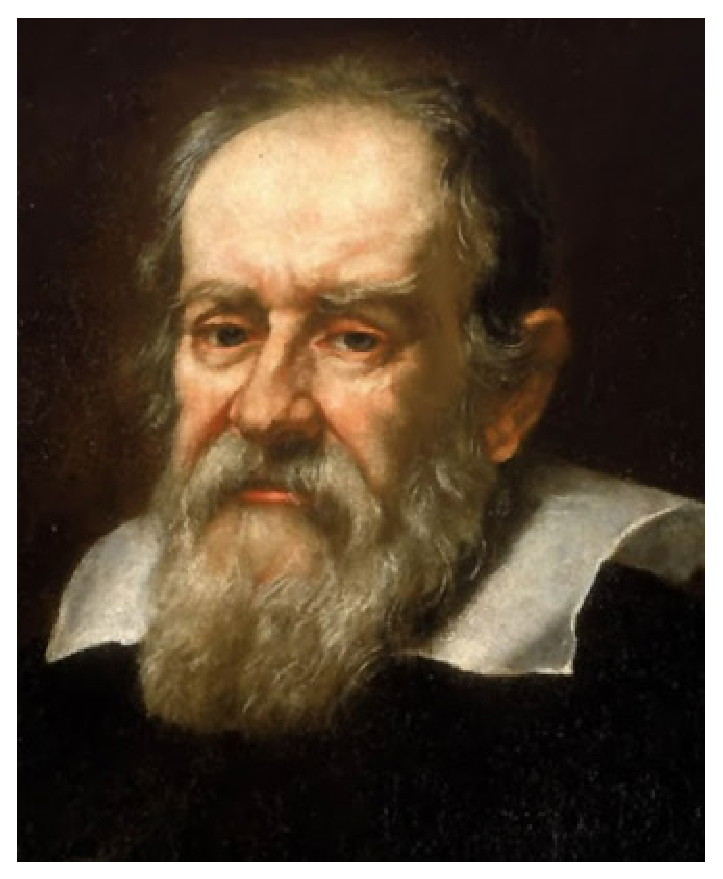
\includegraphics[scale=0.25]{Galilee.eps}\\
\emph{{\small Galileo Galilei}}\\
\href{http://fr.wikipedia.org/wiki/Galileo Galilei}{http://fr.wikipedia.org/wiki/Galileo Galilei}\\[5mm]
\end{center}



3034-- Christoff Rudolff a \'ecrit un trait\'e, \og \emph{Das Coss} \fg, pour \og \emph{la chose} \fg \ dans le sens de l'inconnu d'une \'equation alg\'ebrique. Quel symbole a invent\'e ce math\'ematicien allemand, en 1525?\\

a) ensemble vide :\ \ $\varnothing$\\
b) infini :\ \ $\infty$\\
c) ensemble des naturels :\ \ $\mathbb{N}$\\
d) racine carr\'ee :\ \ $\surd$\\

R\'eponse : d)\\

R\'etroaction :\\
La r\'esolution d'\'equations quadratiques fait intervenir la notion de racine carr\'ee. Les gens de l'\'epoque avaient donc besoin d'une notation pour exprimer cette op\'eration math\'ematique. Christoff Rudolff a \'etudi\'e la r\'esolution d'\'equation alg\'ebrique. Il a utilis\'e et invent\'e des notations aussi concises que possible, dont le symbole de racine carr\'ee ($\surd$). Donc la r\'eponse est d). De nos jours, on utilise le m\^eme symbole, mais avec la barre au dessus ($\sqrt{ \ \ }$).\\



%{\bf \textsf{animation : petit bonhhomme d\'eguis\'e en Harry Potter et qui vole sur son balai}}\\
3035-- Qui, \`a la fin du {\scriptsize I\ier{}} si\`ecle, a \'etabli une fa\c con d'approximer les racines carr\'ees pour n'importe quel nombre?\\

a) Harry Potter\\
b) H\'eron d'Alexandrie\\
c) J\'er\^ome Cardan\\
d) Pierre-Simon Laplace\\

R\'eponse : b)\\

R\'etroaction :\\
En plus de sa formule de H\'eron pour calculer l'aire d'un triangle quelconque, H\'eron d'Alexandrie a trouv\'e une formule pour approximer la racine carr\'ee de n'importe quel nombre. La r\'eponse est donc b).\\


% pas de niveau secondaire
%3036-- Quel concept math\'ematique a \'et\'e d\'efini par Augustin-Louis Cauchy, un math\'ematicien fran\c cais du 18\ieme si\`ecle et red\'efini plus tard par Eduard Heine, un math\'ematicien allemand du 19\ieme{} si\`ecle? (Heine trouvait que la d\'efinition de Cauchy n'\'etait pas assez claire et qu'elle pouvait \^etre plus pr\'ecise.)\\

%a) continuit\'e d'une fonction\\
%b) domaine d'une fonction\\
%c) fonction cosinus\\
%d) fonction sinus\\

%R\'eponse : a)\\

%R\'etoaction :\\
%Cauchy a centr\'e son travail en analyse math\'ematique (calcul infinit\'esimal). Ce domaine traite des concepts de fonction, de limite, de d\'eriv\'ee, d'int\'egrale et \`a prime \`a bord, de continuit\'e. La r\'eponse est a). En 1872, Heine a donn\'e la d\'efinition de la continuit\'e telle que les math\'ematiciens la connaissent aujourd'hui.\\ \includegraphics[scale=0.3]{Cauchy.eps} \includegraphics[scale=0.3]{Heine.eps}



3036-- Au Moyen-\^Age, qui, dans ses \'ecrits, a \'enonc\'e les r\`egles de transformations des \'equations?\\

a) Al-Khwarizmi\\
b) Jesuis Dumoi Ien\^age\\
c) Jean Bernoulli\\
d) Joseph-Louis Lagrange\\

R\'eponse : a)\\

R\'etroaction :\\
Al-Khwarizmi a \'ecrit \og \emph{Al-jabr wa'l-muqabalah} \fg, qui veut dire \og \emph{La transposition et la r\'eduction} \fg. Ce livre d\'ecrit en mots des fa\c cons de transformer des \'equations alg\'ebriques. La r\'eponse est a). Notons que \og \emph{al-jabr} \fg \ sera repris plus tard par les Europ\'eens pour nommer une branche des math\'ematiques : \og \emph{l'alg\`ebre} \fg.

\begin{center}
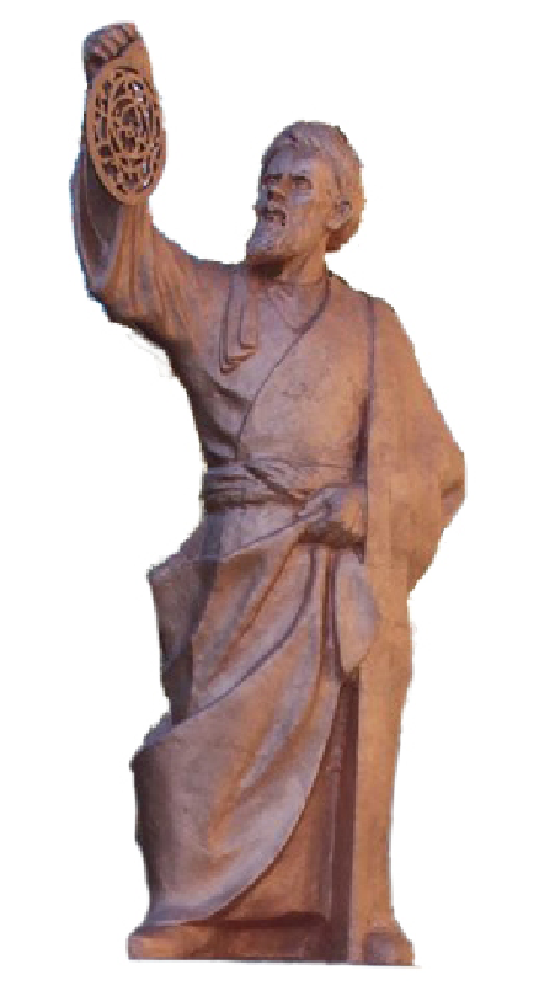
\includegraphics[scale=0.25]{Al-Khwarizmi.eps}\\
\emph{{\small Al-Khwarizmi}}\\
\href{http://fr.wikipedia.org/wiki/Al-Khwarizmi}{http://fr.wikipedia.org/wiki/Al-Khwarizmi}\\[5mm]
\end{center}


3037-- De quel sujet traite principalement \og \emph{Les \'El\'ements d'Euclide} \fg, \'ecrit par Euclide lui-m\^eme?\\

a) arithm\'etique\\
b) g\'eom\'etrie\\
c) optimisation\\
d) statistiques\\

R\'eponse : b)\\

R\'etroaction :\\
\og \emph{Les \'El\'ements d'Euclide} \fg \ est un recueil de connaissances g\'eom\'etriques de la Gr\`ece Antique, sujet d'\'etude principal des math\'ematiciens de l'\'epoque. Donc la r\'eponse est b). Le recueil se divise en 13 livres.\\
\begin{center}
\begin{tabular}{|c|c|} \hline
{\bf Num\'eros des livres} & {\bf Contenu} \\ \hline \hline
1 \`a 6 & g\'eom\'etrie plane \\ \hline
7 \`a 9 & th\'eorie des rapports \\ \hline
10 & th\'eorie des nombres irrationnels \\ \hline
11 \`a 13 & g\'eom\'etrie de l'espace \\ \hline
\multicolumn{2}{c}{}
\end{tabular}
\end{center}
Notons que la g\'eom\'etrie apprise au primaire et au secondaire est appel\'ee g\'eom\'etrie euclidienne. Il existe \'egalement d'autres types de g\'eom\'etrie, par exemple hyperbolique et sph\'erique.\\



3038-- Quel math\'ematicien fran\c cais a \'et\'e le premier \`a introduire le symbole \og$\angle$\fg pour nommer un angle?\\

a) Adrien-Marie Legendre\\
b) Breauch\`ete Depoulais\\
c) Charlie Brown\\
d) Pierre H\'erigone\\

R\'eponse : d)\\

R\'etroaction :\\
Pierre H\'erigone a introduit beaucoup de notations symboliques dans son trait\'e en six volumes, \og \emph{Un abr\'eg\'e de math\'ematiques \'el\'ementaires} \fg. Il a entre autres introduit le symbole pour la mesure de l'angle, \og$\angle$\fg. Donc la r\'eponse est d). (Il a \'egalement introduit le symbole \og$\perp$\fg \ pour exprimer le fait que deux droites sont perpendiculaires.)\\



3039-- Un probl\`eme math\'ematique est dit \emph{ouvert} lorsque sa solution est inconnue.\\
Dans les ann\'ees 1940, dans un cours au doctorat de l'Universit\'e de Berkeley, un professeur note au tableau deux probl\`emes ouverts en statistiques. Un \'etudiant en retard note ces probl\`emes croyant qu'il s'agit d'un devoir. Il les a r\'esolu en quelques jours seulement. De qui s'agit-il?\\

a) Bhaskara I\ier{}\\
b) Fo\^etre Ung\'eny\\
c) Georges Dantzig\\
d) Pythagore\\

R\'eponse : c)\\

R\'etroaction :\\
C'est Georges Dantzig, un math\'ematicien des \'Etats-Unis, qui a r\'esolu ces probl\`emes, alors qu'il croyait qu'ils \'etaient \`a faire en devoir. La r\'eponse est c). Par le fait m\^eme, il a d\'evelopp\'e, sans le savoir, une m\'ethode de r\'esolution de probl\`emes d'optimisation.\\

\begin{center}
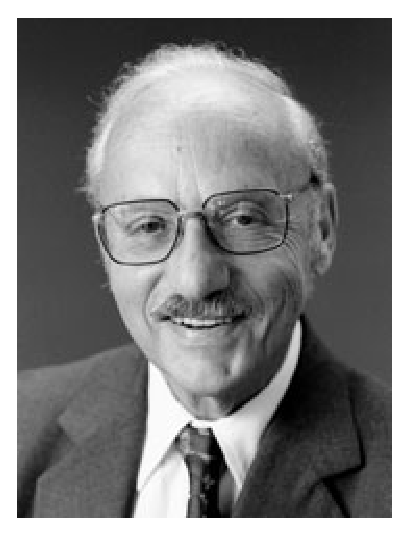
\includegraphics[scale=0.3]{dantzig.eps}\\
\emph{{\small Georges Dantzig}}\\
\href{http://www.siam.org/news/news.php?id=928}{www.siam.org/news/news.php?id=928}\\[5mm]
\end{center}



3040-- Selon la l\'egende, dans la Gr\`ece Antique, Thal\`es de Milet a \'et\'e mis au d\'efi par le Pharaon Amasis. Quel \'etait ce d\'efi?\\

a) Calculer le nombre de pi\`eces d'or qui pourraient entrer dans son sarcophage.\\
b) Concevoir un r\'eservoir d'eau assez grand pour alimenter la cit\'e pendant un mois.\\
c) D\'eterminer laquelle entre le Sphinx et la Grande Pyramide de Kh\'eops est la construction la plus lourde.\\
d) Mesurer la hauteur de la Grande Pyramide de Kh\'eops.\\

R\'eponse : d)\\

R\'etroaction :\\
Le Pharaon Amasis aurait dit que personne n'\'etait capable de mesurer la hauteur de la Grande Pyramide de Kh\'eops. La r\'eponse est donc d). Pour r\'eussir ce calcul, Thal\`es est parti du fait qu'\`a un certain moment de la journ\'ee, l'ombre de tout objet devient \'egale \`a la hauteur de l'objet lui-m\^eme (les rayons du soleil sont alors inclin\'es \`a 45$^\circ$). Il a d\'etermin\'e ce moment, pour une journ\'ee pr\'ecise, et il a utilis\'e sa propre grandeur pour mesurer l'ombre de la Grande Pyramide, \`a laquelle il a ajout\'e la moiti\'e de la mesure de la base de la pyramide. Il a obtenu 85 thal\`es, ce qui \'equivaut \`a 276,25 coud\'ees \'egyptiennes. En r\'ealit\'e, la pyramide mesure environ 280 coud\'ees \'egyptiennes (137 m\`etres) ce qui est une excellente approximation pour l'\'epoque.
\begin{center}
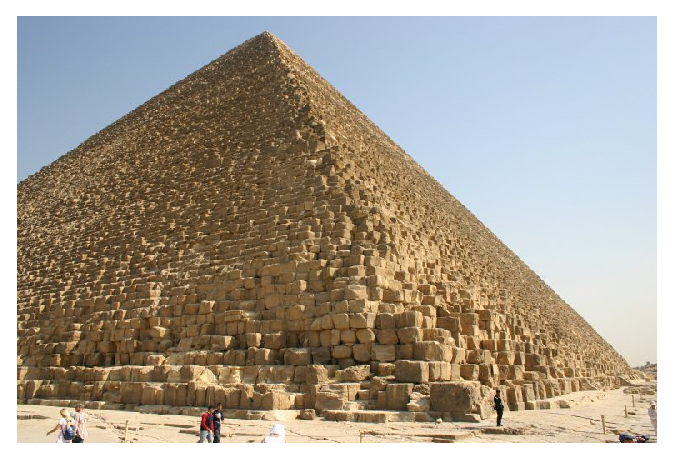
\includegraphics[scale=0.5]{pyramide.eps}\\
\emph{{\small Grande Pyramide de Kh\'eops}}\\
\href{http://fr.wikipedia.org/wiki/Pyramide de Kh\%C3\%A9ops}{fr.wikipedia.org/wiki/Pyramide de Kh\'eops}\\[5mm]
\end{center}



3041-- Jusqu'au {\scriptsize XIX\ieme{}} si\`ecle, les math\'ematiciens n'\'etaient pas appel\'es des math\'ematiciens. Quels noms leurs donnait-on?\\

a) arpenteurs\\
b) calculeurs\\
c) g\'eom\`etres\\
d) mesureurs\\

R\'eponse : c)\\

R\'etroaction :\\
Jusqu'au {\scriptsize XIX\ieme{}} si\`ecle, on appelait les math\'ematiciens des g\'eom\`etres. La r\'eponse est c). Comme au d\'epart les math\'ematiciens concentraient leurs recherches sur les calculs de volume, d'aire et de longueur, on les nomma des g\'eom\`etres. Par d\'efinition, un g\'eom\`etre est, entre autres, un arpenteur; il mesure des terres.\\



3042-- Il existe plusieurs types de g\'eom\'etrie : la g\'eom\'etrie euclidienne, hyperbolique, sph\'erique, \dots \ \ Qu'est-ce qui est \`a la base de toutes g\'eom\'etries, c'est-\`a-dire qu'est-ce qui d\'efinit une g\'eom\'etrie?\\

a) les figures que l'on peut tracer\\
b) les mesure des angles\\
c) le syst\`eme d'axiomes\\
d) le type de coordonn\'ees\\

R\'eponse : c)\\

R\'etroaction :\\
Les axiomes sont des r\`egles de base qui d\'efinissent une g\'eom\'etrie. La r\'eponse est c). Elles sont toujours vraies dans la g\'eom\'etrie qu'elles d\'efinissent, mais elles peuvent \^etre fausses dans une autre. Elles servent \`a d\'emontrer des th\'eor\`emes.\\



3043-- Historiquement, la g\'eom\'etrie euclidienne a \'et\'e invent\'ee en premier. Le dessin suivant:
\begin{center}
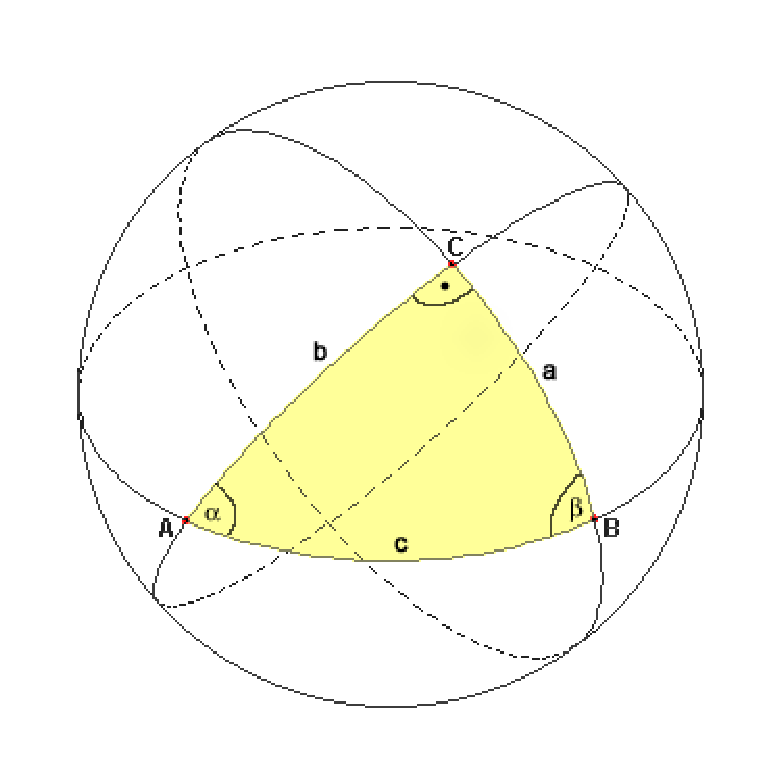
\includegraphics[scale=0.5]{geospher.eps}\\
\href{http://fr.wikipedia.org/wiki/Trigonom\%C3\%A9trie sph\%C3\%A9rique}{fr.wikipedia.org/wiki/}\\[5mm]
\end{center}
et l'axiome suivant : \og Il n'existe aucune droite qui passe par le point $A$ et qui soit parall\`ele \`a la droite $a$, c'est-\`a-dire que toutes les droites passant par le point $A$ coupent la droite $a$ \fg, d\'ecrivent quelle g\'eom\'etrie?\\

a) affine\\
b) hyperbolique\\
c) projective\\
d) sph\'erique\\

R\'eponse : d)\\

R\'etroaction :\\
Comme son nom l'indique, la g\'eom\'etrie sph\'erique est un ensemble de points et de droites sur une sph\`ere. La r\'eponse est d). On d\'efinit plus particuli\`erement un segment de droite comme le chemin le plus court entre deux points sur la sph\`ere.\\



3044-- Lequel parmi les math\'ematiciens suivants n'est pas consid\'er\'e comme l'un des plus grands g\'eom\`etres de l'Antiquit\'e?\\

a) Apollonius de Perge (262 - 180 avant J\'esus-Christ)\\
b) Archim\`ede de Syracuse (287 - 212 avant J\'esus-Christ)\\
c) Aristote (384 - 322 avant J\'esus-Christ)\\
d) Euclide (365 - 275 avant J\'esus-Christ)\\

R\'eponse : c)\\

R\'etroaction :\\
Apollonius de Perge est c\'el\`ebre pour ses \'ecrits sur les sections coniques.\\
\begin{center}
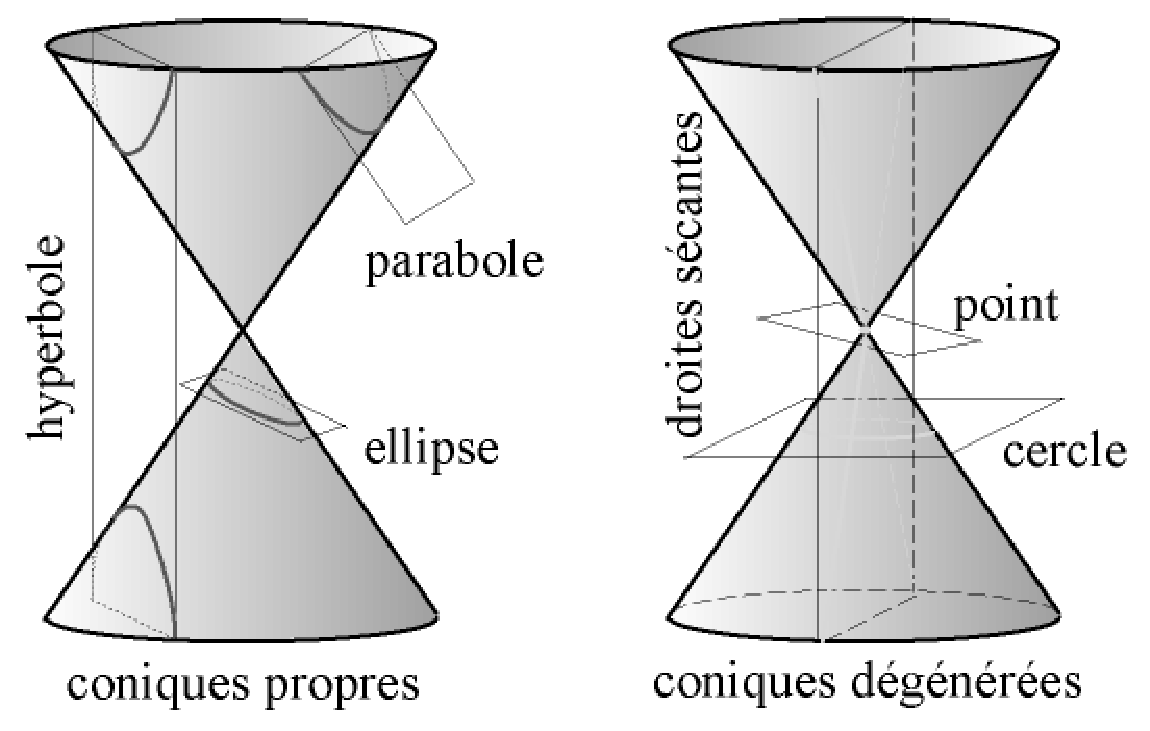
\includegraphics[scale=0.25]{Coniques.eps}\\
\emph{{\small Conique d'Apollonius}}\\
\href{http://fr.wikipedia.org/wiki/Coniques}{fr.wikipedia.org/wiki/Coniques}\\
\end{center}
Archim\`ede de Syracuse a \'etudi\'e les coniques, le calcul des aires et des volumes puis la spirale (spirale d'Archim\`ede).\\
\begin{center}
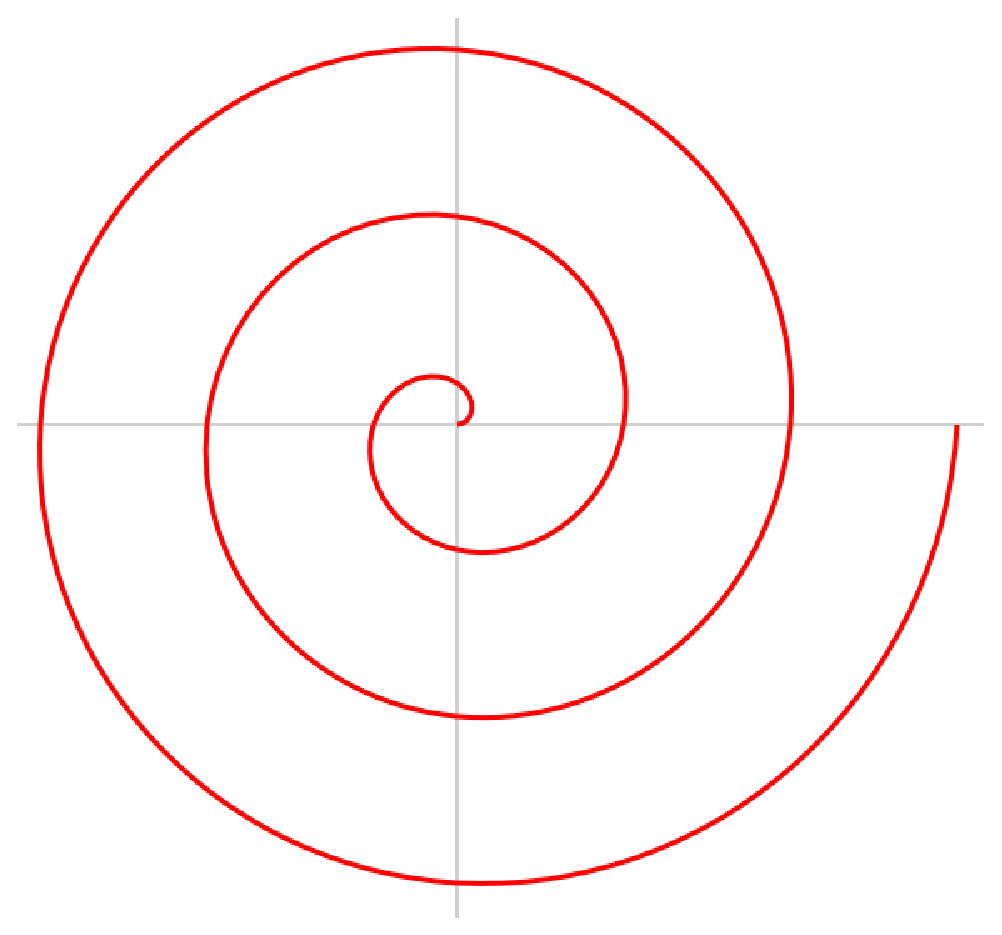
\includegraphics[scale=0.25]{spirale.eps}\\
\emph{{\small Spirale d'Archim\`ede}}\\
\href{http://fr.wikipedia.org/wiki/Spirale_d\%27Archim\%C3\%A8de}{fr.wikipedia.org/wiki/Spirale d'Archim\`ede}
\end{center}
%\emph{\textsf{animation qui montrerait la formation de la spirale}}\\
Aristote, qui \'etait un penseur, n'est pas consid\'er\'e comme un grand g\'eom\`etre de l'Antiquit\'e, mais plut\^ot comme un grand philosophe.  La r\'eponse est c).\\
Euclide est c\'el\`ebre pour son livre \og \emph{Les \'El\'ements d'Euclide} \fg, un recueil de connaissances g\'eom\'etriques.\\



3045-- Historiquement, le principal probl\`eme des math\'ematiciens concernant le nombre $\pi$ a \'et\'e de choisir un symbole pour le repr\'esenter.\\
Vrai ou Faux?\\

R\'eponse : Faux\\

R\'etroaction :\\
Le plus grand probl\`eme avec $\pi$ n'a pas \'et\'e de choisir quel symbole le repr\'esenterait, mais plut\^ot de trouver sa valeur. Beaucoup de math\'ematiciens ont cherch\'e et cherchent encore \`a d\'eterminer les d\'ecimales exactes de $\pi$. La r\'eponse est donc : faux. En septembre 2002, on d\'enombrait $1 \, 241 \, 100 \, 000 \, 000$ de d\'ecimales!\\
\begin{center}
\begin{tabular}{|c|c|c|c|} \hline
{\bf Nom} & {\bf Ann\'ee} & {\bf Nombre de d\'ecimales exactes de $\pi$} \\ \hline \hline
Babyloniens & -2000 & 1 \\ \hline
\'Egyptiens & -1650 & 1 \\ \hline
Chinois & -1200 & 0 \\ \hline
Archim\`ede & -250 & 3 \\ \hline
Ptol\'em\'ee & 150 & 3 \\ \hline
Al-Khwarizmi & 800 & 3 \\ \hline
Fran\c cois Viete & 1593 & 9 \\ \hline
John Machin & 1706 & 100 \\ \hline
Rutherford & 1853 & 440 \\ \hline
Nicholson et Jeenel & 1945 & 3092 \\ \hline
Guilloud et Bouyer & 1973 & $1 \, 001 \, 250$ \\ \hline
Kanada & 2002 & $1 \, 241 \, 100 \, 000 \, 000$\\ \hline
\end{tabular}\\[2mm]
Donn\'ees prises sur le site internet : \href{http://www.pi314.net/historique.php}{http://www.pi314.net/historique.php}\\[5mm]
\end{center}
%{\bf \textsf{animation : petit bonhomme \'ebahit, \'etourdit par le nombre de d\'ecimales}}\\



3046-- En 1765, le math\'ematicien allemand Johann Heinrich Lambert a d\'emontr\'e une propri\'et\'e de $\pi$. Quelle est-elle?\\

a) $\pi = 3,1416$\\
b) $\pi$ est un nombre irrationnel\\
c) $\pi$ est un nombre rationnel\\
d) $\pi$ poss\`ede un nombre fini, mais tr\`es grand, de d\'ecimales\\

R\'eponse : b)\\

R\'etroaction :\\
Johann Heinrich Lambert a prouv\'e que $\pi$ est irrationnel, c'est-\`a-dire qu'il n'existe pas de notation d\'ecimale exacte de $\pi$, il existe seulement des approximations. La r\'eponse est b).\\
\begin{center}
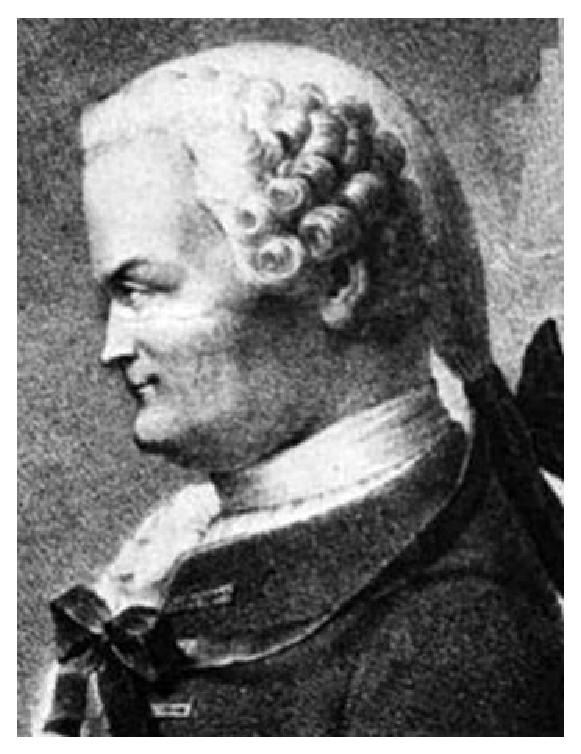
\includegraphics[scale=0.25]{JHLambert.eps}\\
\emph{{\small Johann Heinrich Lambert}}\\
\href{http://fr.wikipedia.org/wiki/Johann Heinrich Lambert}{fr.wikipedia.org/wiki/Johann Heinrich Lambert}\\[5mm]
\end{center}



3047-- Quel math\'ematicien anglais a \'et\'e le premier \`a utiliser la lettre grecque $\pi$ pour nommer ce nombre: 3,141 592 654 \dots ?\\

a) Apollonius de Perge\\
b) Scipione del Ferro\\
c) Sun Zi\\
d) William Jones\\

R\'eponse : d)\\

R\'etroaction :\\
En 1706, William Jones propose dans son ouvrage \og \emph{A New Introduction to the Mathematics} \fg \ d'utiliser le symbole $\pi$ pour repr\'esenter le rapport de la circonf\'erence d'un cercle sur son diam\`etre :
\begin{eqnarray*}
\pi &=& \frac{\textrm{circonf\'erence}}{\textrm{diam\`etre}}\\[2mm]
 &=& \frac{2\pi r}{d}\\[2mm]
 &=& \frac{d\pi}{d}
\end{eqnarray*}
Donc, la r\'eponse est d). Leonhard Euler a utilis\'e ce symbole en 1748 dans un de ses ouvrages.

\begin{center}
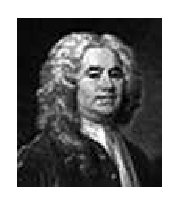
\includegraphics[scale=1]{William_Jones.eps}\\
\emph{{\small William Jones}}\\
\href{http://fr.wikipedia.org/wiki/William Jones \%28math\%C3\%A9maticien\%29}{fr.wikipedia.org/wiki/William Jones (mathematicien)}\\[5mm]
\end{center}



3048-- Vers quels si\`ecles est apparue la loi des exposants: \ $x^{m+n} = x^{m} \cdot x^{n}$ ?\\

a) {\scriptsize VI\ieme{}} et {\scriptsize V\ieme{}} si\`ecles\\
b) {\scriptsize XI\ieme{}} et {\scriptsize XII\ieme{}} si\`ecles\\
c) {\scriptsize XIV\ieme{}} et {\scriptsize XV\ieme{}} si\`ecles\\
d) {\scriptsize XXI\ieme{}} et {\scriptsize XXII\ieme{}} si\`ecles\\

R\'eponse : b)\\

R\'etroation :\\
Les Arabes ont invent\'e la loi des exposants entre les ann\'ees 1000 et 1200, soit vers le {\scriptsize XI\ieme{}} si\`ecle et le {\scriptsize XII\ieme{}} si\`ecle. La r\'eponse est b). Les Arabes \'ecrivaient leurs \'equations alg\'ebriques en mots et non pas en symboles.\\



3049-- Qui ont invent\'e l'algorithme de division des polyn\^omes?\\
Par exemple,
\begin{center}
\begin{tabular}{r}
$x^{2} - 1$ \ \ \ \ \ \ \\
\underline{$- (x^{2} + x)$} \ \ \ \  \ \\
$- x - 1$ \ \\
\underline{$- (-x - 1)$}\\
$0$ \
\end{tabular}
\begin{tabular}{|c}
$x + 1$ \\ \hline
$x - 1$\\
\\
\\
\\
\end{tabular}
\end{center}
%\textsf{animation : bonhomme pourrait effectuer la division??}\\

a) Arabes\\
b) Chinois\\
c) Fran\c cais de la Renaissance\\
d) Italiens de la Renaissance\\

R\'eponse : a)\\

R\'etroaction :\\
Dans les ann\'ees 1000-1200, ce sont les Arabes qui ont invent\'e l'algorithme de division des polyn\^omes. La r\'eponse est a). Ils ont d\'evelopp\'e la m\'ethode jusqu'\`a des puissances n\'egatives:\\
\begin{center}
\begin{tabular}{r}
$x^{2} + 1$ \ \ \ \ \ \ \ \ \ \ \ \ \ \ \ \ \ \ \ \ \ \ \ \\
\underline{$- (x^{2} + 2x)$} \ \ \ \ \ \ \ \ \ \ \ \ \ \ \ \ \ \ \ \ \\
$- 2x + 1$ \ \ \ \ \ \ \ \ \ \ \ \ \ \ \ \\
\underline{$- (-2x - 4)$} \ \ \ \ \ \ \ \ \ \ \ \ \ \ \\
$5$ \ \ \ \ \ \ \ \ \ \ \ \ \ \ \ \\
\underline{$- (5 + 10/x)$} \ \ \ \ \\
$-10/x$ \ \ \ \ \ \\
$\vdots$ \ \ \ \ \ \ \ \ \ \
\end{tabular}
\begin{tabular}{|c}
$x + 2$ \\ \hline
$x - 2 + 5/x - 10/x^{2} \cdots$\\
\\
\\
\\
\\
\\
\\

\end{tabular}\\
\end{center}



3050-- Al-Khwarizmi peut \^etre consid\'er\'e comme le p\`ere de l'alg\`ebre. Dans son livre \og \emph{al-jabr wa'l muqabala} \fg, il utilise le mot \og \emph{shai} \fg, chose, pour indiquer une variable. Lequel parmi les mots suivants n'a jamais \'et\'e utilis\'e pour d\'esigner une variable?\\

a) causa\\
b) cosa\\
c) cose\\
d) coss\\

R\'eponse : c)\\

R\'etroaction :\\
Quelques textes en latin utilisent le mot \og \emph{causa} \fg \ pour le mot \og \emph{shai} \fg \ d'Al-Khwarizmi. Traduit en italien, \og \emph{causa} \fg \ devient \og \emph{cosa} \fg \ et en allemand, \og \emph{coss} \fg. \og \emph{Cose} \fg \ n'a jamais \'et\'e utilis\'e pour indiquer une variable. La r\'eponse est c).\\



3051--
\begin{center}
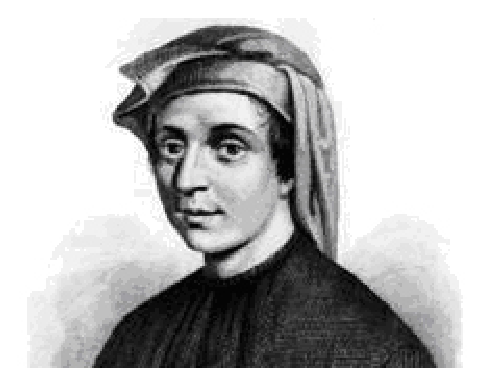
\includegraphics[scale=0.4]{Fibonacci.eps}\\
\emph{{\small L\'eonard de Pise {\scriptsize dit} Fibonacci}}\\
\href{http://fr.wikipedia.org/wiki/Fibonacci}{fr.wikipedia.org/wiki/Fibonacci}\\
\end{center}

\`A l'\'epoque de L\'eonard de Pise (1170-1250), une \'equation alg\'ebrique s'\'ecrivait encore en mots. Soit l'expression suivante:\\
\begin{quote}
\og \emph{Le cube et 8 choses moins 5 carr\'ees est \'egale \`a la racine de 1 de plus qu'une chose.} \fg\\
\end{quote}
Comment l'\'ecrirait-on de nos jours?\\

a) $x^{3} - 5x^{2} + 8 = \sqrt{x} + 1$\\[2mm]
b) $x^{3} - 5x^{2} + 8 = \sqrt{x + 1}$\\[2mm]
c) $x^{3} - 5x^{2} + 8x = \sqrt{x} + 1$\\[2mm]
d) $x^{3} - 5x^{2} + 8x = \sqrt{x + 1}$\\

R\'eponse : d)\\

%\emph{\textsf{animation : petit bonhomme d\'eguis\'e en magicien, prend chaque expression en mots et la transforme en symbole}}\\
R\'etroaction :\\
\begin{center}
\begin{tabular}{|c|c|}\hline
Le cube & $x^{3}$\\ \hline
et & $+$\\ \hline
8 choses & $8x$\\ \hline
moins 5 carr\'ees & $-5x^{2}$\\ \hline
est \'egale \`a & $=$\\ \hline
la racine de 1 de plus qu'une chose & $\sqrt{x + 1}$\\ \hline
\end{tabular}\\[4mm]
$\Longrightarrow \ \ \ \ \ \ \ x^{3} + 8x - 5x^{2} = \sqrt{x + 1} \ \ \ \ \ \ \ \Longleftrightarrow \ \ \ \ \ \ \ x^{3} - 5x^{2} + 8x = \sqrt{x + 1}$
\end{center}
Donc, la r\'eponse est d).\\


3052-- Comment les Anglais appelaient-ils l'\'etude des \'equations alg\'ebriques?

a) \og \emph{Art of The Thing} \fg\\
b) \og \emph{Cossic Art} \fg\\
c) \og \emph{Equations Art} \fg\\
d) \og \emph{The Thing and its Art} \fg\\

R\'eponse : b)\\

R\'etroaction :\\
L'\'ecriture des \'equations alg\'ebriques se faisait avec des mots et non avec des symboles; elle \'etait tr\`es complexe et on la consid\'erait comme un art. Les Anglais se sont inspir\'es du mot \og \emph{coss} \fg, chose, qui d\'esignait une variable pour les math\'ematiciens allemands, \og \emph{coss} \fg, \og \emph{cossic} \fg, d'o\`u son nom : \og \emph{Cossic Art} \fg. La r\'eponse est b).\\



3053-- En quelle ann\'ee le livre \og \emph{Summa Aritmetica} \fg, du moine italien Luca Pacioli, est-il paru?\\

a) 1494\\
b) 1724\\
c) 1894\\
d) 2006\\

\begin{center}
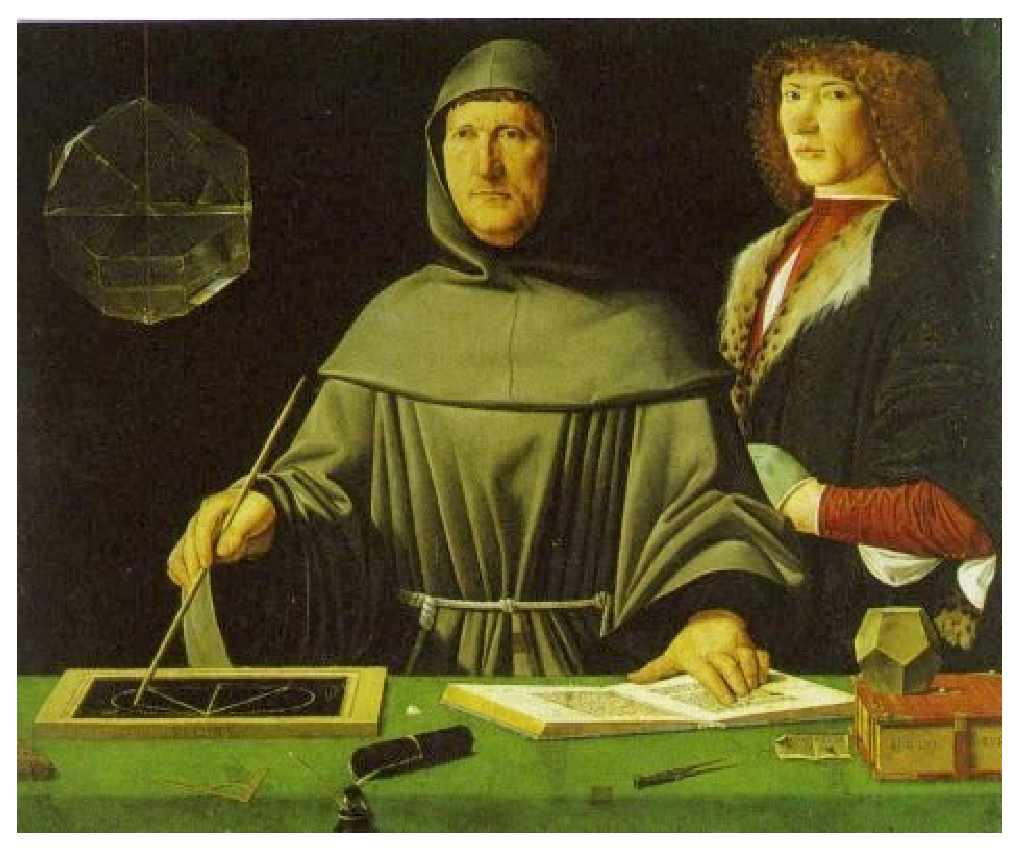
\includegraphics[scale=0.25]{Pacioli.eps}\\
\emph{{\small Luca Pacioli}}\\
\href{http://fr.wikipedia.org/wiki/Luca Pacioli}{fr.wikipedia.org/wiki/Luca Pacioli}\\
\end{center}

R\'eponse : a)\\

R\'etroaction :\\
\og \emph{Summa Aritmetica} \fg \ paru en 1494. La r\'eponse est a). Ce livre servira de principale source d'introduction de la symbolique de l'art des expressions alg\'ebriques.\\



3054-- Le principal probl\`eme avec la notation de Luca Pacioli est qu'on peut exprimer, dans une \'equation alg\'ebrique, une seule inconnue \`a la fois. Une telle \'equation serait de la forme :\\
\begin{eqnarray*}
cu.\tilde{m}.5.ce.\tilde{p}.7.co.\textrm{------}\mathcal{R}v.co.\tilde{p}.6.
\end{eqnarray*}
Vrai ou Faux?\\

R\'eponse : Vrai\\

R\'etroaction :\\
\begin{eqnarray*}
cu.\tilde{m}.5.ce.\tilde{p}.7.co.\textrm{------}\mathcal{R}v.co.\tilde{p}.6.
\end{eqnarray*}
L'abbr\'eviation \og $co$ \fg \ est pour \og \emph{cosa} \fg, chose, la quantit\'e inconnue. \og $ce$ \fg \ et \og $cu$ \fg \ sont respectivement \og \emph{censo} \fg  \ et \og \emph{cubo} \fg, de l'italien carr\'e et cube. \og $v$ \fg \ veut dire \og \emph{universel} \fg. Il regroupe les termes qui le suivent. Comme \og \emph{co} \fg \ r\'ef\`ere \`a une seule quantit\'e inconnue, la faiblesse de cette notation est l'impossibilit\'e de repr\'esenter plus d'une inconnue \`a la fois. La r\'eponse est : vrai. En notation actuelle, l'expression s'\'ecrirait:\\
\begin{eqnarray*}
cu.\tilde{m}.4.ce.\tilde{p}.10.co.\textrm{------}\mathcal{R}v.co.\tilde{p}.3. \ \ \Longleftrightarrow \ \ x^{3} - 4x^{2} + 10x = \sqrt{x + 3}
\end{eqnarray*}\\



3055-- En 1484, quel math\'ematicien fran\c cais a cr\'e\'e sa propre notation pour les expressions alg\'ebriques et pour les exposants?\\

a) Beno\^it Mandelbrot\\
b) Bob Barker\\
c) Joseph Liouville\\
d) Nicolas Chuquet\\

R\'eponse : d)\\

R\'etroation :\\
Nicolas Chuquet a \'ecrit \og \emph{Triparty en la science des nombres} \fg, un livre qui traite de l'alg\`ebre. Il y cr\'ee des notations dans le but de clarifier l'art de travailler avec les expressions alg\'ebriques.  Il introduit des termes tels que :\\
\begin{eqnarray*}
5^{2} \ \ \ \ \ \text{qui s'\'ecrit maintenant:} \ \ \ \ \ 5x^{2}.\\
\mathcal{R}^{3} 5 \ \ \ \ \ \text{qui s'\'ecrit maintenant:} \ \ \ \ \ \sqrt[3]{5}.
\end{eqnarray*}
La r\'eponse est d).\\



3056-- Nicolas Chuquet n'a jamais publi\'e son livre \og \emph{Triparty en la science des nombres} \fg \ de son vivant. Un de ses \'el\`eve a publi\'e \og \emph{L'arismetique} \fg \ qui est en fait une copie du livre de Chuquet. Qui est ce math\'ematicien fran\c cais \og copieur \fg ?\\

a) Atomic Betty\\
b) Estienne de La Roche\\
c) Pythagore\\
d) Ren\'e Descartes\\

R\'eponse : b)\\

%\emph{\textsf{animation : p'tit bonhommme pourrait passer, d\'eguis\'e en voleur, avec un livre sous le bras...}}\\
R\'etroaction :\\
C'est Estienne de La Roche qui a publi\'e \og \emph{L'arismetique} \fg, une copie de \og \emph{Triparty en la science des nombres} \fg, en 1520. La r\'eponse est b). C'est seulement en 1880 que l'oeuvre de Chuquet est publi\'e officiellement pour la premi\`ere fois.\\



3057-- \`A quel math\'ematicien fran\c cais doit-on le syst\`eme des grands nombres suivant?\\
\begin{center}
\begin{tabular}{|c|c|c|c|} \hline
{\bf Base 10} & {\bf Puissance} & {\bf Nom donn\'e par \dots} & {\bf Notation de \dots} \\ \hline \hline
$10^{0}$ & million$^{0}$ & unit\'e & 1\\[1mm] \hline
$10^{3}$ & million$^{0.5}$ & mille & 1000\\[1mm] \hline
$10^{6}$ & million$^{1}$ & million & 100000\\[1mm] \hline
$10^{9}$ & million$^{1.5}$ & mille million & 100.000000\\[1mm] \hline
$10^{12}$ & million$^{2}$ & billion & 100000.000000\\[1mm] \hline
$10^{15}$ & million$^{2.5}$ & mille billion & 100.000000.000000\\[1mm] \hline
$10^{18}$ & million$^{3}$ & trillion & 100000.000000.000000\\[1mm] \hline
\multicolumn{4}{c}{}\\
\end{tabular}\\
\end{center}
Cette premi\`ere notation utilise les points pour s\'eparer un grand nombre en paquets de six chiffres. De nos jours, en notation fran\c caise, on utilise des espaces pour s\'eparer un grand nombre en paquets de trois chiffres au lieu d'en paquets de six. Les anglais utilisent encore le point pour s\'eparer un grand nombre, mais en paquets de trois chiffres.\\

a) Blaise Pascal\\
b) Joseph Liouville\\
c) Nicolas Chuquet\\
d) Pafnouti Tchebychev\\

R\'eponse : c)\\

R\'etroaction :\\
Nicolas Chuquet a eu l'id\'ee de grouper les grands nombres en paquets de six chiffres qu'il s\'eparait par des points. La r\'eponse est c). C'est au d\'ebut du {\scriptsize XVII\ieme{}} si\`ecle, pour une meilleure lisibilit\'e, que l'on a divis\'e les grands nombres en groupes de trois au lieu de six. De nos jours, on utilise les espaces au lieu des points (les anglais, par contre, utilisent encore les points).\\
\begin{center}
\begin{tabular}{|c|c|c|c|} \hline
{\bf Base 10} & {\bf Puissance} & {\bf Nom donn\'e par Chuquet} & {\bf Notation de Chuquet} \\ \hline \hline
$10^{0}$ & million$^{0}$ & unit\'e & 1\\[1mm] \hline
$10^{3}$ & million$^{0.5}$ & mille & 1000\\[1mm] \hline
$10^{6}$ & million$^{1}$ & million & 100000\\[1mm] \hline
$10^{9}$ & million$^{1.5}$ & mille million & 100.000000\\[1mm] \hline
$10^{12}$ & million$^{2}$ & billion & 100000.000000\\[1mm] \hline
$10^{15}$ & million$^{2.5}$ & mille billion & 100.000000.000000\\[1mm] \hline
$10^{18}$ & million$^{3}$ & trillion & 100000.000000.000000\\[1mm] \hline
\multicolumn{4}{c}{}\\
\end{tabular}\\
\end{center}



3058-- Quel math\'ematicien fran\c cais a propos\'e des noms uniques pour les groupements de grands nombres \`a trois chiffres?\\
\begin{center}
\begin{tabular}{|c|c|c|} \hline
{\bf Base 10} & {\bf Puissance} & {\bf Nom donn\'e par Peletier du Mans} \\ \hline \hline
$10^{0}$ & million$^{0}$ & unit\'e \\[1mm] \hline
$10^{3}$ & million$^{0.5}$ & mille \\[1mm] \hline
$10^{6}$ & million$^{1}$ & million \\[1mm] \hline
$10^{\bf{9}}$ & million$^{\bf{1.5}}$ & \textbf{milliard} \\[1mm] \hline
$10^{12}$ & million$^{2}$ & billion \\[1mm] \hline
$10^{\bf{15}}$ & million$^{\bf{2.5}}$ & \textbf{billiard} \\[1mm] \hline
$10^{18}$ & million$^{3}$ & trillion \\[1mm] \hline
$10^{\bf{21}}$ & million$^{\bf{3.5}}$ & \textbf{trilliard} \\[1mm] \hline
\multicolumn{3}{c}{}\\
\end{tabular}\\
\end{center}

a) Isaac Newton\\
b) Jacques Peletier du Mans\\
c) Nicolas Chuquet\\
d) William Brouncker\\

R\'eponse : b)\\

R\'etroaction :\\
Jacques Peletier du Mans a propos\'e des noms pour les grands nombres interm\'ediaires (\`a trois chiffres). La r\'eponse est b).
\begin{center}
\begin{tabular}{|c|c|c|} \hline
{\bf Base 10} & {\bf Puissance} & {\bf Nom donn\'e par Peletier du Mans} \\ \hline \hline
$10^{0}$ & million$^{0}$ & unit\'e \\[1mm] \hline
$10^{3}$ & million$^{0.5}$ & mille \\[1mm] \hline
$10^{6}$ & million$^{1}$ & million \\[1mm] \hline
$10^{\bf{9}}$ & million$^{\bf{1.5}}$ & \textbf{milliard} \\[1mm] \hline
$10^{12}$ & million$^{2}$ & billion \\[1mm] \hline
$10^{\bf{15}}$ & million$^{\bf{2.5}}$ & \textbf{billiard} \\[1mm] \hline
$10^{18}$ & million$^{3}$ & trillion \\[1mm] \hline
$10^{\bf{21}}$ & million$^{\bf{3.5}}$ & \textbf{trilliard} \\[1mm] \hline
\multicolumn{3}{c}{}\\
\end{tabular}\\
\end{center}



3059-- Dans les ann\'ees 1600, plusieurs math\'ematiciens ont \'etabli des notations symboliques pour les expressions alg\'ebriques. Associe chaque math\'ematicien \`a la notation qu'il a invent\'ee?\\
\begin{center}
\begin{tabular}{|c|c|} \cline{2-2}
\multicolumn{1}{c|}{} & \multicolumn{1}{|c|}{\bf Notation}\\ \hline
1) & $4aaa + 7ee$\\ \hline
2) & $4a3 + 7e2$\\ \hline
3) & $4a^{iii} + 7e^{ii}$\\ \hline
4) & $4a^{3} + 7e^{2}$\\ \hline
\end{tabular} \ \ \ \ \ \ \ \
\begin{tabular}{|c|l|} \cline{2-2}
\multicolumn{1}{c|}{} & \multicolumn{1}{|c|}{\bf Math\'ematicien}\\ \hline
A) & 1620 - Thomas Harriot\\ \hline
B) & 1634 - Pierre H\'erigone\\ \hline
C) & 1636 - James Hume\\ \hline
D) & 1637 - Ren\'e Descartes\\ \hline
\end{tabular}
\end{center}

a) 1-A; 2-B; 3-C; 4-D\\
b) 1-B; 2-C; 3-A; 4-D\\
c) 1-C; 2-A; 3-D; 4-B\\
d) 1-D; 2-C; 3-A; 4-D\\

R\'eponse : a)\\

%{\bf \textsf{animation: petit bonhomme pourrait \^etre comme la miss Roue de Fortune et d\'evoiler les bonnes r\'eponses}}\\
R\'etroaction :\\
\begin{center}
\begin{tabular}{|c|c|l|} \cline{2-3}
\multicolumn{1}{c|}{} & \multicolumn{1}{|c|}{\bf Notation} & \multicolumn{1}{|c|}{\bf Math\'ematicien}\\ \hline
1-A & $4aaa + 7ee$ & 1620 - Thomas Harriot\\ \hline
2-B & $4a3 + 7e2$ & 1634 - Pierre H\'erigone\\ \hline
3-C & $4a^{iii} + 7e^{ii}$ & 1636 - James Hume\\ \hline
4-D & $4a^{3} + 7e^{2}$ & 1637 - Ren\'e Descartes\\ \hline
\end{tabular}\\
\end{center}
La r\'eponse est a).\\



3060-- Quel math\'ematicien fran\c cais du {\scriptsize XVII\ieme{}} si\`ecle a introduit l'utilisation des premi\`eres lettres de l'alphabet pour les constantes $(a,\,b,\,c,\,\dots)$ et les derni\`eres lettres pour les inconnues ($x,\,y,\,z$)?\\

a) Bartholomew J. Simpson\\
b) Galileo Galilei\\
c) Pierre Fatou\\
d) Ren\'e Descartes\\

R\'eponse : d)\\

R\'etroaction :\\
En plus d'avoir introduit la notation suivante : $5x^{3} - 8y^{2}$, c'est-\`a-dire les exposants pour exprimer les puissances, Ren\'e Descartes a introduit l'utilisation des lettres de l'alphabet: les constantes, par les premi\`eres lettres ($a, b, c, \dots$) et les inconnues, par les derni\`eres ($x, y, z$). La r\'eponse est d).\\
\begin{center}
\includegraphics[scale=0.4]{Descartes.eps}\\
\emph{{\small Ren\'e Descartes}}\\
\href{http://fr.wikipedia.org/wiki/Ren\%C3\%A9 Descartes}{fr.wikipedia.org/wiki/Ren\'e Descartes}\\[5mm]
\end{center}



3061-- Quel math\'ematicien britannique du {\scriptsize XVI\ieme{}} si\`ecle a introduit le signe d'\'egalit\'e ($=$) tel qu'on le conna\^it aujourd'hui?\\

a) Bonaventura Cavalieri\\
b) Danny Oc\'ean\\
c) Robert Recorde\\
d) Sofia Kovalevska\"ia\\

R\'eponse : c)\\

R\'etroaction :\\
En 1557, Robert Recorde a propos\'e l'utilisation du signe \og$=$\fg \ pour d\'esigner l'\'egalit\'e. La r\'eponse est c). Ce symbole \'etait tr\`es utilis\'e en Angleterre, mais tr\`es peu populaire en Europe continentale. C'est Isaac Newton et Gottfried Wilhelm von Leibniz qui ont probablement le plus contribu\'e \`a l'adoption du symbole \og$=$\fg.\\
\begin{center}
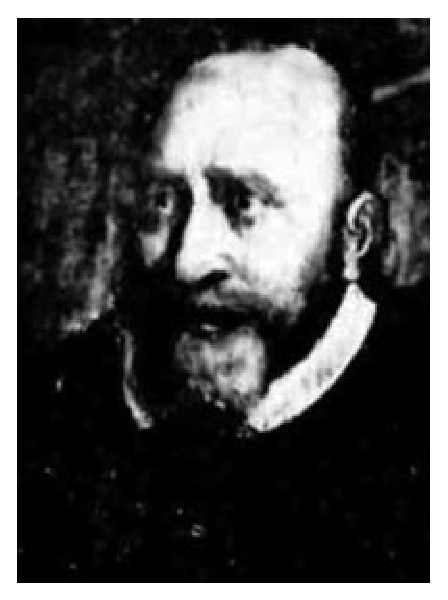
\includegraphics[scale=0.4]{recorde.eps}\\
\emph{{\small Robert Recorde}}\\
\href{http://www.pbs.org/wgbh/nova/einstein/ance-equals.html}{www.pbs.org/wgbh/nova/einstein/ance-equals.html}\\[5mm]
\end{center}



3062-- Quel symbole n'a jamais \'et\'e utilis\'e pour repr\'esenter l'\'egalit\'e ($=$)?\\

a) \includegraphics[scale=0.09]{egaliteDescartes.eps}\\
b) $\sim$\\
c) ------\\
d) $\asymp$\\

R\'eponse : d)\\

R\'etroaction :\\
Ren\'e Descartes a introduit \includegraphics[scale=0.09]{egaliteDescartes.eps}. Pacioli utilisait le symbole ------. Dans des ouvrages du {\scriptsize XVII\ieme{}} si\`ecle, on retrouve parfois le symbole $\sim$ (de nos jours, $\sim$ d\'esigne une approximation). Mais $\asymp$ n'a jamais \'et\'e utilis\'e pour d\'esigner l'\'egalit\'e. La r\'eponse est d).\\



3063-- En \'Egypte Antique, les scribes r\'esolvaient d\'ej\`a des \'equations du premier degr\'e. Par exemple :
\begin{center}
\og \emph{Une quantit\'e; son tiers plus lui-m\^eme devient 16.} \fg\\
\end{center}
En notation actuelle, on \'ecrirait : $x + \frac{x}{3} = 16$.\\[2mm]
Les scribes proc\'edaient ainsi :\\
\begin{itemize}
\item Ils choisissaient une quantit\'e; ici ce serait 3, car le tiers de 3 est facile \`a calculer! \ ($3\times \frac{1}{3} = 1$)
\item 3 plus le tiers de 3 devient $3 + \frac{3}{3} = 3 + 1 = 4$.
\item On veut 16, mais on a 4. On doit multiplier par 4. ($4 \times 4 = 16$).
\item Comme $x = 3$, alors $4 \times 3 = 12$.\\
La r\'eponse est 12.
\end{itemize}
V\'erification : si $x = 12$, alors $x + \frac{x}{3} = 12 + \frac{12}{3} = 12 + 4 = 16$.\\
\\
Quel nom porte cette m\'ethode?\\

a) m\'ethode de la division compl\'ementaire\\
b) m\'ethode de la fausse position\\
c) m\'ethode de la multiplication compl\`ete\\
d) m\'ethode de la substitution\\

R\'eponse : b)\\

R\'etroaction :\\
Cette m\'ethode porte le nom de fausse position, car on choisit un premier $x$ duquel on ne s'attend pas \`a avoir une bonne r\'eponse, mais qui se manipule facilement. La r\'eponse est b). On ram\`ene l'expression sous la forme $Ax = B$. Il para\^it facile de r\'esoudre cette \'equation, mais il faut se rappeler qu'\`a l'\'epoque, le calcul fractionnaire et le symbolisme n'\'etait pas tout \`a fait au point et que les nombres n\'egatifs n'\'etaient pas encore invent\'es.\\



3064-- La m\'ethode de la double fausse position permet de calculer une \'equation du premier degr\'e de la forme $Ax + C = B$. Quel peuple a invent\'e cette m\'ethode?\\

a) Arabes\\
b) Babyloniens\\
c) Chinois\\
d) \'Egyptiens\\

R\'eponse : c)\\

R\'etroaction :\\
Les Chinois ont d\'evelopp\'e la m\'ethode de la double fausse position pour pouvoir r\'esoudre des \'equations du premier degr\'e de la forme $Ax + C = B$. La r\'eponse est c). Notons que les Indiens utilisaient \'egalement cette m\'ethode.\\



3065-- Pour r\'esoudre une \'equation quadratique ($ax^{2} + bx + c = 0$), le math\'ematicien Al-Khwarizmi utilisait la formule suivante:
\begin{eqnarray*}
x = \sqrt{\Big(\frac{b}{2}\Big)^{2} + c} \ - \frac{b}{2}
\end{eqnarray*}
En fait, Al-Khwarizmi \'etudiait l'\'equation de la forme $x^{2} + bx = c$, o\`u les constantes $b$ et $c$ sont positives. Notons que cette notation n'existait pas \`a l'\'epoque et qu'elle aurait \'et\'e \'ecrite en mots.\\

La plus grande diff\'erence entre cette formule et celle que l'on conna\^it aujourd'hui
\begin{eqnarray*}
x = \frac{-b \pm \sqrt{b^{2} - 4ac}}{2a}
\end{eqnarray*}
est seulement la fa\c con de l'\'ecrire.\\
Vrai ou Faux?\\

R\'eponse: Faux\\

R\'etroaction :\\
\`A l'\'epoque, les gens ne consid\'eraient que les racines positives et rejetaient les racines n\'egatives, car ils ne connaissaient pas encore les nombres n\'egatifs. De nos jours, on consid\`ere les deux racines, d'o\`u l'apparition du $\pm$. Ainsi, la plus grande diff\'erence entre ces deux formules n'est pas dans la fa\c con de les \'ecrire, mais dans le fait que l'on consid\`ere deux racines. La r\'eponse est : faux.\\



%trop longue
%3066-- Soit l'\'equation quadratique suivante:
%\begin{eqnarray}
%x^{2} + 8x = 20
%\end{eqnarray}
%Quelles sont les racines enti\`eres positives de cette \'equation?\\
%Un math\'ematicien a r\'esolu ce probl\`eme de la fa\c con g\'eom\'etrique. Voici comment il a proc\'ed\'e:


%\begin{enumerate}
%\item On dessine un carr\'e de c\^ot\'e $x$, donc d'aire $x^{2}$, auquel on colle un rectangle d'aire $8x$. On a maintenant un rectangle d'aire $x^{2} + 8x = 20$ (de l'\'equation (1)).
%\begin{center}
%\includegraphics[scale=0.15]{rectx28x.eps}\\
%figure 1\\
%\end{center}

%\item On divise en deux le rectangle d'aire $8x$, sur la hauteur et on forme la figure 3 :
%\begin{center}
%\begin{tabular}{c c}
%\includegraphics[scale=0.15]{rect8x.eps} \ \ \ \ \  & \ \ \ \ \ \includegraphics[scale=0.15]{carreincomp.eps}\\
%figure 2 & figure 3\\
%\end{tabular}
%\end{center}
%L'aire de la figure 3 est toujours de 20.

%\item On compl\`ete la figure 3 par un petit carr\'e d'aire 16 ($4\times 4$).
%\begin{center}
%\includegraphics[scale=0.15]{carrecomp.eps}\\
%figure 4\\
%\end{center}

%\item Une fois le carr\'e complet\'e, on obtient son aire en additionnant l'aire de la figure 3 et l'aire du petit carr\'e $4\times 4$ :
%\begin{center}
%aire de la figure 4 = aire de la figure 3 + aire du petit carr\'e = $20 + 16 = 36$.
%\end{center}
%La figure 4 est un carr\'e de c\^ot\'e de longueur 6 ($\sqrt{36} = 6$).
%\begin{center}
%\includegraphics[scale=0.15]{carrcarre.eps}\\
%figure 5\\
%\end{center}

%\item Donc on peut trouver la valeur de $x$ :
%\begin{eqnarray*}
%x + 4 = 6 \ \ \Rightarrow \ \ x = 6 - 4 = 2.
%\end{eqnarray*}
%\end{enumerate}

%Quel math\'ematicien a invent\'e cette m\'ethode et s'en est servi pour d\'emontrer les solutions des \'equations quadratiques\\

%a) Al-Khwarizmi\\
%b) Blaise Pascal\\
%c) Archim\`ede de Syracuse\\
%d) Carl Friedrich Gauss\\

%R\'eponse : a)\\

%R\'etroaction :\\
%Al-Khwarizmi a utilis\'e cette m\'ethode pour montrer qu'une \'equation quadratique de la forme\\
%$x^{2} + bx = c$ a une solution de la forme $\sqrt{\Big(\frac{b}{2}\Big)^{2} + c} \ - \frac{b}{2}$. La r\'eponse est a).
%\begin{center}
%\includegraphics[scale=0.2]{Al-Khwarizmi.eps}\\
%\emph{{\small Al-Khwarizmi}}\\
%\href{http://fr.wikipedia.org/wiki/Al-Khwarizmi}{fr.wikipedia.org/wiki/Al-Khwarizmi}\\
%\end{center}



3066-- Aux environs de 500 avant J\'esus-Christ, la g\'eom\'etrie \'etait au coeur des math\'ematiques. On associait les nombres \`a des figures:
\begin{center}
\begin{tabular}{|c|c|c|c|c|} \hline
{\bf Type de nombres} & \multicolumn{4}{c|}{\bf Exemples}\\[2mm] \hline
nombres triangulaires& & & & \\
& \includegraphics[scale=0.2]{nbtriangle1.eps} & \includegraphics[scale=0.2]{nbtriangle3.eps} & \includegraphics[scale=0.2]{nbtriangle6.eps} & \dots\\[2mm] \hline
nombres carr\'es & & & & \\
& \includegraphics[scale=0.2]{nbcarre1.eps} & \includegraphics[scale=0.2]{nbcarre4.eps} & \includegraphics[scale=0.2]{nbcarre9.eps} & \dots\\[2mm] \hline
nombres pentagonaux & & & & \\
& \includegraphics[scale=0.2]{nbpenta1.eps} & \includegraphics[scale=0.2]{nbpenta5.eps} & \includegraphics[scale=0.2]{nbpenta12.eps} & \dots\\[2mm] \hline
\end{tabular}\\
\end{center}
Pour quel groupe grec l'association des nombres \`a des figures g\'eom\'etriques \'etait-elle monnaie courante?\\

a) les Cyclopes\\
b) les Motards\\
c) les Pythagoriciens\\
d) les Tofous\\

R\'eponse : c)\\

R\'etroaction :\\
Pythagore a fond\'e l'\'ecole pythagoricienne vers 500 avant J\'esus-Christ. Les \'eleves s'appelaient des Pythagoriciens et ils philosophaient sur les math\'ematiques. Comme la g\'eom\'etrie \'etait omnipr\'esente \`a l'\'epoque, il \'etait naturel pour les Pythagoriciens d'associer les nombres \`a des figures g\'eom\'etriques. La r\'eponse est c).\\



3067-- Quels math\'ematiciens propos\`erent la solution suivante :
\begin{eqnarray*}
x = \frac{-b \pm \sqrt{b^{2} - 4ac}}{2a}
\end{eqnarray*}
\`a l'\'equation quadratique $ax^{2} + bx + c = 0$?\\

a) Archim\`ede de Syracuse et Pythagore\\
b) Ast\'erix et Ob\'elix\\
c) Andre\"i Markov et Pafnouti Tchebychev\\
d) Thomas Harriot et Ren\'e Descartes\\

R\'eponse: d)\\

R\'etroaction :\\
Thomas Harriot et Ren\'e Descartes ont remarqu\'e qu'il serait plus facile d'\'ecrire les \'equations comme des \og choses \fg \ \'egales \`a z\'ero. L'avantage principal est que les \'equations $ax^{2} + bx = c$ et $ax^{2} + c = bx$ peuvent \^etre vues comme des cas sp\'eciaux de l'\'equation g\'en\'erale $ax^{2} + bx + c = 0$. Harriot et Descartes ont alors pos\'e la solution g\'en\'erale comme :
\begin{eqnarray*}
x = \frac{-b \pm \sqrt{b^{2} - 4ac}}{2a}
\end{eqnarray*}
La r\'eponse est d).
\begin{center}
\begin{tabular}{c c}
\includegraphics[scale=0.25]{harriot.eps} & \includegraphics[scale=0.37]{Descartes.eps}\\
\emph{{\small Thomas Harriot}} & \emph{{\small Ren\'e Descartes}}\\
\href{http://www.luminarium.org/renlit/hariot.htm}{www.luminarium.org/renlit/hariot.htm} & \href{http://fr.wikipedia.org/wiki/Ren\%C3\%A9_Descartes}{fr.wikipedia.org/wiki/Ren\'e Descartes}\\
 & \\
\end{tabular}
\end{center}



3068-- \`A quelle \'epoque remonte le premier probl\`eme de r\'esolution d'une \'equation cubique (\'equation du troisi\`eme degr\'e)?\\

a) \'Egypte Antique\\
b) Gr\`ece Antique\\
c) Moyen \^Age\\
d) Renaissance\\

R\'eponse : b)\\

R\'etroaction :\\
On doit remonter jusqu'\`a 400 ans avant notre \`ere pour retrouver le premier probl\`eme de r\'esolution d'\'equations cubiques; c'est un probl\`eme de g\'eom\'etrie d'origine grecque. La r\'eponse est b).\\



3069-- Quel probl\`eme est \`a l'origine de la recherche de solutions des \'equations cubiques (du troisi\`eme degr\'e)?\\

a) le probl\`eme de calcul du volume\\
b) le probl\`eme de duplication du cube (doubler le volume d'un cube)\\
c) le probl\`eme de partage des vivres\\
d) le probl\`eme de trisection de l'angle (diviser un angle en trois angles \'egaux)\\

R\'eponse : d)\\

R\'etroaction :\\
La r\'esolution d'une \'equation cubique a d\'ebut\'e avec le probl\`eme de trisection de l'angle. La r\'eponse est d). Le probl\`eme se lit comme suit:\\
\begin{quote}
\emph{Soit un angle $\angle ABC$, existe-t-il une fa\c con de diviser cet angle en trois angles \'egaux, seulement \`a l'aide d'une r\`egle non gradu\'ee et d'un compas.}\\
\end{quote}
La r\'eponse est \underline{non}; il est impossible de trisecter un angle avec seulement une r\`egle non gradu\'ee et un compas.\\
Notons que l'on pourrait s'en sortir, dans certains cas, si la r\`egle \'etait gradu\'ee.\\



3070-- Selon Omar Khayyam (1048-1131), combien y a-t-il de formes d'\'equations cubiques diff\'erentes, si le coefficient de $x^{3}$ est 1, l'\'equation est non nulle et les coefficients sont positifs? (Par exemple, $x^{3} + bx = c, x^{3} = ax^{2} + c$ sont quelques formes d'\'equation du troisi\`eme degr\'e.)
\begin{center}
\includegraphics[scale=0.3]{Omar_Khayyam.eps}\\
\emph{{\small Omar Khayyam}}\\
\href{http://www.nndb.com/people/043/000031947/}{www.nndb.com/people/043/000031947/}\\
\end{center}

a) 6\\
b) 10\\
c) 14\\
d) 19\\

R\'eponse : c)\\

R\'etroaction :\\
Dans les \'equations du troisi\`eme degr\'e, les Arabes ne consid\'eraient pas les nombres n\'egatifs comme des nombres et ils acceptaient le z\'ero comme un coefficient, mais sans que l'\'equation soit \'egale \`a z\'ero. Alors $x^{3} + bx = c$ et $x^{3} = bx + c$ sont deux \'equations diff\'erentes. Il y en a 14 en tout. Donc la r\'eponse est c).
\begin{center}
\begin{tabular}{|l|l|l|l|l|}\hline
$x^{3} = ax^{2} + bx + c$ \ \ \ & $x^{3} + bx + c = ax^{2}$ \ \ \ & $x^{3} + c = ax^{2} + bx$ \ \ \ & $x^{3} + c = bx$ \ \ \ & $x^{3} + c = ax^{2}$ \ \ \ \\ \hline
$x^{3} + ax^{2} + bx = c$ \ \ \ & $x^{3} + ax^{2} = bx + c$ \ \ \ & $x^{3} = bx + c$ \ \ \ & $x^{3} = ax^{2} + c$ \ \ \ & $x^{3} = c$\ \ \ \\ \hline
$x^{3} + ax^{2} + c = bx$ \ \ \ & $x^{3} + bx = ax^{2} + c$ \ \ \ & $x^{3} + bx = c$ \ \ \ & $x^{3} + ax^{2} = c$ \ \ \ & \multicolumn{1}{l}{} \ \ \ \\ \cline{1-4}
\end{tabular}
\end{center}
Notons que toute \'equation qui ne contient pas la constante $c$ n'est pas consid\'er\'ee, car elle n'est pas une \'equation cubique. Par exemple : $x^{3} = ax^{2} + bx$ peut se simplifier en une \'equation quadratique en divisant chaque terme par $x$ : $x^{2} = ax + b$.\\



3071-- Omar Khayyam a trouv\'e une solution g\'eom\'etrique pour la moiti\'e des \'equations cubiques (par exemple, pour $x^{3} = c$, $x^{3} + ax^{2} = c$, \dots).\\
Vrai ou Faux?\\

R\'eponse : Faux\\

R\'etroaction :\\
Omar Khayyam a trouv\'e une solution g\'eom\'etrique pour chaque \'equation cubique, pas seulement pour la moiti\'e. La r\'eponse est : faux. La plupart des solutions font intervenir les sections coniques (paraboles, hyperboles, \dots) et plusieurs ont des annotations pour s'assurer qu'il n'y ait que des solutions positives, car les nombres n\'egatifs n'existaient pas encore.
\begin{center}
\includegraphics[scale=0.3]{Omar_Khayyam.eps}\\
\emph{{\small Omar Khayyam}}\\
\href{http://www.nndb.com/people/043/000031947/}{www.nndb.com/people/043/000031947/}\\[5mm]
\end{center}



3072-- Bien qu'impressionnant, le travail de Omar Khayyam sur les solutions g\'eom\'etriques des \'equations cubiques n'est d'aucune utilit\'e lorsque vient le temps de d\'eterminer un nombre entier qui est une solution de l'\'equation cubique en question.\\
Vrai ou Faux?\\

R\'eponse : Vrai\\

R\'etroaction :\\
Omar Khayyam le disait lui-m\^eme, ses travaux ne permettent pas de trouver un nombre entier qui soit une solution d'une \'equation cubique. La r\'eponse est : vrai.
\begin{center}
\includegraphics[scale=0.3]{Omar_Khayyam.eps}\\
\emph{{\small Omar Khayyam}}\\
\href{http://www.nndb.com/people/043/000031947/}{www.nndb.com/people/043/000031947/}\\[5mm]
\end{center}



3073-- Scipione del Ferro (1465-1526) et Niccolo Fontana (1500-1557) (mieux connu sous le nom de \og \emph{Tartaglia} \fg) ont tous les deux trouv\'e des solutions \`a certaines \'equations cubiques. Pourquoi gardaient-ils leurs solutions secr\`etes?\\

a) Par peur de ne pas avoir la bonne r\'eponse.\\
b) Par peur que l'autre lui vole ses solutions et les publie avant lui.\\
c) Pour pouvoir \'ecrire le plus de solutions possibles sur leur pierre tombale.\\
d) Pour pouvoir lancer un d\'efi \`a l'autre.\\

R\'eponse : d)\\

%{\bf \textsf{animation: 2 petits bonhommes se lancent des chiffres ou \dots}}\\
R\'etroaction :\\
Il \'etait monnaie courante \`a l'\'epoque de se lancer des d\'efis entre math\'ematiciens. La r\'eponse est d). Un d\'efi se d\'eroulait ainsi: chaque math\'ematicien pr\'eparait une feuille de questions pour l'autre et le premier qui terminait ses questions ou celui avec le plus de bonnes r\'eponses remportait le d\'efi. Dans la plupart des cas, l'enjeu \'etait un poste de professeur \`a l'Universit\'e.\\



3074-- Sur son lit de mort, Scipione del Ferro r\'ev\'ela ses secrets (des solutions de certaines \'equations cubiques) \`a un de ses \'etudiants. En 1535, Tartaglia proclamait qu'il savait r\'esoudre des \'equations cubiques, mais qu'il ne r\'ev\'elerait ses solutions \`a personne. L'\'etudiant en question lan\c ca un d\'efi \`a Tartaglia. Malheureusement, il perdit contre Tartaglia. Qui est cet \'etudiant italien de del Ferro?\\

a) Antonio Maria Fiore\\
b) Brahmagupta\\
c) John Pell\\
d) Paolo Rufini\\

R\'eponse : a)\\

R\'etroaction :\\
Scipione del Ferro a r\'ev\'el\'e \`a Antonio Maria Fiore sa solution pour r\'esoudre $x^{3} + bx = c$. La r\'eponse est a). Il s'av\'erait que Tartaglia savait r\'esoudre les \'equations de la forme $x^{3} + ax^{2} = c$. Le jour du duel, Fiore n'avait pr\'epar\'e pour Tartaglia que des questions sur les \'equations cubiques. Quant \`a Tartaglia, il avait pr\'epar\'e des questions math\'ematiques de toute sorte. Il r\'epondit \`a toutes les questions de Fiore, qui lui, eut toute la mis\`ere du monde \`a r\'epondre \`a une. Tartaglia gagna ce duel.\\



%{\bf \textsf{ animation : 4 bonhommes d\'eguis\'es en chacune des professions \dots}}\\
3075-- Laquelle des professions suivantes le math\'ematicien Girolamo Cardano (1501-1576) (en fran\c cais, J\'er\^ome Cardan) n'a-t-il jamais pratiqu\'e?\\

a) astronome\\
b) avocat\\
c) docteur\\
d) philosophe\\

R\'eponse : b)\\

R\'etroaction :\\
Cardano, en plus d'\^etre un math\'ematicien r\'eput\'e, a \'et\'e astronome, docteur et philosophe. Il aurait excell\'e dans chacune de ses professions. Il n'a par contre jamais \'et\'e avocat. La r\'eponse est b).\\
\begin{center}
\includegraphics[scale=0.25]{Cardano.eps}\\
\emph{{\small Girolamo Cardano}}\\
\href{http://www.nndb.com/people/528/000107207/}{http://www.nndb.com/people/528/000107207/}\\[5mm]
\end{center}



3076-- Girolamo Cardano avait entendu dire que Tartaglia savait r\'esoudre quelques \'equations cubiques. Il l'a suppli\'e de lui montrer ses solutions. Apr\`es quelques temps, Tartaglia a fini par c\'eder, mais \`a condition que Cardano ne r\'ev\`ele ses solutions \`a personne. Solutions en main, Cardano s'attaque au probl\`eme de r\'esolution de l'\'equation cubique g\'en\'erale ($x^{3} + ax^{2} + bx =c$). Apr\`es combien d'ann\'ees trouve-t-il une solution compl\`ete?\\

a) 4 ans\\
b) 5 ans\\
c) 6 ans\\
d) 100 ans\\

R\'eponse : c)\\

R\'etroaction :\\
Girolamo Cardano a pris 6 ans pour trouver une solution compl\`ete \`a l'\'equation cubique g\'en\'erale. La r\'eponse est c).\\



3077-- L'assistant de Girolamo Cardano, n\'e en 1522 et mort en 1565 en Italie, a trouv\'e une solution pour l'\'equation g\'en\'erale de degr\'e 4 en se servant de la solution de Cardano pour l'\'equation cubique g\'en\'erale ($x^{3} + ax^{2} + bx =c$). Qui est-il?\\

a) Johannes Kepler\\
b) L\'eonard de Pise\\
c) Ludovico Ferrari\\
d) Piero della Franscesca\\

R\'eponse : c)\\

R\'etroaction :\\
L'assistant de Girolamo Cardano \'etait Ludovico Ferrari. La r\'eponse est c). Sa m\'ethode consiste \`a ramener l'\'equation de degr\'e 4 en une \'equation de degr\'e 3. Pour trouver la solution finale, Ferrari utilise la m\'ethode de Cardano.\\



3078-- Historiquement, apr\`es avoir trouv\'e des solutions pour les \'equations de degr\'e 3 et 4, la prochaine \'etape \'etait de trouver des solutions enti\`eres pour les \'equations de degr\'e 5. Or, il s'est av\'er\'e que de telles solutions n'existent pas.\\
Vrai ou Faux?\\

R\'eponse : Vrai\\

R\'etroaction :\\
Ce n'est que quelques si\`ecles plus tard que l'on prouvera que les \'equations de degr\'e 5 n'ont pas de solutions enti\`eres. La r\'eponse est : vrai. Pour le prouver, les math\'ematiciens ont d\^u changer compl\`etement leur fa\c con de voir. De l\`a est n\'ee une nouvelle branche des math\'ematiques : l'alg\`ebre abstraite.\\



3079-- Tartaglia a confi\'e ses solutions de quelques \'equations cubiques \`a Girolamo Cardano en faisant promettre \`a ce dernier de ne d\'evoiler son secret \`a personne. Cardano, \`a l'aide des solutions de Tartaglia, a trouv\'e une solution \`a l'\'equation cubique g\'en\'erale ($x^{3} + ax^{2} + bx =c$). Il voulait maintenant publier ses d\'ecouvertes, mais comment pouvait-il faire sans briser sa promesse? Quel moyen a-t-il trouv\'e?\\

a) Il a d\'ecouvert que Scipione del Ferro avait fait la m\^eme d\'ecouverte que Tartaglia, mais quelques ann\'ees plus t\^ot.\\
b) Il a fait croire \`a Tartaglia qu'il s'\'etait fait voler ses notes et il a publi\'e sous un pseudonyme.\\
c) Il a fait publier par son \'el\`eve, Ludovico Ferrari.\\
d) Il a simul\'e sa propre mort et il a ainsi pu publier ses \'ecrits.\\

R\'eponse : a)\\

R\'etroaction :\\
Il a d\'ecouvert que del Ferro avait fait la m\^eme d\'ecouverte que Tartaglia, mais quelques ann\'ees auparavant. La r\'eponse est a). Comme il n'avait rien promis \`a del Ferro, il a d\'ecid\'e de publier. Tartaglia \'etait furieux.\\



3080-- Apr\`es la sortie du livre de Girolamo Cardano, \og \emph{Ars Magna} \fg, qui r\'ev\`ele le secret de la r\'esolution de certaines \'equations cubiques de Tartaglia, Ludovico Ferrari, l'assistant de Cardano, lance un d\'efi math\'ematique \`a Tartaglia. Encore furieux contre Cardano, Tartaglia dit qu'il n'acceptera le d\'efi que si Cardano y participe. Cardano et Tartaglia finiront par dualiser un jour.\\
Vrai ou Faux?\\

R\'eponse : Faux\\

R\'etroaction :\\
Tartaglia ne rivalisa pas contre Cardano. La r\'eponse est : faux. Par contre, un jour, on lui offrit un poste de professeur \`a l'Universit\'e. Pour l'obtenir, il devait battre Ludovico Ferrari en duel math\'ematique. C'est Ferrari qui gagna le duel et par le fait m\^eme, le poste de professeur \`a l'Universit\'e.\\



3081-- Girolamo Cardano s'est but\'e \`a un probl\`eme majeur dans sa recherche de solutions enti\`eres pour les \'equations cubiques g\'en\'erales ($x^{3} + ax^{2} + bx = c$) : certaines solutions ne semblaient pas avoir de sens. Par exemple:
\begin{eqnarray*}
x^{3} = 15x + 4,
\end{eqnarray*}

par la m\'ethode de Cardano, donne une solution de la forme :
\begin{eqnarray*}
x = \sqrt[3]{2 + \sqrt{-121}} + \sqrt[3]{2 - \sqrt{-121}}.
\end{eqnarray*}

Avec l'apparition des racines n\'egatives, on serait port\'e \`a dire que l'\'equation n'admet pas de solution. Or, $x = 4$ est une solution:
\begin{eqnarray*}
x^{3} = 15x + 4 \ \Rightarrow \ 64 = 4^{3} = 15 \times 4 + 4 = 60 + 4 = 64.
\end{eqnarray*}

Quel math\'ematicien italien a trouv\'e la solution \`a ce probl\`eme?\\

a) Eug\`ene De La Montagne\\
b) Girolamo Cardano\\
c) Raffaele Bombelli\\
d) Vicenzo Viviani\\

R\'eponse : c)\\

R\'etroaction :\\
C'est Raffaele Bombelli (1526-1572) qui trouva la solution \`a ce probl\`eme. La r\'eponse est c). Il montra tout d'abord, g\'eom\'etriquement, que $x^{3} = px + q$ admet toujours une solution positive. Il montra \'egalement que pour plusieurs valeurs de $p$ et $q$, r\'esoudre cette \'equation conduit \`a une solution admettant une racine d'un nombre n\'egatif. Il d\'emontre qu'il est possible de travailler avec les racines de nombres n\'egatifs et d'obtenir des solutions!\\



3082-- Quel math\'ematicien italien a introduit deux nouveaux nombres pour pouvoir ainsi trouver toutes les solutions de toutes les \'equations cubiques ($x{^3} + ax^{2} + bx = c$)?\\

a) Archim\`ede de Syracuse\\
b) Girolamo Cardano\\
c) Isaac Newton\\
d) Raffaele Bombelli\\

R\'eponse : d)\\

R\'etroaction :\\
Raffaele Bombelli a introduit les nombres n\'egatifs et les nombres imaginaires afin de pouvoir trouver toutes les solutions de toutes les \'equations cubiques. La r\'eponse est d). Les nombres imaginaires permettent de travailler avec les racines de nombres n\'egatifs ($\sqrt{-2} = i\sqrt{2}$).\\



3083-- Niccolo Fontana \'etait mieux connu sous le nom de \og \emph{Tartaglia} \fg. Pouquoi?\\

a) Niccolo Fontana adorait les tartes, d'o\`u son surnom \og \emph{Tartaglia} \fg.\\
b) Niccolo Fontana b\'egayait et \og \emph{tartagliare} \fg \ veut dire \og \emph{b\'egayer} \fg \ en italien.\\
c) Niccolo Fontana dormait tr\`es peu et c'est lors de ses p\'eriodes d'insomnies qu'il faisait ses plus grandes d\'ecouvertes math\'ematiques. Comme \og \emph{tartaglia} \fg \ veut dire \og \emph{insomnie} \fg \ en italien, on le surnomma ainsi.\\
d) Niccolo Fontana ne mangeait que du poisson tartare, d'o\`u son surnom \og \emph{Tartaglia} \fg.\\

R\'eponse : b)\\

R\'etroaction :\\
Niccolo Fontana b\'egayait et comme \og \emph{tartagliare} \fg \ veut dire \og \emph{b\'egayer} \fg \ en italien, c'est de l\`a que lui vient son surnom. La r\'eponse est b). Il b\'egayait, car il re\c cut un coup d'\'ep\'ee en plein visage, lors de la prise de Brescia par les fran\c cais en 1512.\\



3084-- On appelle un \og \emph{triplet pythagoricien} \fg \ un triplet d'entiers naturels non nuls qui satisfait le th\'eor\`eme de Pythagore ($a^{2} + b^{2} = c^{2}$). Par exemple, (3, 4, 5)\\
\begin{center}
\includegraphics[scale=0.5]{triplet345.eps}\\
\end{center}
\begin{eqnarray*}
3^{2} + 4^{2} = 9 + 16 = 25 = 5^{2}
\end{eqnarray*}
C'est Pythagore qui a d\'ecouvert les premiers triplets pythagoriciens.\\
Vrai ou Faux?\\

R\'eponse : Faux\\

R\'etroaction :\\
On retrouve sur une tablette babylonienne, datant de plus de 1000 ans avant Pythagore, une liste de triplets pyhtagoriciens. La r\'eponse est : faux. Cette tablette est appel\'ee \og \emph{Plimpton 322} \fg.
\begin{center}
\includegraphics[scale=0.25]{plimpton322.eps}\\
\emph{{\small Tablette Plimpton 322}}\\
\href{http://serge.mehl.free.fr/anx/plimpton.html}{http://serge.mehl.free.fr/anx/plimpton.html}\\[5mm]
\end{center}



3085-- Voici une preuve g\'eom\'etrique du th\'eor\`eme de Pythagore:\\
Soit un carr\'e de c\^ot\'e $(a+b)$, son aire est de :\\
\begin{center}
Aire du carr\'e $ = (a+b)^{2} = a^{2} + 2ab + b^{2}$.
\end{center}
\begin{center}
\includegraphics[scale=0.3]{carrcarre.eps}
\end{center}
\`A l'int\'erieur de ce carr\'e, il y a un autre carr\'e, de c\^ot\'e $c < a+b$, de telle sorte que ses sommets soient sur les c\^ot\'es du carr\'e de c\^ot\'e $(a+b)$. Le grand carr\'e est alors form\'e de quatre triangles de c\^ot\'es $a$ et $b$ et d'un carr\'e de c\^ot\'e $c$.
Ainsi, l'aire du grand carr\'e peut s'\'ecrire :\\
\begin{eqnarray*}
\textrm{Aire du carr\'e} &=& 4 \times  \textrm{aire du triangle} + \textrm{aire du carr\'e de c\^ot\'e} \ c\\
&=& 4 \times  \Big( \frac{a\times b}{2} \Big) + c^{2}\\
&=& 2ab + c^{2}
\end{eqnarray*}
Alors
\begin{eqnarray*}
a^{2} + 2ab + b^{2} &=& 2ab + c^{2}\\
\Leftrightarrow a^{2} + b^{2} &=& c^{2}
\end{eqnarray*}

\`A quand remonte cette preuve?\\

a) au temps de Babylone ($\sim$ 1700 avant J\'esus-Christ)\\
b) au temps de la Chine ($\sim$ 1000 avant J\'esus-Christ)\\
c) au temps de l'\'Egypte Antique ($\sim$ 3200 avant J\'esus-Christ)\\
d) au temps de la Gr\`ece Antique ($\sim$ 500 avant J\'esus-Christ)\\

R\'eponse : b)\\

R\'etroaction :\\
On retrouve cette preuve dans des documents chinois anciens, environ 1000 ans avant J\'esus-Christ. La r\'eponse est b). Dans le c\'el\`ebre manuscrit chinois \og \emph{Les 9 chapitres sur l'art math\'ematique} \fg, le 9\ieme{} chapitre est consacr\'e \`a la r\'esolution de probl\`emes faisant intervenir le th\'eor\`eme de Pythagore.\\



3086-- Voici une preuve g\'eom\'etrique du th\'eor\`eme de Pythagore :\\
Soit un carr\'e de c\^ot\'e $c$ et dont l'aire vaut $c^{2}$. On trace dans ce carr\'e deux triangles rectangles d'hypot\'enuse $c$ et de c\^ot\'es $a$ et $b$. Ainsi, on obtient les figures suivantes :
\begin{center}
\begin{tabular}{c c}
\includegraphics[scale=0.35]{carrec2.eps} & \includegraphics[scale=0.35]{pythagore2.eps}\\
{\small figure 1} & {\small figure 2} \\
 & \\
\end{tabular}
\end{center}
On d\'eplace les triangles, de la figure 2, de fa\c con \`a former la figure 4. Comme les manipulations ne modifient pas l'aire, l'aire de la figure 2 \'egale celle de la figure 4.
\begin{center}
\begin{tabular}{c c}
\includegraphics[scale=0.35]{pythagore21.eps} & \includegraphics[scale=0.35]{a2b2.eps}\\
{\small figure 3} & {\small figure 4} \\
 & \\
\end{tabular}
\end{center}

L'aire de la figure 4 vaut $a^{2} + b^{2}$.\\

Comme l'aire de la figure 2 et de la figure 4 sont les m\^emes, alors $a^{2} + b^{2} = c^{2}$.\\

Quel math\'ematicien arabe a donn\'e cette preuve?\\

a) Fra\c cois Viete\\
b) John Napier\\
c) Pythagore\\
d) Thabit ibn-Qurra\\

R\'eponse : d)\\

R\'etroaction :\\
Cette preuve est attribu\'ee \`a Thabit ibn-Qurra, un math\'ematicien arabe du {\scriptsize IX\ieme{}} si\`ecle. La r\'eponse est d).\\
\begin{center}
\includegraphics[scale=0.7]{thabit.eps}\\
\emph{{\small Thabit ibn-Qurra}}\\
\href{http://www.famousmuslims.com/Thabit Ibn Qurra Ibn Marwan al-Sabi al-Harrani.htm}{www.famousmuslims.com/Thabit Ibn Qurra Ibn Marwan al-Sabi al-Harrani.htm}\\[5mm]
\end{center}



3087-- Quel math\'ematicien grec a d\'emontr\'e le th\'eor\`eme de Pythagore en utilisant la figure suivante :\\
\begin{center}
\includegraphics[scale=0.3]{pyth_euclide.eps}\\
\end{center}

a) Euclide\\
b) Fibonacci\\
c) Pythagore\\
d) Tartaglia\\

R\'eponse : a)\\

R\'etroaction :\\
Euclide a utilis\'e les aires et non les longueurs pour prouver le th\'eor\`eme de Pythagore. Il a utilis\'e la figure suivante :\\
\begin{center}
\includegraphics[scale=0.3]{pyth_euclide2.eps}\\
\end{center}

La r\'eponse est a). Par des propri\'et\'es et des \'enonc\'es g\'eom\'etriques, il a montr\'e que le carr\'e de c\^ot\'e $a$ est de m\^eme aire que le petit rectangle dans le carr\'e de c\^ot\'e $c$ et que le carr\'e de c\^ot\'e $b$ est de m\^eme aire que le grand rectangle dans le carr\'e de c\^ot\'e $c$. Un peu plus tard, il montra l'inverse : si les aires concordent, alors le triangle est rectangle.\\



3088-- Quel math\'ematicien fran\c cais du {\scriptsize XVII\ieme{}} si\`ecle a amorc\'e ses travaux math\'ematiques en r\'e\'ecrivant un des livres d'Apollonius de Perge?\\

a) Georges Boole\\
b) Marin Mersenne\\
c) Pierre de Fermat\\
d) Vladimir Drinfield\\

R\'eponse : c)\\

R\'etroaction :\\
Pierre de Fermat a entamt\'e ses travaux math\'ematiques en r\'e\'ecrivant un des livres d'Apollonius de Perge. La r\'eponse est c). Comme les preuves d'Apollonius \'etaient incompl\`etes, Fermat les a retravaill\'ees et il les a compl\'et\'ees.\\



3089-- Quel math\'ematicien fran\c cais n'a jamais publi\'e ses d\'ecouvertes, mais a plut\^ot correspondu avec ses paires math\'ematiciens (Descartes, Mersenne, Pascal, \dots)?\\

a) Geaimais Troparl\'e\\
b) Pierre de Fermat\\
c) Pythagore\\
d) Tartaglia\\

R\'eponse : b)\\

R\'etroaction :\\
Pierre de Fermat \'ecrivait des lettres \`a ses confr\`eres math\'ematiciens \`a qui ils demandaient de prouver des r\'esultats qu'il avait trouv\'es. La r\'eponse est b). Ce n'est qu'en 1670 qu'un de ses plus c\'el\`ebres th\'eor\`emes est rendu public, soit cinq ans apr\`es sa mort. Ce th\'eor\`eme porte le nom du \og \emph{dernier th\'eor\`eme de Fermat} \fg \ et il s'\'enonce comme suit :
\begin{eqnarray*}
x^{n} + y^{n} = z^{n} \ \ \textrm{n'admet pas de solution enti\`ere pour} \ n > 2.
\end{eqnarray*}



3090-- Pierre de Fermat a d\'ecouvert le \og \emph{dernier th\'eor\`eme de Fermat} \fg \ vers les ann\'ees 1630. Cependant, une preuve compl\`ete n'a \'et\'e donn\'ee qu'en 1994. Qui a trouv\'e cette preuve?\\

a) Andrew Wiles\\
b) Beno\^it Mandelbrot\\
c) Georges Dantzig\\
d) Pierre de Fermat\\

R\'eponse : a)\\

R\'etroaction :\\
La seule note que Pierre de Fermat a \'ecrit au sujet du \og \emph{dernier th\'eor\`eme de Fermat} \fg \ est une annotation dans la marge o\`u il \'enonce le th\'eor\`eme. Cette annotation dit que la marge ne serait pas assez grande pour pouvoir d\'emontrer le th\'eor\`eme. En 1993, Andrew Wiles annonce qu'il a finalement trouv\'e une preuve au \og \emph{dernier th\'eor\`eme de Fermat} \fg. La r\'eponse est a). Une fois sa preuve r\'edig\'ee, il la fait lire pour la faire approuver et apr\`es quelques mois, il annonce qu'il y a un trou dans sa preuve. Finalement, en septembre 1994, la preuve est compl\'et\'ee. Il aura fallu environ 354 ans pour prouver le \og \emph{dernier th\'eor\`eme de Fermat} \fg.\\



3091-- La l\'egende veut que le 16\ieme{} pr\'esident des \'Etats-Unis d'Am\'erique gardait une copie du livre \og \emph{Les \'El\'ements d'Euclide} \fg \ (livre de g\'eom\'etrie de la Gr\`ece Antique) avec lui et qu'il l'\'etudiait, le soir, \`a la chandelle. Qui est ce pr\'esident?\\

a) Georges Washington\\
b) Abraham Lincoln\\
c) John F. Kennedy\\
d) Theodore Roosevelt\\

R\'eponse : b)\\

R\'etroaction :\\
Georges Washington est le 1\ier{} pr\'esident, John F. Kennedy, le 35\ieme{} et Th\'eodore Roosevelt, le 26\ieme{}. La l\'egende veut que Abraham Lincoln, le 16\ieme{} pr\'esident des \'Etats-Unis d'Am\'erique, gardait toujours avec lui une copie du livre \og \emph{Les \'El\'ements d'Euclide} \fg \ qu'il lisait, le soir, \`a la chandelle. La r\'eponse est b). Il disait que cela ferait de lui un meilleur avocat.
\begin{center}
\includegraphics[]{Lincoln.eps}\\
\emph{{\small Abraham Lincoln}}\\
\href{http://www.sonofthesouth.net/slavery/abraham-lincoln/lincoln-douglas-debate.htm}{www.sonofthesouth.net/slavery/abraham-lincoln/lincoln-douglas-debate.htm}\\[5mm]
\end{center}



3092-- Dans quel livre retrouve-t-on le th\'eor\`eme suivant :
\begin{center}
\og \emph{Il n'existe que cinq poly\`edres r\'eguliers} \fg?
\end{center}
On d\'efinit un poly\`edre r\'egulier comme un poly\`edre dont toutes les faces sont identiques et r\'eguli\`eres (triangles \'equilat\'eraux, carr\'es, \dots).
\begin{center}
\includegraphics[scale=0.5]{Polyedres_reguliers.eps}\\
\emph{Poly\`edres r\'eguliers}
\end{center}

a) \og \emph{Ars Magna} \fg \ de Girolamo Cardano\\
b) \og \emph{Les \'El\'ements d'Euclide} \fg \ d'Euclide\\
c) \og \emph{\'El\'ements de G\'eom\'etrie} \fg \ de Blaise Pascal\\
d) \og \emph{Liber Abaci} \fg \ de Fibonacci\\

R\'eponse : b)\\

R\'etroaction :\\
On appelle ces cinq poly\`edres \og \emph{les solides de Platon} \fg. On retrouve le th\'eor\`eme : \og \emph{il n'existe que cinq poly\`edres r\'eguliers} \fg, dans le livre \og \emph{les \'El\'ements d'Euclide} \fg. La r\'eponse est b).\\



3093-- Platon voyait les poly\`edres r\'eguliers comme l'image de la perfection : chaque solide peut \^etre plac\'e \`a l'int\'erieur d'une sph\`ere de telle fa\c con que tous les sommets touchent la sph\`ere. Ces figures repr\'esentaient chacune un \'el\'ement. Quel \'el\'ement est associ\'e \`a chaque poly\`edre r\'egulier?\\
\begin{center}
\begin{tabular}{|c|c|} \cline{2-2}
\multicolumn{1}{c|}{} & {\bf \'ELEMENT}\\ \hline \hline
1) & air\\ \hline
2) & eau\\ \hline
3) & feu\\ \hline
4) & terre\\ \hline
5) & univers\\ \hline
\end{tabular} \ \ \ \ \ \ \ \
\begin{tabular}{|c|l|c|} \cline{2-3}
\multicolumn{1}{c|}{} & {\bf NOM} & {FIGURE}\\ \hline \hline
 & & \\
A) & cube & \includegraphics[scale=0.25]{polycube.eps}\\ \hline
 & & \\
B) & dod\'eca\`edre & \includegraphics[scale=0.25]{polydode.eps}\\ \hline
 & & \\
C) & isoca\`edre & \includegraphics[scale=0.25]{polyiso.eps}\\ \hline
 & & \\
D) & octa\`edre & \includegraphics[scale=0.25]{polyocta.eps}\\ \hline
 & & \\
E) & t\'etra\`edre & \includegraphics[scale=0.25]{polytetra.eps}\\ \hline
\end{tabular}\\
\end{center}

a) 1-A; 2-B; 3-C; 4-D; 5-E\\
b) 1-B; 2-C; 3-A; 4-D; 5-E\\
c) 1-C; 2-E; 3-A; 4-B; 5-D\\
d) 1-D; 2-C; 3-E; 4-A; 5-B\\

R\'eponse : d)\\

R\'etroaction :\\
La justification pour ces associations va comme suit :
\begin{center}
\includegraphics[scale=0.5]{Polyedres_et_elements.eps}\\
\emph{Poly\`edres r\'eguliers et leur \'el\'ement}
\end{center}
\begin{description}
\item[1-D] L'air est constitu\'e de petits octa\`edres. Ses composantes minuscules sont si douces qu'on a peine \`a les sentir, comme l'air.\\
\item[2-C] L'isoca\`edre, qui est comme une boule minuscule, s'\'echappe de la main, comme l'eau.\\
\item[3-E] Les flammes du feu sont pointues, comme des poignards, un peu comme le t\'etra\`edre.\\
\item[4-A] Le cube est comme un grain de poussi\`ere lorsqu'il s'\'emiette. Il se casse lorsqu'on le saisit.\\
\item[5-B] Le dod\'eca\`edre repr\'esente l'univers, car tous les autres poly\`edres peuvent y \^etre inscrits.\\
\end{description}
La r\'eponse est donc d).\\



3094-- Th\'e\'et\`ete, aux environs de 400 ans avant J\'esus-Christ, avait d\'ej\`a d\'ecrit les cinq poly\`edres de Platon, bien avant Euclide.\\
En disposant les triangles autour du sommet ainsi (et ce, pour tous les sommets):
\begin{center}
\includegraphics[scale=0.1, angle=135]{sommetpoly.eps}\\
\end{center}
quel poly\`edre de Platon forme-t-on?\\

a) dod\'eca\`edre
\includegraphics[scale=0.25]{polydode.eps}\\
b) isoca\`edre
\includegraphics[scale=0.25]{polyiso.eps}\\
c) octa\`edre
\includegraphics[scale=0.25]{polyocta.eps}\\
d) t\'etra\`edre
\includegraphics[scale=0.25]{polytetra.eps}\\

R\'eponse : d)\\

R\'etroaction :\\
Un poly\`edre r\'egulier est un polygone dont les faces sont des polygones identiques et r\'eguliers. Un sommet du poly\`edre est form\'e d'au moins trois polygones r\'eguliers, dont la somme des angles est inf\'erieure \`a 360$^\circ$. Chaque sommet est \'egalement identique. Ici, un sommet est form\'e par trois triangles \'equilat\'eraux, donc c'est le t\'etra\`edre. La r\'eponse est d).
\begin{center}
\includegraphics[scale=0.5]{polytetramultiple.eps}
\end{center}



3095-- Archim\`ede a montr\'e qu'il \'etait possible de construire treize poly\`edres r\'eguliers qui ont des faces r\'eguli\`eres, mais pas n\'ecessairement identiques. Soit le polygone r\'egulier compos\'e de 20 hexagones et de 12 pentagones, quel objet a cette forme?
\begin{center}
\includegraphics[scale=0.25]{polygones.eps}\\
\end{center}

a) balle de golf\\
b) ballon de soccer\\
c) diamant\\
d) rubis\\

R\'eponse : b)\\

R\'etroaction :\\
Un polygone r\'egulier compos\'e de 20 hexagones et de 12 pentagones s'appelle un isoca\`edre tronqu\'e. Les ballons de soccer ont cette forme. La r\'eponse est b).\\
\begin{center}
\includegraphics[scale=0.15]{unfolded_soccer_ball.eps}\\
\href{http://www.mathcurve.com/polyedres/icosaedre_tronque/icosaedre_tronque}{www.mathcurve.com/polyedres/icosaedre tronque/icosaedre tronque}\\[4mm]
\includegraphics[scale=0.15]{ballon.eps}\\
\href{http://www.bowling.fr/htm/produits.htm}{www.bowling.fr/htm/produits.htm}\\[5mm]
\end{center}



3096-- Quel math\'ematicien allemand a red\'ecouvert, en 1619, les 13 poly\`edres d'Archim\`ede, commun\'ement appel\'e les poly\`edres convexes (poly\`edres dont les faces sont r\'eguli\`eres, mais pas n\'ecessairement toutes identiques) et a montr\'e qu'il n'en existait pas d'autres?\\

a) Bilbon Saquet\\
b) Jean-Marie De Koninck\\
c) Johannes Kepler\\
d) Le Surfeur d'Argent\\

R\'eponse : c)\\

R\'etroaction :\\
Johannes Kepler est surtout connu pour ses \og \emph{lois de Kepler} \fg \ qui concernent la structure du syst\`eme solaire, mais il a \'egalement travaill\'e \`a prouver l'existence des 13 poly\`edres d'Archim\`ede (poly\`edres \`a faces r\'eguli\`eres non identiques). La r\'eponse est c). Il a prouv\'e qu'il n'en existait que 13.\\
\begin{center}
\includegraphics[scale=0.4]{Johannes_Kepler.eps}\\
\emph{{\small Johannes Kepler}}\\
\href{http://fr.wikipedia.org/wiki/Johannes Kepler}{fr.wikipedia.org/wiki/Johannes Kepler}\\[5mm]
\end{center}



3097-- La g\'eom\'etrie analytique est une branche des math\'ematiques tr\`es utile de nos jours. Sans elle, il n'y aurait pas de machines automatis\'ees pour le secteur industriel, pas d'ordinateur, pas de \og CT scan \fg \ (une technique d'imagerie m\'edicale). La g\'eom\'etrie analytique est en fait une fusion entre deux disciplines mat\'ematiques, lesquelles?\\

a) alg\`ebre et g\'eom\'etrie\\
b) arithm\'etique et alg\`ebre\\
c) g\'eom\'etrie et arithm\'etique\\
d) statistiques et g\'eom\'etrie\\

R\'eponse : a)\\

R\'etroaction :\\
La g\'eom\'etrie analytique consiste en l'\'etude de la repr\'esentation des formes par des \'equations. C'est un pont entre la g\'eom\'etrie et l'alg\`ebre. La r\'eponse est a).\\



3098-- Quel math\'ematicien fran\c cais est souvent consid\'er\'e, \`a tort, comme l'inventeur de la g\'eom\'etrie analytique, une branche des math\'ematiques qui \'etudie les repr\'esentations des formes par des \'equations?\\

a) Georg Cantor\\
b) Papamal Gr\'elui\\
c) Pafnouti Tchebychev\\
d) Ren\'e Descartes\\

R\'eponse : d)\\

R\'etroaction :\\
Au {\scriptsize XVII\ieme{}} si\`ecle, Ren\'e Descartes a invent\'e le syst\`eme de coordonn\'ees cart\'esiennes, c'est-\`a-dire le plan avec l'axe des $x$ et l'axe des $y$ positifs seulement.
\begin{center}
\begin{tabular}{c c}
\includegraphics[scale=0.4]{planDescartesien.eps} & \includegraphics[scale=0.4]{Descartes.eps}\\
\emph{{\small Plan cart\'esien}} & \emph{{\small Ren\'e Descartes}}\\
& \href{http://fr.wikipedia.org/wiki/Ren\%C3\%A9 Descartes}{fr.wikipedia.org/wiki/Ren\'e Descartes}\\
\end{tabular}
\end{center}
Il a \'egalement formul\'e plusieurs id\'ees cl\'es de la g\'eom\'etrie analytique. Pour ces raisons, plusieurs le consid\`erent comme le p\`ere de la g\'eom\'etrie analytique, m\^eme s'il n'a jamais \'enonc\'e le syst\`eme de coordonn\'ees rectangulaires comme on le conna\^it aujourd'hui. Par cons\'equent, la r\'eponse est d).
\begin{center}
\includegraphics[scale=0.25]{systrect.eps}\\
\emph{{\small Syst\`eme de coordonn\'ees rectangulaires}}\\
\end{center}




3099-- \`A quand remonte la premi\`ere utilisation d'un syst\`eme de coordonn\'ees rectangulaires?
\begin{center}
\includegraphics[scale=0.25]{coordrect.eps}\\
\emph{{\small Coordonn\'ees rectangulaires}}\\
\end{center}

a) au temps de Babylone\\
b) au temps des Martiens\\
c) \`a l'\'Egypte Antique\\
d) \`a la Gr\`ece Antique\\

R\'eponse : c)\\

R\'etroaction :\\
Les premiers \`a utiliser le syst\`eme de coordonn\'ees rectangulaires sont les \'Egyptiens. La r\'eponse est c). Ils divisaient les terres \`a l'aide d'un grillage rectangulaire. Cela leur permettaient de cataloguer des lieux en utilisant deux chiffres: un pour une colonne et l'autre, pour une ligne. Plus tard, les Grecs et les Romains utiliseront \'egalement un tel syst\`eme.\\



3100-- Quel math\'ematicien grec a d\'evelopp\'e le concept des sections coniques (des courbes obtenues en coupant un c\^one \`a l'aide d'un plan)?
\begin{center}
\includegraphics[scale=0.5]{conique_ellipse.eps}
\includegraphics[scale=0.5]{conique_parabole.eps}
\includegraphics[scale=0.5]{conique_hyperbole.eps}\\
\href{http://www.bibmath.net/dico/index.php3?action=affiche&quoi=./c/conique.html}{www.bibmath.net/dico/index/c/conique.html}\\
\end{center}

a) Apollonius de Perge\\
b) C\^one Head\\
c) Louis Poinsot\\
d) Thomas Harriot\\

R\'eponse : a)\\

R\'etroaction :\\
Aux environs de 350 avant J\'esus-Christ, Menaechmus, un tuteur d'Alexandre le Grand, aurait \'etabli certaines courbes, maintenant connues sous le nom des sections coniques. Par contre, il ne les avait pas reli\'ees au c\^one. Ce n'est que 100 ans plus tard qu'Apollonius de Perge fit un lien entre ces courbes et le c\^one. La r\'eponse est a).\\



3101-- Quel math\'ematicien fran\c cais est le premier \`a avoir d\'ecrit une fa\c con de repr\'esenter graphiquement la relation entre une variable ind\'ependante et une variable d\'ependante? (Nous sommes au {\scriptsize XIV\ieme{}} si\`ecle.)\\

a) Bernard R. Hodgson\\
b) le marchand de sable\\
c) Nicolas Oresme\\
d) Simon-Pierre Tremblay\\

R\'eponse : c)\\

R\'etroaction :\\
Nicolas Oresme, surnomm\'e le \og \emph{Einstein du {\scriptsize XIV\ieme{}} si\`ecle} \fg, a \'etabli une fa\c con de repr\'esenter graphiquement une relation entre une variable ind\'ependante et une variable d\'ependante. La r\'eponse est c). Il tra\c cait les fonctions (terme du langage actuel) selon les coordonn\'ees rectangulaires: les axes \emph{longitudino} et \emph{latitudino}.
\begin{center}
\includegraphics[scale=0.5]{plan_oresme.eps}\\
\href{http://www.math.unicaen.fr/lmno/Oresme/Oresme.html}{www.math.unicaen.fr/lmno/Oresme/Oresme.html}\\[5mm]
\end{center}



3102-- \`A la fin du {\scriptsize XX\ieme{}}, Fran\c cois Vi\`ete a travaill\'e \`a r\'esumer l'essentiel de la g\'eom\'etrie analytique, une branche des math\'ematiques qui \'etudie les repr\'esentations des formes g\'eom\'etriques par des \'equations alg\'ebriques, de la Gr\`ece Antique.\\
Vrai ou Faux?\\

R\'eponse : Faux\\

R\'etroaction :\\
C'est \`a la fin du \underline{{\scriptsize XVI\ieme{}} si\`ecle}, et non \`a la fin du {\scriptsize XX\ieme{}} si\`ecle, que Fran\c cois Vi\`ete a travaill\'e sur la g\'eom\'etrie analytique de la Gr\`ece Antique. La r\'eponse est : faux.\\



3103--\\

\begin{tabular}{p{6cm} p{6cm} p{6cm}}
1- Pour un point de d\'epart quelconque, on trace une ligne horizontale, $A$. & 2 - Au point d'arriv\'ee, pour un angle fixe quelconque, $\alpha$, on trace le segment $E$. & 3 - On peut proc\'eder ainsi pour diff\'erentes longueurs de $A$,\\
 & & \\
\includegraphics[scale=0.3]{etape1.eps} & \includegraphics[scale=0.3]{etape2.eps} & \includegraphics[scale=0.3]{etape3.eps}\\
\end{tabular}
tel que
\begin{itemize}
\item $A$ et $E$ sont des variables (de nos jours, on les appelerait $x$ et $y$).
\item les angles sont \'egaux: \ \ $\alpha = \beta = \gamma$
\item la longueur de $E$ varie avec celle de $A$, selon l'\'equation quadratique.\\
\end{itemize}
Quel math\'ematicien fran\c cais a repr\'esent\'e les \'equations quadratiques de cette fa\c con?\\

a) Bryan Mulroney\\
b) Fran\c cois Vi\`ete\\
c) Pic Bois\\
d) Ren\'e Descartes\\

R\'eponse : b)\\

R\'etroaction :\\
Bien avant Ren\'e Descartes, Fran\c cois Vi\`ete a \'etabli un premier syst\`eme de coordonn\'ees permettant d'exprimer graphiquement une \'equation quadratique. La r\'eponse est b). Il utilisait les variables $A$ et $E$ puis un certain angle fixe (cet angle n'\'etait pas n\'ecessairement \'egal \`a 90$^\circ$, mais il pouvait l'\^etre).
\begin{center}
\includegraphics[scale=0.35]{etape3.eps}\\
\end{center}



3104-- Quel math\'ematicien des Pays-Bas a \'et\'e le principal promoteur de la g\'eom\'etrie analytique, une branche des math\'ematiques qui \'etudie les repr\'esentations des formes g\'eom\'etriques par des \'equations alg\'ebriques, de Ren\'e Descartes?\\

a) David Beckman\\
b) Frans van Schooten\\
c) Georges Boole\\
d) Cenais Pamois\\

R\'eponse : b)\\

R\'etroaction :\\
C'est Frans van Schooten (1615-1660) qui a \'et\'e le principal promoteur de la g\'eom\'etrie analytique de Ren\'e Descartes. La r\'eponse est b). Il a traduit \og \emph{La G\'eom\'etrie} \fg \ de Descartes, en latin, en y ins\'erant des commentaires. Quatre \'editions ont \'et\'e publi\'ees et la derni\`ere \'etait huit fois plus longue que l'originale.
\begin{center}
\includegraphics[scale=0.2]{van_schooten.eps}\\
\emph{{\small Frans van Schooten}}\\
\href{http://fr.wikipedia.org/wiki/Frans_van_Schooten}{fr.wikipedia.org/wiki/Frans van Schooten}\\[5mm]
\end{center}



3105-- Dans les syst\`emes de coordonn\'ees de Fermat et de Descartes, l'axe vertical (l'ordonn\'ee) est absent.\\
Vrai ou Faux?\\

R\'eponse : Vrai\\

R\'etroaction :\\
Ni Fermat ni Descartes ne faisaient r\'ef\'erence \`a un axe vertical. La r\'eponse est: vrai. Leur syst\`eme avait un axe horizontal et avait comme d\'epart un certain point $x$ (\`a l'\'epoque, $A$). Fermat et Descartes consid\'eraient \'egalement seulement les coordonn\'ees positives.\\



3106-- Quel math\'ematicien anglais a eu l'id\'ee d'inclure les coordonn\'ees n\'egatives au syst\`eme de coordonn\'ees de Descartes et Fermat?\\

a) Alexandre Dikovsky\\
b) Philippe Gilbert\\
c) John Wallis\\
d) Roger Federer\\

R\'eponse : c)\\

R\'etroaction :\\
C'est John Wallis qui a eu l'id\'ee d'inclure les coordonn\'ees n\'egatives. La r\'eponse est c).
\begin{center}
\includegraphics[scale=0.15]{John_Wallis.eps}\\
\emph{{\small John Wallis}}\\
\href{http://fr.wikipedia.org/wiki/John_Wallis}{fr.wikipedia.org/wiki/John Wallis}\\[5mm]
\end{center}



3107-- Quel math\'ematicien italien a donn\'e cette preuve pour montrer que $x = 4$ est une solution de $x^{3} - 15x - 4 = 0$?
\begin{enumerate}
\item On sait par la formule de Girolamo Cardano que,
\begin{center}
$x = \sqrt[3]{2 + \sqrt{-121}} + \sqrt[3]{2 - \sqrt{-121}}$
\end{center}
est une racine de $x^{3} -15x - 4 = 0$.
\item Comme
\begin{eqnarray*}
(2 \pm \sqrt{-1})^{3} &=& (2 \pm \sqrt{-1})(2 \pm \sqrt{-1})(2 \pm \sqrt{-1})\\
&=& (4 \pm 2\sqrt{-1} \pm 2\sqrt{-1} - 1)(2 \pm \sqrt{-1})\\
&=& (3 \pm 4\sqrt{-1})(2 \pm \sqrt{-1})\\
&=& 6 \pm 3\sqrt{-1} \pm 8\sqrt{-1} - 4\\
&=& 2 \pm 11\sqrt{-1} \ \ \ \ \ \ \ \ \ \ \ \ \ \ \ \ \ \ \ \ \ \ \ \ \ (\sqrt{121} = 11)\\
&=& 2 \pm \sqrt{-121}
\end{eqnarray*}
\item Alors
\begin{eqnarray*}
\sqrt[3]{2 + \sqrt{-121}} + \sqrt[3]{2 - \sqrt{-121}} &=& \sqrt[3]{(2 + \sqrt{-1})^{3}} + \sqrt[3]{(2 - \sqrt{-1})^{3}}\\
&=& 2 + \sqrt{-1} + 2 - \sqrt{-1}\\
&=& 4
\end{eqnarray*}
\end{enumerate}

a) Carl Friedrich Gauss\\
b) Georges Dantzig\\
c) Matt Damon\\
d) Rafaele Bombelli\\

R\'eponse : d)\\

R\'etroaction :\\
C'est Rafaele Bombelli qui donna la preuve que $x = 4$ est une solution de $x^{3} - 15x - 4 = 0$, en utilisant le fait que $2 \pm \sqrt{-121} = (2 \pm \sqrt{-1})^{3}$. La r\'eponse est d). C'\'etait un premier pas vers les nombres complexes.\\



3108-- \`A quand remonte l'utilisation de la fonction sinus?\\

a) Aujourd'hui (fin du {\scriptsize XX\ieme{}} si\`ecle et d\'ebut du {\scriptsize XXI\ieme{}} si\`ecle)\\
b) au temps des hommes de N\'eenderthal\\
c) \`a la Gr\`ece Antique\\
d) \`a la Renaissance\\

R\'eponse : c)\\

R\'etroaction :\\
Aux environs de 150 avant J\'esus-Christ, Hipparcus de Rhodes, un astronome de la Gr\`ece Antique, voulait d\'efinir un mod\`ele qui repr\'esentait comment se d\'eplacent les \'etoiles et les plan\`etes. Il avait \'etabli, pour ce faire, une table des valeurs de la fonction sinus (\`a l'\'epoque, il utilisait le mot \og \emph{corde} \fg). La r\'eponse est c).
\begin{center}
\includegraphics[scale=0.3]{cordesinus.eps}
\end{center}



%{\bf \textsf{animation : 1 petit bohhomme parle et l'autre ne comprend rien}}\\
3109-- Le terme \og \emph{sinus} \fg \ vient d'une mauvaise traduction d'un terme arabe par des math\'ematiciens europ\'eens.\\
Vrai ou Faux?\\

R\'eponse : Vrai\\

R\'etroaction :\\
Les Arabes utilisaient le terme \og \emph{jiba} \fg \ pour d\'esigner le \og \emph{sinus} \fg. En arabe, les mots sont souvent \'ecrits sans voyelles et les math\'ematiciens europ\'eens ont lu \og \emph{jb} \fg \ qu'ils ont traduit par \og \emph{jaib} \fg \ au lieu de \og \emph{jiba} \fg. La r\'eponse est: vrai. \og \emph{jaib} \fg \ veut dire une anse, une baie. Ils ont donc choisi le mot latin \og \emph{sinus} \fg.\\



3110-- Le nom cosinus vient de l'expression : \og \emph{l'autre c\^ot\'e du sinus} \fg. Si l'on contracte, on a : \og \emph{c\^ot\'e-sinus} \fg, donc cosinus.\\
Vrai ou Faux?\\

R\'eponse : Faux\\

R\'etroaction :\\
$90^\circ - \alpha$ est le compl\'ementaire de $\alpha$, donc les gens travaillaient avec le sinus de l'angle compl\'ementaire. Ils disaient seulement le sinus du compl\'ement, en latin \emph{sinus complementi}. Au bout d'un si\`ecle, \emph{sinus complementi} est devenu \emph{co. sinus} et finalement \emph{cosinus}. La r\'eponse est : faux.\\
\begin{center}
\includegraphics[scale=0.35]{cosinus.eps}\\
\end{center}
\begin{eqnarray*}
sin(\alpha) = \frac{\textrm{A}}{\textrm{C}}\\[2mm]
cos(\alpha) = sin(90^\circ - \alpha) = \frac{\textrm{B}}{\textrm{C}}\\
\end{eqnarray*}



3111-- Quel math\'ematicien autrichien a expliqu\'e comment d\'efinir le sinus, ainsi que d'autres fonctions, en termes du triangle rectangle, mais sans faire r\'ef\'erence au cercle trigonom\'etrique?\\

a) Aim\'e-Pale Sercletrigault\\
b) Georg Joachim Rheticus\\
c) Jacques Hadamard\\
d) Sidney Crosby\\

R\'eponse : b)\\

R\'etroaction :\\
C'est Georg Joachim Rheticus (1514-1574), de son vrai nom: Georg Joachim von Lauchen, qui a d\'efini le sinus, ainsi que d'autres fonctions, en termes du triangle rectangle, mais sans faire r\'ef\'erence au cercle trigonom\'etrique. Donc, la r\'eponse est b).\\



3112-- Quels mots Thomas Fincke (1561-1656) a-t-il invent\'es concernant les fonctions trigonom\'etriques?\\

a) compliqu\'e et difficile\\
b) mais et pourquoi\\
c) sinus et cosinus\\
d) tangente et s\'ecante\\

R\'eponse : d)\\

R\'etroaction :\\
Thomas Fincke a invent\'e les mots \emph{tangente} et \emph{s\'ecante}. La r\'eponse est d).\\



3113-- Quel math\'emtaticien polonais a invent\'e le mot \emph{trigonom\'etrie} et l'a utilis\'e dans le titre de son livre publi\'e en 1595?\\

a) Bartholomaeus Pitiscus\\
b) Jean le Rond d'Alembert\\
c) Mouah Polonet\\
d) William Brouncker\\

R\'eponse : a)\\

R\'etroaction :\\
C'est Bartholomaeus Pitiscus (1561-1613) qui a invent\'e le mot \emph{trigonom\'etrie}. La r\'eponse est a). Son livre, dans lequel il a introduit plusieurs nouvelles notions de trigonom\'etrie, s'intitule \og \emph{Trigonom\'etrie, ou la Mesure des Triangles} \fg.
\begin{center}
\includegraphics[scale=0.39]{pitiscus.eps}\\
\emph{{\small Trigonom\'etrie, ou la Mesure des Triangles}}\\
\href{http://www.cthuloide-welten.de/747+M55715500b9b.html}{www.cthuloide-welten.de/747+M55715500b9b.html}\\[5mm]
\end{center}



3114-- Le livre de Bartholomaeus Pitiscus, \og \emph{Trigonom\'etrie, ou la Mesure des Triangles} \fg, inclut des notions applicables \`a l'astronomie, \`a la g\'eographie et \`a l'arpentage.\\
Vrai ou Faux?\\

R\'eponse : Vrai\\

R\'etroaction :\\
La r\'eponse est : vrai. En plus des probl\`emes standards appliqu\'es \`a l'astronomie, Pitiscus d\'ecrit, dans son livre, des fa\c cons d'utiliser la trigonom\'etrie pour r\'esoudre des probl\`emes pratiques qui font intervenir des triangles. Son travail montre que la trigonom\'etrie est bien plus qu'un outil pour l'astronomie, c'est un outil math\'ematique ayant plusieurs applications.\\



3115-- Quel scientifique suisse a convaincu les math\'ematiciens du {\scriptsize XVIII\ieme{}} si\`ecle qu'il valait mieux voir le sinus comme une fonction du disque unit\'e (le cercle trigonom\'etrique), c'est-\`a-dire qu'il valait mieux voir le sinus comme une fonction de l'angle mesur\'e en radians, plut\^ot que dans un triangle rectangle?\\

a) Brahmagupta\\
b) Leonhard Euler\\
c) Pafnouti Tchebychev\\
d) S\'ebastien Tremblay\\

R\'eponse : b)\\

R\'etroaction :\\
C'est Leonhard Euler (1707-1783) qui a convaincu les math\'ematiciens du {\scriptsize XVIII\ieme{}} si\`ecle. La r\'eponse est b). C'est gr\^ace \`a son travail que nous utilisons la trigonom\'etrie avec le cercle trigonom\'etrique.
\begin{center}
\includegraphics[scale=0.14]{Euler.eps}\\
\emph{{\small Leonhard Euler}}\\
\href{http://fr.wikipedia.org/wiki/Leonhard Euler}{fr.wikipedia.org/wiki/Leonhard Euler}\\[5mm]
\end{center}



3116--\begin{quote}
\og Si une ligne droite, tombant sur deux lignes droites forment des angles dont leur somme est inf\'erieure \`a deux droits $(2 \times 90^\circ = 180^\circ)$, alors les deux lignes droites, prolong\'ees \`a l'infini, se rencontrent du c\^ot\'e o\`u la somme des angles est inf\'erieure \`a deux droits $(180^\circ)$. \fg
\end{quote}
\begin{center}
\includegraphics[scale=0.3]{5epostulat.eps}\\
$69,5^\circ + 95,1^\circ = 164,6^\circ < 180^\circ$
\end{center}

Cet \'enonc\'e est le 5\ieme{} postulat d'Euclide. Euclide en a donn\'e une preuve d\'etaill\'ee dans son livre, en 13 volumes, \og les \'Elements d'Euclide \fg \ (dans le volume I).\\
Vrai ou Faux?\\

R\'eponse : Faux\\

R\'etroaction :\\
Euclide est r\'eput\'e pour ses preuves rigoureuses, mais il n'a jamais prouv\'e le 5\ieme{} postulat d'Euclide. La r\'eponse est : faux. Pendant 2000 ans, on tentera de prouver ce postulat, de fa\c con directe ou par contradiction, sans jamais vraiment y arriver. Ce postulat donna naissance \`a d'autres formes de g\'eom\'etrie (sph\'erique, hyperbolique, \dots).\\



3117-- De nos jours, on conna\^it le 5\ieme{} postulat d'Euclide ainsi: \og \emph{Par un point qui n'est pas sur une ligne, il passe une et seulement une ligne parall\`ele \`a la ligne donn\'ee}\fg. Quel math\'ematicien britannique l'a reformul\'e ainsi?\\

a) Gebois Dut\'e\\
b) John Playfair\\
c) Simon Plouffe\\
d) Vladimir Voevodsky\\

R\'eponse : b)\\

R\'etroaction :\\
On nomme parfois cette version du 5\ieme{} postulat d'Euclide: le postulat de Playfair. C'est donc John Playfair qui a reformul\'e le 5\ieme{} postulat d'Euclide ainsi. La r\'eponse est b).
\begin{center}
\includegraphics[scale=0.15]{John_Playfair.eps}\\
\emph{{\small John Playfair}}\\
\href{http://fr.wikipedia.org/wiki/John_Playfair}{fr.wikipedia.org/wiki/John Playfair}\\[5mm]
\end{center}



3118-- Les trois figures de la premi\`ere rang\'ee du tableau sont des triangles, mais dans des g\'eom\'etries diff\'erentes.
\begin{center}
\begin{tabular}{|l|c|c|c|}\hline
 & & & \\
{\bf Triangles} & \includegraphics[scale=0.25]{180egal.eps} & \includegraphics[scale=0.25]{180moins.eps} & \includegraphics[scale=0.25]{180plus.eps}\\[2mm] \hline
 & & & \\
{\bf G\'eom\'etries} & \includegraphics[scale=0.19]{euclidienne.eps} & \includegraphics[scale=0.195]{lobatchevskian.eps} & \includegraphics[scale=0.2]{riemanienne.eps}\\[2mm]
 & g\'eom\'etrie euclidienne & g\'eom\'etrie hyperbolique & g\'eom\'etrie sph\'erique\\
& & \href{http://www.chronomath.com}{www.chronomath.com} & \href{http://fr.wikipedia.org/wiki/Trigonom\%C3\%A9trie_sph\%C3\%A9rique}{fr.wikipedia.org}\\ \hline
 & & & \\
{\bf Math\'ematiciens} & \includegraphics[scale=0.13]{euclide.eps} & \includegraphics[scale=0.15]{lobatchevsky.eps} & \includegraphics[scale=0.12]{riemann.eps}\\
& \emph{{\small Euclide}} & \emph{{\small Nicola\"i Lobatchevsky}} & \emph{{\small Bernhard Riemann}}\\
& \href{http://fr.wikipedia.org/wiki/Euclide}{fr.wikipedia.org} & \href{http://fr.wikipedia.org/wiki/Nicola\%C3\%AF_Lobatchevsky}{fr.wikipedia.org} & \href{http://fr.wikipedia.org/wiki/Riemann}{fr.wikipedia.org}\\ \hline
\end{tabular}
\end{center}

Qu'est-ce qui est \`a l'origine de ces trois g\'eom\'etries?\\

a) des math\'ematiciens ayant les yeux bleus\\
a) la d\'ecouverte du plan cart\'esien\\
b) le 5\ieme{} postulat d'Euclide (Par un point qui n'est pas sur une ligne, il passe une et seulement une ligne parall\`ele \`a la ligne donn\'ee.)\\
c) le besoin des math\'ematiciens d'avoir une d\'ecouverte portant leur nom\\

R\'eponse : c)\\

R\'etroation :\\
Tout le d\'ebat sur les g\'eom\'etries est fond\'e sur le 5\ieme{} postulat d'Euclide. La r\'eponse est c). En essayant de le prouver par contraposition (soit il existe une infinit\'e de parall\`eles ou soit il n'en existe aucune), les math\'ematiciens de l'\'epoque se rendirent compte qu'il \'etait possible qu'il existe aucune, une ou une infinit\'e de parall\`eles \`a une droite passant par un certain point. Tout d\'ependait de l'espace dans lequel ils travaillaient (plan en trois dimensions comme nous le connaissons, la sph\`ere ou le c\^one hyperbolique).\\



3119-- Vrai ou Faux?\\
Comme chaque outil est con\c cu pour un travail, chaque g\'eom\'etrie est plus utile pour un domaine particulier. Par exemple:
\begin{center}
\begin{tabular}{|c|c|c|c|} \hline
{\bf G\'eom\'etrie} & {\bf Cr\'eateur} & {\bf Espace} & {\bf Utilit\'e}\\ \hline \hline
& & & \\
Euclidienne & Euclide & & utile pour les constructeurs, menuisiers, \dots\\
& & \includegraphics[scale=0.19]{euclidienne.eps} & \\[2mm] \hline
& & & \\
Sph\'erique & Riemann & & utile pour les astronomes\\
& & \includegraphics[scale=0.2]{riemanienne.eps} & \\[2mm]
& & \href{http://fr.wikipedia.org/wiki/Trigonom\%C3\%A9trie_sph\%C3\%A9rique}{fr.wikipedia.org} & \\ \hline
& & & \\
Hyperbolique & Lobatchevsky & & utile pour les physiciens th\'eoriques\\
& & \includegraphics[scale=0.195]{lobatchevskian.eps} & \\
& & \href{http://www.chronomath.com}{www.chronomath.com} & \\ \hline
\end{tabular}
\end{center}

R\'eponse : Vrai\\

R\'etroaction :\\
La r\'eponse est: vrai. Les g\'eom\'etries sont des outils cr\'e\'es par les humains dans le but de les aider \`a mieux comprendre le monde qui les entoure et \'egalement \`a optimiser l'efficacit\'e de leur travail. Comme tous les outils, l'une est plus utile pour un travail qu'une autre.\\



%{\bf \textsf{animation : petit bonhomme d\'eguis\'e en peintre se gratte la t\^ete avec pleins de points d'interrogation}}\\
3120-- Quel \'etait le principal probl\`eme des artistes de le Renaissance, probl\`eme qu'ils ont r\'esolu gr\^ace \`a la g\'eom\'etrie?\\

a) Dessiner les bonnes couleurs.\\
b) Dessiner les formes avec exactitude.\\
c) Dessiner la profondeur.\\
d) Dessiner les visages.\\

R\'eponse : c)\\

R\'etroaction :\\
Durant le {\scriptsize XV\ieme} si\`ecle, les artistes cherchaient des moyens de peindre la r\'ealit\'e qui les entourait. Le principal probl\`eme \'etait la perspective: comment peinturer la profondeur sur une surface plane? La r\'eponse est c). D\`es lors, les artistes ont commenc\'e \`a \'etudier la g\'eom\'etrie des figures spatiales, comme les yeux les voient.\\



3121-- Quel artiste italien a \'et\'e le premier \`a \'etudier la g\'eom\'etrie pour pouvoir peindre la profondeur sur une surface plane?\\

a) D\'ecine Aveccespier\\
b) Prophdart Plastic\\
c) Filippo Brunelleschi\\
d) Salvador Dali\\

R\'eponse : c)\\

R\'etroaction :\\
C'est Filippo Brunelleschi (1377-1446) qui a \'et\'e le premier \`a \'etudier la g\'eom\'etrie pour pouvoir peindre la profondeur sur une surface plane. La r\'eponse est c). Par la suite, de nombreux artistes italiens ont suivi ses traces.\\
\begin{center}
\includegraphics[scale=1.3]{brunelleschi.eps}\\
\emph{{\small Filoppo Brunelleschi}}\\
\href{http://fr.structurae.de/persons/data/index.cfm?ID=d000206}{fr.structurae.de/persons/data/index.cfm?ID=d000206}\\[5mm]
\end{center}



3122-- Quel artiste italien a \'et\'e le plus influent dans l'\'etude de la perspective math\'ematique?\\

a) Gueni\`evre Jones\\
b) Leone Battista Alberti\\
c) Paolo Ucello\\
d) Titien\\

R\'eponse : b)\\

R\'etroation :\\
Leone Battista Alberti (1404-1472) a \'et\'e l'artiste le plus influent. La r\'eponse est b). Il a \'ecrit deux livres sur la perspective math\'ematique. Il a propos\'e le principe suivant: \og dessiner ce que l'oeil voit\fg.
\begin{center}
\includegraphics[scale=0.6]{perspective.eps}\\
\end{center}



%{\bf \textsf{animation : petit bonhomme regarde \`a travers une fen\^etre... comme les peintres: regarde son pinceau et le tourne dans tous les sens}}\\
3123-- Quel artiste italien a vu la surface du dessin comme une fen\^etre \`a travers laquelle l'artiste voit l'objet qu'il veut peindre?\\

a) Leone Battista Alberti\\
b) Painturune Fenaitre\\
c) Salimata Kabor\'e\\
d) Vincent Cazaumayou\\

R\'eponse : a)\\

R\'etroaction :\\
C'est Leone Battista Alberti (1404-1472) qui a vu la surface du dessin comme une fen\^etre \`a travers laquelle l'artiste voit l'objet qu'il veut peindre. La r\'eponse est a). On appelle cette fen\^etre la \emph{projection}, d'o\`u le nom: g\'eom\'etrie projective.
\begin{center}
\includegraphics[scale=0.5]{Battista.eps}\\
\emph{{\small Leone Battista Alberti}}\\
\href{http://www.s9.com/Biography/Alberti-Leone-Battista}{www.s9.com/Biography/Alberti Leone Battista}\\[5mm]
\end{center}



3124-- Soit une lumi\`ere projet\'ee \`a travers une feuille trou\'ee, si on change l'angle d'arriv\'ee du faisceau lumineux, la projection change.
\begin{center}
\begin{tabular}{|p{8cm}|p{8cm}|} \hline
& \\
\includegraphics[scale=0.2]{perspective2.eps} & \includegraphics[scale=0.2]{perspectivecercle.eps}\\ \hline
Une ligne droite restera toujours une ligne droite, peu importe l'angle. & Un cercle ne restera pas n\'ecessairement un cercle, mais sera d\'eform\'e (ici, une ellipse).\\ \hline
\end{tabular}
\end{center}


Quel ing\'enieur et architecte fran\c cais a pris cette propri\'et\'e comme base pour une \'etude innovatrice des projections?\\

a) Girard Desargues\\
b) Jimmy Neutron\\
c) Progect Cionj\'eomaitrik\\
d) Robert Shaw\\

R\'eponse : a)\\

R\'etroaction :\\
C'est Girard Desargues (1593-1662) qui a utilis\'e comme base pour l'\'etude des projections la propri\'et\'e suivante : \og soit une lumi\`ere projet\'ee \`a travers une feuille trou\'ee, si on change l'angle du faisceau lumineux, alors on change la projection.\fg La r\'eponse est a). Par contre, son travail n'a suscit\'e de l'int\'er\^et qu'au milieu de {\scriptsize XIX\ieme{}} si\`ecle.
\begin{center}
\includegraphics[scale=0.3]{desargues.eps}\\
\emph{{\small Girard Desargues}}\\
\href{http://fr.wikipedia.org/wiki/Girard_Desargues}{fr.wikipedia.org/wiki/Girard Desargues}\\[5mm]
\end{center}



%{\bf \textbf{ animation : petit bonhomme marche en rond avec son boulet \`a la cheville}}\\
3125-- Quel math\'ematicien fran\c cais a publi\'e un livre tr\`es influent sur la g\'eom\'etrie projective, livre qu'il a \'ecrit alors qu'il \'etait prisonnier des Russes pendant la campagne de Russie (1812) (il \'etait lieutenant du g\'enie sous Napol\'eon Bonaparte)?\\

a) Boulais Alacheville\\
b) Fran\c cois Viete\\
c) Jean-Victor Poncelet\\
d) Martin Myst\`ere\\

R\'eponse : c)\\

R\'etroaction :\\
C'est Jean-Victor Poncelet (1788-1867) qui a \'ecrit un livre sur la projection g\'eom\'etrique alors qu'il \'etait  prisonnier des Russes. La r\'eponse est c). Il n'avait avec lui aucun livre de r\'ef\'erence.
\begin{center}
\includegraphics[scale=0.25]{Poncelet.eps}\\
\emph{{\small Jean Victor Poncelet}}\\
\href{http://fr.wikipedia.org/wiki/Jean_Victor_Poncelet}{fr.wikipedia.org/wiki/Jean Victor Poncelet}\\[5mm]
\end{center}



3126-- Le principe de dualit\'e s'\'enonce ainsi: en g\'eom\'etrie projective, si un \'enonc\'e est vrai pour des points, il est \'egalement vrai pour des lignes. Par exemple,\\
\begin{quote}
\og \`A travers toute paire de points, il passe exactement une droite et toute paire de droites s'intersectent en un point.\fg\\
\end{quote}
\`A quand remonte le principe de dualit\'e?\\

a) \`a la Pr\'ehistoire\\
b) {\scriptsize II\ieme{}} si\`ecle\\
c) {\scriptsize XII\ieme{}} si\`ecle\\
d) {\scriptsize XIX\ieme{}} si\`ecle\\

R\'eponse : d)\\

R\'etroaction :\\
En se basant sur les travaux de Girard Desargues et Jean-Victor Poncelet, plusieurs mat\'ematiciens fran\c cais et allemands du {\scriptsize XIX\ieme{}} si\`ecle ont fait de la g\'eom\'etrie projective un sujet d'\'etude principal. Il en est resorti le principe de dualit\'e. La r\'eponse est d).\\



3127-- Un hexagone peut \^etre inscrit dans une section conique si et seulement si les points d'intersection d\'etermin\'es par les trois paires de c\^ot\'es oppos\'es ont lieu sur la m\^eme droite.
\begin{center}
\includegraphics[scale=0.25]{hexagone.eps}\\
\emph{{\small Hexagone Mystique}}\\
\end{center}
Qui a \'enonc\'e ce th\'eor\`eme?\\

a) Blaise Pascal\\
b) Egsagaune Mistik\\
c) Nicolas Bernoulli\\
d) Thomas Harriot\\

R\'eponse : a)\\

R\'etroaction :\\
Cette figure porte le nom d'hexagone mystique et c'est Blaise Pascal (1623-1662) qui a \'enonc\'e le th\'eor\`eme. La r\'eponse est a).\\



%{\bf \textsf{animation : 2 bonhommes assis \`a une table et joue aux cartes ou \dots}}\\
3128-- Quel noble fran\c cais, en 1645, a propos\'e un probl\`eme de jeu \`a son ami Blaise Pascal?\\
Le probl\`eme peut s'\'enoncer ainsi:\\
\begin{quote}
\emph{Si deux personnes misent sur un jeu, mais que la partie est interrompue avant la fin, comment r\'epartir les gains de fa\c con \'equitable?}\\
\end{quote}

a) Chevalier de la Table Ronde\\
b) Chevalier de M\'er\'e\\
c) Nick Quasi-Sans-T\^ete\\
d) Noble Willingham\\


R\'eponse : b)\\

R\'etroaction :\\
C'est le Chevalier M\'er\'e qui lui a pos\'e le probl\`eme de r\'epartir les gains de fa\c con \'equitable si la partie est interrompue avant la fin. La r\'eponse est b).\\




3129-- Dans son livre, \og \emph{Liber de Ludo Aleae} \fg \ (Livres sur les Jeux de Hasard), ce math\'ematicien italien a \'enonc\'e une loi qui est maintenant cruciale en probabilit\'es, la loi des grands nombres. Elle s'\'enonce ainsi:
\begin{center}
\begin{quote}
\emph{Si un jeu a $\textbf{N}$ fa\c con de se terminer et qu'il est r\'ep\'et\'e un grand nombre de fois, alors la probabilit\'e que chaque fin survienne est de $\frac{1}{\textbf{N}}$.}\\
\end{quote}
\end{center}
Par exemple, on lance une pi\`ece de monnaie et on note le r\'esultat obtenu sur une feuille. Si on r\'ep\'ete l'exp\'erience un grand nombre de fois, le nombre de faces sera tr\`es pr\`es de la moiti\'e des tirs (si on a fait 1000 lancers, on aura environ 500 piles pour 500 faces).\\
Quel math\'ematicien italien a \'enonc\'e la loi des grands nombres?\\

a) Capitaine Flamingo\\
b) Diocl\`es\\
c) Girolamo Cardano\\
d) Pierre Fatou\\

R\'eponse : c)\\

R\'etroaction :\\
C'est Girolamo Cardano (1501-1576) qui a \'enonc\'e la loi des grands nombres dans son livre \og \emph{Liber de Ludo Aleae}\fg. La r\'eponse est c). Ce livre n'a \'et\'e publi\'e que vers les ann\'ees 1660-1670.\\
\begin{center}
\includegraphics[scale=0.25]{Cardano.eps}\\
\emph{{\small Girolamo Cardano}}\\
\href{http://www.nndb.com/people/528/000107207/}{www.nndb.com/people/528/000107207/}\\[5mm]
\end{center}



3130-- Le mot \emph{statistiques} r\'ef\`ere au mot anglais \og state \fg \ (\'etat), car les statistiques \'etaient au d\'epart utilis\'ees par les dirigeants politiques et militaires pour pr\'edire et se pr\'eparer en vue de famines, de guerres, de possibles alliances politiques et de toutes autres affaires d'\'etat.\\
Vrai ou Faux?\\

R\'eponse : Vrai\\

R\'etroaction :\\
Le mot \emph{statistiques} r\'ef\`ere au mot anglais \og state \fg \ (\'etat), car les statistiques \'etaient au d\'epart utilis\'ees par les dirigeants politiques et militaires pour pr\'edire et se pr\'eparer en vue de famines, de guerres, d'alliances politiques ou d'autres affaires d'\'etat. La r\'eponse est : vrai.\\



3131-- En 1662, un mercier de Londres (vendeur important des marchandises provenant de l'Orient) a publi\'e une brochure qui r\'esumait, dans des tableaux num\'eriques, des statistiques de 1604 \`a 1661. Par la suite, il a fait des observations sur les mod\`eles qu'il a observ\'es: plus d'hommes que de femmes sont n\'es durant cette p\'eriode, les femmes vivent plus longtemps que les hommes, le taux de mortalit\'e annuel est constant (\`a l'exception des ann\'ees d'\'epid\'emie)\dots \, Ses r\'esultats, maintenant connus sous le nom de \og \emph{London Life Table} \fg, marquent le d\'ebut des bases de donn\'ees sur l'estimation de la dur\'ee de vie. Quel est le nom de ce marchand?\\

a) le marchand de sable\\
b) John Graunt\\
c) Nicolas Bernoulli\\
d) Ren\'e Carmille\\

R\'eponse : b)\\

R\'etroaction :\\
C'est John Graunt (1620-1674) qui a publi\'e une brochure qui r\'esumait, dans des tableaux num\'eriques, des statistiques de 1604 \`a 1661. La r\'eponse est b). Il est l'un des premiers d\'emographes, avec William Petty (1623-1687).
\begin{center}
\includegraphics[scale=0.13]{graunt.eps}\\
\emph{{\small John Graunt}}\\
\href{http://www.york.ac.uk/depts/maths/histstat/people/}{www.york.ac.uk/depts/maths/histstat/people/}\\[5mm]
\end{center}



3132-- Quel astronome anglais est consid\'er\'e comme le fondateur de la science actuarielle?\\

a) Brad Spitfire\\
b) Edmund Halley\\
c) Nicolas Copernic\\
d) Pappus d'Alexandrie\\

R\'eponse : b)\\

R\'etroaction :\\
C'est Edmund Halley (1656-1742) qui est consid\'er\'e comme le fondateur de la science actuarielle. La r\'eponse est b). Notons \'egalement que c'est lui qui a d\'ecouvert la com\`ete qui porte son nom: \og \emph{la com\`ete de Halley}\fg.
\begin{center}
\includegraphics[scale=0.2]{Halley.eps}\\
\emph{{\small Edmund Halley}}\\
\href{http://fr.wikipedia.org/wiki/Edmund_Halley}{http://fr.wikipedia.org/wiki/Edmund Halley}\\[5mm]
\end{center}



3133-- En quelle ann\'ee a \'et\'e publi\'e \og \emph{Ars Conjectandi}\fg, le premier livre complet sur les probabilit\'es et les statistiques, par Jakob Bernoulli?
\begin{center}
\includegraphics[scale=0.75]{Jakob_Bernoulli.eps}\\
\emph{{\small Jakob Bernoulli}}\\
\href{http://fr.wikipedia.org/wiki/Jacques_Bernoulli}{fr.wikipedia.org/wiki/Jacques Bernoulli}\\
\end{center}

a) 1234\\
b) 1568\\
c) 1713\\
d) 3000\\

R\'eponse : c)\\

R\'etroaction :\\
C'est en 1713 que le premier livre complet sur les probabilit\'es et les statistiques a \'et\'e publi\'e. La r\'eponse est c).\\



3134-- Le livre sur les probabilit\'es et les statistiques de Jakob Bernoulli, \og \emph{Ars Conjectandi}\fg, est divis\'e en quatre parties. La derni\`ere partie soul\`eve une question math\'ematique fondamentale: combien de donn\'ees doit-on amasser avant d'\^etre s\^ur que les conclusions que l'on obtient sont repr\'esentatives de la r\'ealit\'e? Bernoulli a montr\'e que plus l'\'echantillon est petit, plus les conclusions sont repr\'esentatives.\\
Vrai ou Faux?\\

R\'eponse : Faux\\

R\'etroation :\\
Bernoulli a montr\'e que plus l'\'echantillon est grand, et non petit, plus les conclusions sont repr\'esentatives. La r\'eponse est: faux. On conna\^it maintenant ce r\'esultat sous le nom de \og \emph{la Loi des Grands Nombres}\fg \ (Bernoulli l'appelait \og \emph{Golden Theorem}\fg, le th\'eor\`eme d'or).\\



%{\bf \textsf{animation : petit bonhomme, d\'eguis\'e en \og Isaac Newton\fg \ (savant) applatit une plan\`ete Terre}}\\
3135-- Isaac Newton pr\'etendait que la terre \'etait aplatie aux p\^oles, alors que les scientifiques de l'Observatoire de Paris, fond\'e en 1667 en compl\'ement \`a l'Acad\'emie des sciences (1665), pr\'etendaient qu'elle \'etait aplatie \`a l'\'Equateur.\\
Vrai ou Faux?\\

R\'eponse : Vrai\\

R\'etroaction :\\
Isaac Newton pr\'etendait que la terre \'etait aplatie aux p\^oles, alors que les scientifiques de l'Observatoire de Paris pr\'etendaient qu'elle \'etait aplatie \`a l'\'Equateur. La r\'eponse est: vrai. Pour trouver qui avait raison, on a eu recours aux statistiques: on a fait des exp\'editions, recueilli des donn\'ees, trait\'e les erreurs et on est arriv\'e \`a la conclusion que la terre est aplatie aux p\^oles.\\



3136-- William S. Gosset, un statisticien irlandais, qui travaillait pour la brasserie Guinness au d\'ebut du {\scriptsize XX\ieme{}} si\`ecle, a invent\'e le test de Student. Pourquoi ne l'a-t-il pas appel\'e le test de Gosset?\\

a) Student \'etait son surnom \`a l'\'ecole, car il \'etait tr\`es studieux et, comme tous le connaissait sous ce nom, il a pr\'ef\'er\'e utiliser ce nom.\\
b) Son p\`ere s'appelait Stuart et sa m\`ere, Deanna, il a compos\'e les deux noms et il a obtenu Student.\\
c) S $\rightarrow$ statistic, T $\rightarrow$ tools, U $\rightarrow$ universally, D $\rightarrow$ dominating, EN $\rightarrow$ enginering, T $\rightarrow$ tools (outils statistiques dominant universellement les outils d'ing\'enierie)\\
d) Une politique de la compagnie stipulait que les employ\'es n'avaient pas le droit de publier, alors il l'a fait sous un pseudonyme (Student).\\

R\'eponse : d)\\

R\'etroaction :\\
Une politique de la compagnie stipulait qu'aucun employ\'e n'avait le droit de publier d'articles ou de livres. La r\'eponse est d).
\begin{center}
\includegraphics[scale=0.15]{Student.eps}\\
\emph{{\small William \og Student\fg \ Gosset}}\\
\href{http://fr.wikipedia.org/wiki/William_Gosset}{fr.wikipedia.org/wiki/William Gosset}\\[5mm]
\end{center}



3137-- Quel biologiste britannique est \'egalement le plus important statisticien du d\'ebut du {\scriptsize XX\ieme{}} si\`ecle?
\begin{center}
\includegraphics[scale=0.27]{Fisher.eps}\\
\href{http://www.swlearning.com/quant/kohler/stat/biographical_sketches/bio13.1.html}{www.swlearning.com/quant/kohler/stat/biographical sketches/bio13.1.html}\\
\end{center}

a) Ronald Aylmer Fisher\\
b) Ronald McDonald\\
c) Ronald Petrovicky\\
d) Ronald Reagan\\

R\'eponse : a)\\

R\'etroaction :\\
C'est Ronald Aylmer Fisher qui est le plus important statisticien du d\'ebut du {\scriptsize XX\ieme{}} si\`ecle. La r\'eponse est a). Il a publi\'e \og \emph{Statistical Methods for Research Workers}\fg \ en 1925 et \og \emph{The Design of Experiments}\fg \ dix ans plus tard.\\



3138-- De nos jours, les statistiques ne sont plus consid\'er\'ees comme une branche des math\'ematiques, m\^eme si leurs fondations restent purement math\'ematiques.\\
Vrai ou Faux?\\

R\'eponse : Vrai\\

R\'etroaction :\\
Ce sont des questions math\'ematiques qui ont amen\'e les gens \`a d\'evelopper les statistiques. Avec le temps, les statistiques sont devenues une branche compl\`etement s\'epar\'ee des math\'ematiques, m\^eme si leurs bases demeurent purement math\'ematiques. La r\'eponse est : vrai.\\



%{\bf \textsf{animation : l'ordinateur devient un dinosaure et vice versa}}\\
3139-- Pourquoi les ordinateurs du milieu du {\scriptsize XX\ieme{}} si\`ecle sont-ils couramment appel\'es des dinosaures?\\

a) Parce qu'ils \'etaient mauves, comme Barney.\\
b) Parce qu'ils \'etaient tr\`es r\'esistants aux chocs.\\
c) Parce qu'ils n'existent plus.\\
d) Parce qu'ils sont larges, lents et empot\'es.\\

R\'eponse : d)\\

R\'etroaction :\\
Au milieu du {\scriptsize XX\ieme{}} si\`ecle, les ordinateurs \'etaient construits tr\`es larges. Comme la technologie n'\'etait pas tr\`es avanc\'ee, ils \'etaient aussi tr\`es lents et empot\'es. Ces qualitatifs sont comparables \`a ceux des dinosaures. Par cons\'equent, la r\'eponse est d).\\
\begin{center}
\includegraphics[scale=0.22]{eniac.eps}\\
\emph{{\small ENIAC (1946) - Electronic Numerical Integrator Computer}}\\
\href{http://histoire.info.online.fr/ordinateurs.html}{histoire.info.online.fr/ordinateurs.html}\\[5mm]
\end{center}



3140-- Quel est le nom de la toute premi\`ere machine \`a calculer de l'histoire (on doit remonter 500 ans avant J\'esus-Christ)?\\

a) abaque\\
b) calculette\\
c) pascaline\\
d) r\`egle \`a calculer\\

R\'eponse : a)\\

R\'etroaction :\\
Les toutes premi\`eres machines \`a calculer sont les abaques. La r\'eponse est a). Un \emph{abaque} est un outil m\'ecanique permettant de faciliter les calculs.
\begin{enumerate}
\item L'abaque grec est constitu\'e d'une plaque recouverte de sable dans lequel les Romains tra\c caient leurs calculs.
\item L'abaque romain est compos\'e de plusieurs colonnes qui repr\'esentent chacune une puissance de 10.
\begin{center}
\includegraphics[scale=0.4]{RomanAbacusRecon.eps}\\
\emph{{\small Abaque romain}}\\
\href{http://fr.wikipedia.org/wiki/Abaque_\%28calcul\%29#}{fr.wikipedia.org/wiki/Abaque (calcul)}\\
\end{center}
\item Quelques si\`ecles plus tard, les Romains ont am\'elior\'e leur abaque et l'ont rendu portable.
\end{enumerate}
Notons que l'abaque portable est encore parfois utilis\'e de nos jours.\\



3141-- Quel math\'ematicien fran\c cais a invent\'e, ce qui est consid\'er\'e par plusieurs comme la premi\`ere vraie machine \`a calculer de l'histoire, la \emph{pascaline}?
\begin{center}
\includegraphics[scale=0.15]{pascaline.eps}\\
\emph{{\small La pascaline}}\\
\href{http://fr.wikipedia.org/wiki/Pascaline}{fr.wikipedia.org/wiki/Pascaline}\\
\end{center}

a) Blaise Pascal\\
b) Pascal Apatrouv\'e\\
c) Pascal Topalov\\
d) William Pascal\\

R\'eponse : a)\\

R\'etroaction :\\
Pour aider son p\`ere dans son travail (il calculait les imp\^ots du royaume), Blaise Pascal a eu l'id\'ee de construire une machine permettant de faciliter les calculs de son p\`ere. La r\'eponse est a). Blaise Pascal s'est inspir\'e du m\'ecanisme d'une horloge (les engrenages) pour construire sa machine. Chaque roue poss\`edait 10 dents et lorsqu'elle avait effectu\'e un tour, la roue suivante tournait d'un cran.\\



3142-- Quel \'etait le principal obstacle des inventeurs des machines \`a calculer de la Renaissance?\\

a) La roue n'\'etait pas encore invent\'ee.\\
b) Il n'existait pas de mat\'eriaux assez r\'esistants pour construire leurs machines.\\
c) Les gens de l'\'epoque voyaient ces machines comme des engins du diable.\\
d) Leur machine co\^utait trop cher \`a produire.\\

R\'eponse : d)\\

R\'etroaction :\\
Comme tout devait \^etre fait \`a la main, car rien n'\'etait automatis\'e \`a l'\'epoque, les machines des inventeurs de la Renaissance co\^utaient tr\`es cher \`a produire. La r\'eponse est d). Souvent, seulement quelques exemplaires \'etaient produits et ces inventions tombaient rapidement dans l'oubli.\\



3143-- Les ordinateurs actuels effectuent leurs calculs en binaire (base 2, soit une suite successive de z\'ero et de un). \`A qui doit-on cette id\'ee de fabriquer des machines \`a calculer qui travaillent en binaire?\\

a) Brahmagupta\\
b) Gottfried Wilhelm von Leibniz\\
c) Niels Henrik Abel\\
d) William Brouncker\\

R\'eponse : b)\\

R\'etroaction :\\
C'est Gottfried Wilhelm von Leibniz qui a pens\'e \`a utiliser le syst\`eme binaire dans les machines \`a calculer. La r\'eponse est b). Sa machine \'etait une version am\'elior\'ee de la pascaline; en plus de l'addition et de la soustraction, elle permettait d'effectuer des multiplications (par additions successives) et des divisions (par soustractions successives), ainsi que d'\'evaluer des racines carr\'ees.
\begin{center}
\includegraphics[scale=0.25]{Leibniz.eps}\\
\emph{{\small Gottfried Wilhelm von Leibniz}}\\
\href{http://fr.wikipedia.org/wiki/Leibniz}{fr.wikipedia.org/wiki/Leibniz}\\[5mm]
\end{center}



%{\bf \textsf{animation : petit bonhomme habill\'e en finissant, avec son dipl\^ome en main}}\\
3144-- Quel math\'ematicien allemand est entr\'e \`a l'universit\'e \`a l'\^age de 15 ans et a obtenu un baccalaur\'eat en philosophie ancienne \`a 17 ans?\\

a) Alex M\"uller\\
b) Moritz Cantor\\
c) Gottfried Wilhelm von Leibniz\\
d) Ivan Vinogradov\\

R\'eponse : c)\\

R\'etroaction :\\
N\'e en 1646, Gottfried Wilhelm von Leibniz est entr\'e \`a l'universit\'e \`a l'\^age de 15 ans, a obtenu un baccalaur\'eat en philosophie ancienne \`a l'\^age de 17 ans et est devenu docteur en droit \`a l'\^age de 20 ans. La r\'eponse est c).
\begin{center}
\includegraphics[scale=0.25]{Leibniz.eps}\\
\emph{{\small Gottfried Wilhelm von Leibniz}}\\
\href{http://fr.wikipedia.org/wiki/Leibniz}{fr.wikipedia.org/wiki/Leibniz}\\[5mm]
\end{center}




3145-- Quel nom porte cette invention de Thomas de Colmar, inspir\'e de la machine \`a calculer cr\'e\'ee par Gottfried Wilhelm von Leibniz 150 ans plus t\^ot?
\begin{center}
\includegraphics[scale=0.6]{T1822.eps}\\
\href{http://www.arithmometre.org/}{mod\`ele de 1822}\\[5mm]
\end{center}

a) arithmom\`etre\\
b) calcul-on\\
c) pascaline\\
d) tire-bouchon\\

R\'eponse : a)\\

R\'etroaction :\\
Thomas de Colmar a donn\'e le nom de \og \emph{arithmom\`etre}\fg \ \`a sa machine \`a calculer. La r\'eponse est a). Il a fabriqu\'e le premier mod\`ele en 1820; plusieurs versions ont suivi par la suite. Comme sa machine \'etait portable, donc plus pratique, plus de 1500 exemplaires ont \'et\'e produits entre 1823 et 1878.
\begin{center}
\begin{tabular}{c c}
\includegraphics[scale=0.45]{ThomasdeColmar.eps} & \includegraphics[scale=0.6]{T1822.eps}\\
\emph{{\small Thomas de Colmar}} & \emph{{\small mod\`ele de 1822}}\\
\href{http://www.arithmometre.org/}{www.arithmometre.org} & \href{http://www.arithmometre.org/}{www.arithmometre.org}\\[5mm]
\end{tabular}
\end{center}



3146-- Quel appareil poss\'edait ces rapidit\'es d'ex\'ecution?
\begin{center}
TEMPS DE CALCUL DES OP\'ERATIONS\\[1mm]
\begin{tabular}{|c|c|c|}\hline
{\bf Op\'eration} & {\bf Temps}\\ \hline \hline
multiplication de deux nombres \`a huit chiffres & 18 secondes\\ \hline
division d'un nombre \`a 16 chiffres par un nombre \`a huit chiffres & 24 secondes\\ \hline
calcul de la racine car\'ee d'un nombre \`a 16 chiffres & 1 minute\\ \hline
\end{tabular}
\end{center}

a) arithmom\`etre\\
b) rapidotron\\
c) r\`egle \`a calculer\\
d) pascaline\\

R\'eponse : a)\\

R\'etroaction :\\
L'arithmom\`etre pouvait effectuer la multiplication de deux nombres \`a huit chiffres en 18 secondes, la division d'un nombre \`a 16 chiffres par un nombre \`a huit chiffres en 24 secondes et le calcul d'une racine carr\'ee d'un nombre \`a 16 chiffres en une minute. La r\'eponse est a). \`A l'\'epoque, c'\'etait tr\`es rapide en comparaison avec le temps que cela pouvait prendre pour effectuer les m\^emes op\'erations \`a la main. De nos jours, avec l'efficacit\'e des ordinateurs, ce temps est consid\'er\'e comme tr\`es long.\\



3147-- Entre 1834 et 1836, qui a d\'efini les principaux concepts des ordinateurs dans le but de construire, ce qu'il appelait, une machine analytique?
\begin{center}
\begin{tabular}{|l|l|}\hline
{\bf Avanc\'ees} & {\bf Analogues}\\[2mm] \hline \hline
-dispositif d'entr\'ee et de sortie & -clavier et moniteur\\[2mm] \hline
-organe de commande g\'erant le transfert des nombres & -unit\'e de commande\\
et leur mise en ordre pour le traitement & \\[2mm] \hline
-magasin permettant de stocker les r\'esultats & -outils de stockage (m\'emoire vive, disque dur)\\[2mm] \hline
-moulin charg\'e d'ex\'ecuter les op\'erations sur les nombres & -unit\'e de calcul\\[2mm] \hline
-dispositif d'impression & -imprimante\\[2mm] \hline
\end{tabular}
\end{center}

a) Beno\^it Mandelbrot\\
b) Charles Babbage\\
c) Moe Szyzlack\\
d) Scipione del Ferro\\

R\'eponse : b)\\

R\'etroaction :\\
Bien qu'il n'ait jamais construit la machine analytique, Charles Babbage a \'enonc\'e les principaux concepts des ordinateurs. La r\'eponse est b).
\begin{center}
\includegraphics[scale=0.25]{CharlesBabbage.eps}\\
\emph{{\small Charles Babbage}}\\
\href{http://fr.wikipedia.org/wiki/Babbage}{fr.wikipedia.org/wiki/Babbage}\\[5mm]
\end{center}



3148-- Quelle comtesse britannique a assist\'e Charles Babbage dans le d\'eveloppement de son concept du premier ordinateur?\\

a) Ada Lovelace\\
b) Maria Sharapova\\
c) Marie Curie\\
d) Souvlaki Deport\\

R\'eponse : a)\\

R\'etroaction :\\
C'est la comtesse britannique Augusta Ada King, mieux connue sous le nom de Ada Lovelace, qui a assit\'e Charles Babbage dans le d\'eveloppement de son concept d'ordinateur. La r\'eponse est a). La rumeur veut qu'elle ait travaill\'e comme traductrice pour Babbage. Elle traduisait le m\'emoire d'un math\'ematicien italien, Frederico Luigi, sur la machine analytique et elle l'aurait annot\'e, \'enon\c cant ainsi les premiers fonctionnements des ordinateurs.
\begin{center}
\includegraphics[scale=0.15]{Ada_lovelace.eps}\\
\emph{{\small Ada Lovelace}}\\
\href{http://fr.wikipedia.org/wiki/Lovelace}{fr.wikipedia.org/wiki/Lovelace}\\[5mm]
\end{center}



%{\bf \textsf{animation : une sauterelle traverse l'\'ecran}}\\
3149-- Pourquoi la machine analytique de Charles Babbage, assist\'e par Ada Lovelace, n'a jamais \'et\'e construite?\\

a) Charles Babbage est mort avant de pouvoir entamer la construction de la machine.\\
b) La technologie m\'etallurgique du milieu du {\scriptsize XIX\ieme{}} si\`ecle n'\'etait simplement pas assez pr\'ecise pour construire les m\'ecanismes de la machine.\\
c) L'atelier dans lequel ils travaillaient a pris feu et ils ont perdu toutes leurs notes.\\
d) Il y a eu une invasion de sauterelles. Elles ont mang\'e toutes leurs notes et ont pondu des milliers d'oeufs dans le prototype, le rendant inefficace.\\

R\'eponse : b)\\

R\'etroaction :\\
La technologie m\'etallurgique de l'\'epoque n'\'etait pas assez pr\'ecise pour construire les m\'ecanismes de la machine. La r\'eponse est b).\\



%{\bf \textsf{animation : petit bonhomme film avec une cam\'era et termine en filmant vers nous}}\\
3150-- Quel math\'ematicien am\'ericain du {\scriptsize XX\ieme{}} si\`ecle a vu sa vie r\'ealis\'ee en film en 2001? Le long m\'etrage s'intitule \og \emph{Un homme d'exception, Beautiful Mind}\fg \ et il a remport\'e l'Oscar du meilleur film en 2002.\\

a) Andr\'e-Marie Amp\`ere\\
b) Arthur Cayley\\
c) John Forbes Nash\\
d) Phil Mamay Rhicain  \\

R\'eponse : c)\\

R\'etroaction :\\
C'est la vie de John Forbes Nash qui est racont\'ee dans le film \og\emph{Un homme d'exception}\fg. La r\'eponse est c). C'est l'acteur Russell Crowe (\og\emph{Gladiateur}\fg) qui incarne Nash dans ce film de 2001.
\begin{center}
\includegraphics[scale=0.4]{nash.eps}\\
\emph{{\small John Forbes Nash}}\\
\href{http://people.bath.ac.uk/ais21/johnfnash.html}{people.bath.ac.uk/ais21/johnfnash.html}\\[5mm]
\end{center}



3151-- De quelle maladie mentale souffre le math\'ematicien am\'ericain John Forbes Nash?\\

a) d'autisme\\
b) de la bosse des math\'ematiques\\
c) de schizophr\'enie\\
d) du syndrome de Tourette\\

R\'eponse : c)\\

R\'etroaction :\\
John Forbes Nash est atteint de schizophr\'enie. La r\'eponse est c). Cette maladie explique pourquoi il ne publiera aucun article pendant 30 ans. Il se remet finalement aux math\'ematiques dans les ann\'ees 1990.\\



3152-- Au milieu du {\scriptsize XIX\ieme{}} si\`ecle, George Boole invente le concept math\'ematique (l'alg\`ebre de Boole) permettant aux ordinateurs de fonctionner comme ils fonctionnent aujourd'hui. Ce concept utilise des op\'erateurs (et ($\wedge$), ou ($\vee$), non ($\neg$)) appliqu\'es \`a des \'etats (0 ou 1, oui ou non, vrai ou faux, ouvert ou ferm\'e).\\
Vrai ou Faux?\\

R\'eponse : Vrai\\

R\'etroaction :\\
Au milieu du {\scriptsize XIX\ieme{}} si\`ecle, George Boole invente l'alg\`ebre de Boole qui permet aux ordinateurs de fonctionner comme ils fonctionnent de nos jours. La r\'eponse est: vrai.\\



3153-- Le recensement de la population am\'ericaine de 1880 a pris huit ans \`a r\'ealiser \`a la main. Herman Hollerith, un employ\'e du Bureau de Recensement, a eu l'id\'ee de cr\'eer une machine \'electrique qui trie et met les donn\'ees, pr\'ealablement entr\'ees sur des cartes perfor\'ees, dans des tableaux. Combien de temps a pris sa machine pour tout calculer?\\

a) 30 secondes\\
b) 2 ans et demi\\
c) 20 ans\\
d) sa machine calcule encore aujourd'hui\\

R\'eponse : b)\\

R\'etroaction :\\
Sa machine a effectu\'e les calculs en deux ans et demi, soit cinq ans et demi plus rapidement qu'\`a la main. La r\'eponse est b). Suite \`a ce succ\`es, Herman Hollerith a fond\'e la compagnie \og Tabulating Machine Company\fg, qui deviendra \'eventuellement IBM (\og International Business Machine \fg).\\



3154-- Durant la Seconde Guerre mondiale, d\'ecrypter des messages allemands \`a la main pouvait prendre des semaines et m\^eme parfois, des mois. Quel est le nom de la machine qui pouvait d\'ecrypter ces messages en quelques heures seulement?\\

a) Bender\\
b) Calculon\\
c) Colossus\\
d) Comodor\\

R\'eponse : c)\\

R\'etroaction :\\
Tommy Flowers a invent\'e et construit la machine Colossus qui pouvait d\'ecrypter des messages allemands en quelques heures. La r\'eponse est c). En fait, Colossus est deux fois plus rapide qu'un Pentium M pour une m\^eme t\^ache de d\'ecryptage.\\



%{\bf \textsf{animation : petit bonhomme d\'eguis\'e en barbier rase des gens}}\\
3155-- Un paradoxe est une proposition qui contient une contradiction.\\
Soit le paradoxe suivant:\\
\begin{quote}
Le barbier du village dit qu'il rase tous les villageois qui ne se rasent pas eux-m\^emes. Si cela est vrai, est-ce que le barbier se rase lui-m\^eme?\\
\begin{itemize}
\item S'il fait partie du groupe des villageois qui ne se rasent pas eux-m\^emes, comme il rase tous ceux qui ne se rasent pas, alors il doit se raser lui-m\^eme \dots\\
\item Par contre, s'il fait partie du groupe des villageois qui se rasent eux-m\^emes, comme il ne rase que ceux qui ne se rasent pas eux-m\^emes, alors il ne se rase pas \dots\\
\end{itemize}
\end{quote}

Quel logicien (math\'ematicien \'etudiant la logique) anglais a \'enonc\'e ce paradoxe au d\'ebut du {\scriptsize XX\ieme{}} si\`ecle?\\

a) Bertrand Russell\\
b) Barb Yay\\
c) Isaac Newton\\
d) Jean-Paul Sartre\\

R\'eponse : a)\\

R\'etroaction :\\
C'est le logicien Bertrand Russell qui a \'enonc\'e ce paradoxe en 1919. La r\'eponse est a). En fait, ce paradoxe est une version vulgaris\'ee du paradoxe de la th\'eorie des ensembles.\\



3156-- Les fonctions trigonom\'etriques sont utiles dans plusieurs domaines autres que dans l'\'etude des triangles rectangles. Par exemple, le sinus et le cosinus servent dans la description des mouvements harmoniques : oscillation d'un pendule, mouvement d'une masse au bout d'un ressort\dots \ On peut \'egalement mod\'eliser des ph\'enom\`enes p\'eriodiques comme le son, les ondes de lumi\`ere, les ph\'enom\`enes \'electriques, la r\'eaction de certaines structures \`a un choc\dots\\
Vrai ou Faux?\\

R\'eponse : Vrai\\

R\'etroaction :\\
Les fonctions trigonom\'etriques sont utiles dans plusieurs domaines autres que celui de l'\'etude des triangles rectangles. La r\'eponse est : vrai.\\



3157-- Associez la profession \`a sa description de t\^aches (toutes ces professions ont un lien plus ou moins \'etroit avec les math\'ematiques).\\
\begin{center}
\begin{tabular}{|c|l|} \cline{2-2}
\multicolumn{1}{c|}{} & \multicolumn{1}{|c|}{\bf Profession}\\ \hline
1) & actuaire\\ \hline
2) & analyste financier\\ \hline
3) & analyste de syst\`emes informatiques\\ \hline
4) & comptable\\ \hline
5) & math\'ematicien\\ \hline
6) & programmeur\\ \hline
7) & statisticien\\ \hline
8) & v\'erificateur\\ \hline
\end{tabular} \ \ \ \ \ \ \ \
\begin{tabular}{|l|p{8cm}|} \cline{2-2}
\multicolumn{1}{c|}{} & \multicolumn{1}{|c|}{\bf Description}\\ \hline
A) & Appliquer des principes math\'ematiques, de probabilit\'e, de statistique et de th\'eorie des risques pour calculer les risques futurs associ\'es aux r\'egimes d'assurance, de rentes et de retraite.\\ \hline
B) & Cr\'eer, essayer, mettre au point, documenter et appliquer des programmes informatiques.\\ \hline
C) & Effectuer des recherches sur les bases de donn\'ees de la science statistique, mettre au point la m\'ethodologie statistique, donner des conseils sur les applications pratiques des m\'ethodes statistiques.\\ \hline
D) & Effectuer des recherches th\'eoriques dans divers domaines math\'ematiques et \'elaborer des techniques permettant de r\'esoudre des probl\`emes de divers domaines scientifiques.\\ \hline
E) & \'Etablir et tenir des syst\`emes comptables, tenir des \'etats financiers et pr\'eparer des d\'eclarations d'imp\^ot.\\ \hline
F) & Recueillir des donn\'ees financi\`eres et de placements touchant les entreprises, les actions et les obligations, analyser ces donn\'ees pour conseiller les clients et r\'ediger des pr\'evisions \'economiques, des rapports analytiques et des notes de synth\`ese.\\ \hline
\end{tabular}
\end{center}

a) 1-A; 2-F; 4-E; 5-D; 6-B; 7-C\\
b) 1-A; 2-F; 3-B; 5-C; 7-D; 8-E;\\
c) 1-A; 3-B; 4-F; 5-E; 6-C; 7-D;\\
d) 1-A; 4-E; 5-F; 6-D; 7-C; 8-B;\\

R\'eponse : a)\\

R\'etroaction :\\
\begin{center}
\begin{tabular}{|c|l|p{10cm}|} \cline{2-3}
\multicolumn{1}{c|}{} & \multicolumn{2}{|c|}{\bf Profession et Description}\\ \hline
1-A & actuaire & Appliquer des principes math\'ematiques, de probabilit\'e, de statistique et de th\'eorie des risques pour calculer les risques futurs associ\'es aux r\'egimes d'assurance, de rentes et de retraite.\\ \hline
2-F & analyste financier & Recueillir des donn\'ees financi\`eres et de placements touchant les entreprises, les actions et les obligations, analyser ces donn\'ees pour conseiller les clients et r\'ediger des pr\'evisions \'economiques, des rapports analytiques et des notes de synth\`ese.\\ \hline
4-E & comptable & \'Etablir et tenir des syst\`emes comptables, tenir des \'etats financiers et pr\'eparer des d\'eclarations d'imp\^ot.\\ \hline
5-D & math\'ematicien & Effectuer des recherches th\'eoriques dans divers domaines math\'ematiques et \'elaborer des techniques permettant de r\'esoudre des probl\`emes de divers domaines scientifiques.\\ \hline
6-B & programmeur & Cr\'eer, essayer, mettre au point, documenter et appliquer des programmes informatiques.\\ \hline
7-C & statisticien & Effectuer des recherches sur les bases de donn\'ees de la science statistique, mettre au point la m\'ethodologie statistique, donner des conseils sur les applications pratiques des m\'ethodes statistiques.\\ \hline
\multicolumn{3}{c}{}\\
\multicolumn{3}{l}{La r\'eponse est a).}\\[4mm] \hline
3) & analyste de syst\`emes informatiques & Concevoir et mettre en oeuvre les configurations de syst\`emes informatiques pour diverses applications de gestion et de recherche.\\ \hline
8) & v\'erificateur & Analyser des dossiers financiers afin de v\'erifier l'exactitude des \'ecritures et s'assurer de la conformit\'e aux normes \'etablies.\\ \hline
\end{tabular}
\end{center}

Les informations de ce tableau ont \'et\'e prises sur le site : \href{http://www.workfutures.bc.ca/article.cfm?lang=fr&article=how_find&site=graphic}{www.workfutures.bc.ca}.\\



3158-- Il y a un nombre infini de naturels ($\mathbb N$), un nombre infini d'entiers ($\mathbb Z$) et un nombre infini d'irrationnels.\\

Il existe un lien entre la quantit\'e de nombres naturels et de nombres entiers qui peut \^etre illustr\'e comme suit:\\
\begin{displaymath}
\begin{array}{ccccccc}
\mathbb{N}: & 0, & 1, & 2, & 3, & 4, & \ldots\\
& \updownarrow & \updownarrow & \updownarrow & \updownarrow & \updownarrow & \\
\mathbb{Z}: & 0, & -1, & 1, & -2, & 2, & \ldots\\
\end{array}
\end{displaymath}
On peut donc dire qu'il y a autant de nombres naturels que de nombres entiers, puisqu'on peut faire ce lien jusqu'\`a l'infini. Ce n'est cependant pas le cas pour les nombres irrationnels. Il existe une infinit\'e de nombres irrationnels entre deux nombres rationnels et on a \'egalement un nombre infini de nombres rationnels. Donc, la quantit\'e de nombres irrationnels est beaucoup plus grande que la quantit\'e de nombre naturels.\\
\begin{center}
\includegraphics[scale=0.4]{droiteirrationnelle.eps}\\
Droite r\'eelle entre 2 et 3\\
\emph{{\small On peut agrandir une partie de plus en plus petite d'un segment de droite, un tr\`es grand nombre de fois, et il y aura toujours une infinit\'e de nombres irrationnels sur ce segment.}}\\
\end{center}

Quel math\'ematicien allemand, n\'e en 1845 et d\'ec\'ed\'e en 1918, a trouv\'e cette propri\'et\'e des ensembles?\\

a) Elvis Gratton\\
b) Georg Cantor\\
c) Jean-Marie De Koninck\\
d) William Brouncker\\

R\'eponse : b)\\

R\'etroaction :\\
C'est le math\'ematicien Georg Cantor qui a \'enonc\'e cette propri\'et\'e des ensembles. La r\'eponse est : b). Il a consacr\'e la majeure partie de sa vie \`a l'\'etude des ensembles.
\begin{center}
\includegraphics[scale=0.4]{Georg_Cantor.eps}\\
\emph{{\small Georg Cantor}}\\
\href{http://fr.wikipedia.org/wiki/Georg_Cantor}{fr.wikipedia.org/wiki/Georg Cantor}\\[5mm]
\end{center}



%{\bf \textsf{animation : petit bonhomme d\'eguis\'e en \'egyptien avec un bandeau sur l'oeil gauche marche et rentre dans tous pleins d'obstacles}}\\
3159-- Selon la l\'egende \'egyptienne, dans le but de venger la mort de son p\`ere, assassin\'e par son oncle Seth, le fils d'Isis et d'Osiris aurait combattu contre son oncle. Durant le duel, Seth lui aurait arrach\'e son oeil gauche et l'aurait d\'ecoup\'e en six morceaux qu'il jeta dans le Nil. \`A l'aide d'un filet, Thot, Dieu lunaire,  aurait rep\^ech\'e tous les morceaux sauf un. Il rempla\c ca miraculeusement le fragment manquant permettant ainsi \`a l'oeil de fonctionner de nouveau et rendant ainsi la vue au fils d'Isis et d'Osiris.
\begin{center}
\includegraphics[scale=0.15]{oeildHorus.eps}\\
\emph{{\small Oeil Oudjat}}\\
\href{http://fr.wikipedia.org/wiki/\%C5\%92il_Oudjat}{fr.wikipedia.org/wiki/Oeil Oudjat}\\
\end{center}
En arithm\'etique \'egyptienne, les fragments de l'Oeil Oudjat repr\'esentaient les fractions ayant 64 comme d\'enominateur commun.\\

Quel est le nom du Dieu \'Egyptien qui se fit enlever un oeil lors du combat?\\

a) Cosinus\\
b) Horus\\
c) Humus\\
d) Sinus\\

R\'eponse : b)\\

R\'etroaction :\\
C'est Horus, fils d'Isis et d'Osiris, qui se fit arracher un oeil lors du combat contre son oncle Seth. La r\'eponse est b).
\begin{center}
\includegraphics[scale=0.15]{oeildHorus}\\
\emph{{\small Oeil Oudjat ou Oeil d'Horus}}\\
\href{http://fr.wikipedia.org/wiki/\%C5\%92il_Oudjat}{fr.wikipedia.org/wiki/Oeil Oudjat}\\
\end{center}
Chaque partie de l'oeil repr\'esente une fraction et l'oeil entier vaut un. Donc, les \'egyptiens consid\'eraient que $\frac{63}{64}$ \'etait une bonne approximation de un.\\



3160--
\begin{center}
\includegraphics[scale=0.15]{oeildHorus.eps}\\
\emph{{\small Oeil Oudjat ou Oeil d'Horus}}\\
\href{http://fr.wikipedia.org/wiki/\%C5\%92il_Oudjat}{fr.wikipedia.org/wiki/Oeil Oudjat}\\
\end{center}
Les parties de l'Oeil Oudjat sont associ\'ees aux fractions suivantes:
\begin{center}
\begin{tabular}{|c|l|c|}\hline
{\bf Hy\'eroglyphes} & {\bf Signification} & {\bf Valeur}\\ \hline
& & \\
\includegraphics[scale=0.1]{conjonctivedemi.eps} & partie de la conjonctive & {\Large$\frac{1}{2}$}\\[2mm] \hline
& & \\
\includegraphics[scale=0.1]{pupille.eps} & pupille & {\Large$\frac{1}{4}$}\\[2mm] \hline
& & \\
\includegraphics[scale=0.1]{sourcil.eps} & sourcil & {\Large$\frac{1}{8}$}\\[2mm] \hline
& & \\
\includegraphics[scale=0.1]{conjonctive16.eps} & partie de la conjonctive & {\Large$\frac{1}{16}$}\\[2mm] \hline
& & \\
\includegraphics[scale=0.1]{larme.eps} & larme ou cil & {\Large$\frac{1}{32}$}\\[2mm] \hline
& & \\
\includegraphics[scale=0.1]{faucon.eps} & tache du faucon (morceau manquant) & {\Large$\frac{1}{64}$}\\[2mm] \hline
\end{tabular}\\
\end{center}

Que vaut la fraction suivante?
\begin{center}
\includegraphics[scale=0.1]{fraction.eps}\\
\end{center}

a) $\frac{3}{64}$\\[2mm]
b) $\frac{13}{64}$\\[2mm]
c) $\frac{25}{64}$\\[2mm]
d) $\frac{51}{64}$\\[2mm]

R\'eponse : c)\\

R\'etroaction :\\
On doit calculer la valeur de la fraction suivante :\\
\begin{center}
\includegraphics[scale=0.1]{fraction.eps}\\
\begin{tabular}{|c|l|c|}\hline
{\bf Hy\'eroglyphes} & {\bf Signification} & {\bf Valeur}\\ \hline
& & \\
\includegraphics[scale=0.1]{conjonctivedemi.eps} & partie de la conjonctive & {\Large$\frac{1}{2}$}\\[2mm] \hline
& & \\
\includegraphics[scale=0.1]{pupille.eps} & pupille & {\Large$\frac{1}{4}$}\\[2mm] \hline
& & \\
\includegraphics[scale=0.1]{sourcil.eps} & sourcil & {\Large$\frac{1}{8}$}\\[2mm] \hline
& & \\
\includegraphics[scale=0.1]{conjonctive16.eps} & partie de la conjonctive & {\Large$\frac{1}{16}$}\\[2mm] \hline
& & \\
\includegraphics[scale=0.1]{larme.eps} & larme ou cil & {\Large$\frac{1}{32}$}\\[2mm] \hline
& & \\
\includegraphics[scale=0.1]{faucon.eps} & tache du faucon (morceau manquant) & {\Large$\frac{1}{64}$}\\[2mm] \hline
\end{tabular}\\
\end{center}
Le premier symbole \Big( \includegraphics[scale=0.1]{pupille.eps} \Big) est la pupille et sa valeur est de:
\begin{eqnarray*}
\frac{1}{4} &=& \frac{1}{4} \times \frac{16}{16}\\
&=& \frac{16}{64}\\
\end{eqnarray*}

Le deuxi\`eme symbole \Big( \includegraphics[scale=0.1]{sourcil.eps} \Big) est le sourcil et sa valeur est de:
\begin{eqnarray*}
\frac{1}{8} &=& \frac{1}{8} \times \frac{8}{8}\\
&=& \frac{8}{64}\\
\end{eqnarray*}

Le dernier symbole \Big( \includegraphics[scale=0.1]{faucon.eps} \Big) est la tache du faucon et sa valeur est de:
\begin{eqnarray*}
\frac{1}{64}
\end{eqnarray*}
Alors, la valeur de la fraction est de:
\begin{eqnarray*}
\frac{1}{4} + \frac{1}{8} + \frac{1}{64} &=& \frac{16}{64} + \frac{8}{64} + \frac{1}{64}\\
&=& \frac{25}{64}
\end{eqnarray*}
Par cons\'equent, la r\'eponse est c).\\



3161-- L'Os d'Ishango est le plus ancien outil math\'ematique de l'histoire de l'humanit\'e. C'est un os de loup, mesurant 10,2 centim\`etres, qui a \'et\'e d\'ecouvert dans des cendres volcaniques sur le bord du lac \'Edouard, dans la r\'egion d'Ishango (au Congo belge, de nos jours, la R\'epublique d\'emocratique du Congo), en 1950. Sa surface poss\`ede plusieurs entailles regroup\'ees en trois colonnes.
\begin{center}
\includegraphics[scale=0.5]{Ishango.eps}\\
\emph{{\small Os d'Ishango}}\\
\href{http://fr.wikipedia.org/wiki/Os_d\%27Ishango}{fr.wikipedia.org/wiki/Os d'Ishango}\\
\end{center}
Quel \og \^age\fg \ a cet objet?\\

a) 50 ans\\
b) 2000 ans\\
c) 10 000 ans\\
d) 23 000 ans\\

R\'eponse : d)\\

R\'etroaction :\\
L'Os d'Ishango a 23 000 ans.  La r\'eponse est d). L'os est en exposition au Mus\'ee des Sciences naturelles \`a Bruxelles, en Belgique.\\



%{\bf \textsf{ animation : voir la course d'Achille et la Tortue}}\\
3162-- {\bf Achille et la Tortue}\\
Achille, un Dieu grec r\'eput\'e pour \^etre un excellent coureur, fait une course contre une tortue. En bon joueur, il laisse \`a la tortue une longueur d'avance (infiniment grande). Achille rattrapera-t-il la tortue? Le philosophe grec qui \'enon\c ca ce probl\`eme disait qu'Achille ne rattraperait jamais la tortue, car, bien qu'Achille court \`a une vitesse tr\`es rapide, la tortue s'\'eloigne toujours un peu d'Achille. Il existe toujours une distance infinie entre les deux. Dans les faits, Achille finit par rejoindre la tortue. Math\'ematiquement, cela se traduit ainsi: une infinit\'e de quantit\'es peuvent s'additionner pour repr\'esenter une quantit\'e finie.\\

Quel philosophe grec a \'enonc\'e ce paradoxe?\\

a) Archim\`ede\\
b) Jean-Paul Sartre\\
c) Pythagore\\
d) Z\'enon d'\'El\'ee\\

R\'eponse : d)\\

R\'etroaction :\\
C'est le philosophe grec Z\'enon d'\'El\'ee qui a \'enonc\'e le paradoxe d'Achille et la Tortue. La r\'eponse est d).\\



3163-- On dit que la rotation de la lune est \emph{synchrone}, c'est-\`a-dire que son temps de r\'evolution (temps qu'elle prend pour faire un tour sur elle-m\^eme) est \'egal \`a son temps de rotation autour de la terre. Ainsi, la lune pr\'esente toujours la m\^eme face \`a la terre. Quel math\'ematicien (et astronome) italien (1736-1813), ayant v\'ecu en France, a fourni cette explication?\\

a) Igor Karkaroff\\
b) Jean-Paul Ouellet\\
c) Joseph-Louis Lagrange\\
d) Ren\'e Descartes\\

R\'eponse : c)\\

R\'etroaction :\\
C'est Joseph-Louis Lagrange qui a fourni l'explication au fait qu'on voit toujours la m\^eme face de la lune (la partie dite visible). La r\'eponse est c).
\begin{center}
\includegraphics[scale=0.2]{Lagrange.eps}\\
\emph{{\small Joseph Louis Lagrange}}\\
\href{http://fr.wikipedia.org/wiki/Joseph-Louis_Lagrange}{fr.wikipedia.org/wiki/Joseph-Louis Lagrange}\\[5mm]
\end{center}



3164-- \`A l'\'epoque, il \'etait coutume pour les grands souverains de s'entourer de math\'ematiciens, pour le prestige, mais surtout pour la contribution qu'ils pourraient apporter aux machines de guerre.\\
Vrai ou Faux?\\

R\'eponse : Vrai\\

R\'etroaction :\\
\`A l'\'epoque, il \'etait courant que les grands souverains s'entourent de math\'ematiciens, non seulement pour le prestige, mais surtout pour la contribution qu'ils pourraient apporter aux machines de guerre. La r\'eponse est : vrai. Fr\'ed\'eric II de Prusse, dit Fr\'ed\'eric le Grand (1712-1786), a dit un jour: \og le plus grand roi d'Europe devrait avoir pr\`es de lui le plus grand math\'ematicien d'Europe\fg.\\



%{\bf \textsf{animation : voir la m\'ethode s'ex\'ecuter}}\\
3165-- La m\'ethode suivante permet de d\'eterminer les nombres premiers (les nombres qui ont comme seuls diviseurs un et eux-m\^emes) plus petits que $N$.\\
Tous les entiers de 2 \`a $N$ sont \'enum\'er\'es dans un tableau.\\
Le premier entier non ray\'e est not\'e comme \'etant un premier et on raie les multiples de ce premier, jusqu'\`a $N$. On recommence le processus jusqu'\`a ce que tous les nombres soient ray\'es ou not\'es comme \'etant un premier. Par exemple,
\begin{center}
\begin{tabular}{|c|c|c|c|c|c|c|c|c|c|c|c|c|c|c|c|c|c|c|c|} \cline{2-10}
\multicolumn{1}{c|}{} & 2 & 3 & 4 & 5 & 6 & 7 & 8 & 9 & 10\\ \hline
11 & 12 & 13 & 14 & 15 & 16 & 17 & 18 & 19 & 20\\ \hline
21 & 22 & 23 & 24 & 25 & 26 & 27 & 28 & 29 & 30\\ \hline
31 & 32 & 33 & 34 & 35 & 36 & 37 & 38 & 39 & 40\\ \hline
41 & 42 & 43 & 44 & 45 & 46 & 47 & 48 & 49 & 50\\ \hline
51 & 52 & 53 & 54 & 55 & 56 & 57 & 58 & 59 & 60\\ \hline
\end{tabular}\\
\end{center}

\begin{enumerate}
\item 2 est un premier et on raie tous les multiples de 2 (4, 6, 8, 10, \dots, 58, 60).
\begin{center}
\begin{tabular}{|c|c|c|c|c|c|c|c|c|c|c|c|c|c|c|c|c|c|c|c|} \cline{2-10}
\multicolumn{1}{c|}{} & {\bf 2} & 3 & \ \ \ \ & 5 & \ \ \ \ & 7 & \ \ \ \ & 9 & \ \ \ \ \\ \hline
11 & \ & 13 & \ & 15 & \ & 17 & \ & 19 & \ \\ \hline
21 & \ & 23 & \ & 25 & \ & 27 & \ & 29 & \ \\ \hline
31 & \ & 33 & \ & 35 & \ & 37 & \ & 39 & \ \\ \hline
41 & \ & 43 & \ & 45 & \ & 47 & \ & 49 & \ \\ \hline
51 & \ & 53 & \ & 55 & \ & 57 & \ & 59 & \ \\ \hline
\end{tabular}\\
\end{center}
\item 3 est un premier et on raie tous les multiples de 3 (6, 9, 12, 15, \dots, 57, 60).
\begin{center}
\begin{tabular}{|c|c|c|c|c|c|c|c|c|c|c|c|c|c|c|c|c|c|c|c|} \cline{2-10}
\multicolumn{1}{c|}{} & {\bf 2} & {\bf 3} & \ \ \ \ & 5 & \ \ \ \ & 7 & \ \ \ \ & \ \ \ \ & \ \ \ \ \\ \hline
11 & \ & 13 & \ & \  & \ & 17 & \ & 19 & \ \\ \hline
 \ & \ & 23 & \ & 25 & \ & \  & \ & 29 & \ \\ \hline
31 & \ & \  & \ & 35 & \ & 37 & \ & \  & \ \\ \hline
41 & \ & 43 & \ & \  & \ & 47 & \ & 49 & \ \\ \hline
 \ & \ & 53 & \ & 55 & \ & \  & \ & 59 & \ \\ \hline
\end{tabular}\\
\end{center}
\item 5 est un premier et on raie tous les multiples de 5 (10, 15, 20, \dots, 55, 60).
\begin{center}
\begin{tabular}{|c|c|c|c|c|c|c|c|c|c|c|c|c|c|c|c|c|c|c|c|} \cline{2-10}
\multicolumn{1}{c|}{} & {\bf 2} & {\bf 3} & \ \ \ \ & {\bf 5} & \ \ \ \ & 7 & \ \ \ \ & \ \ \ \ & \ \ \ \ \\ \hline
11 & \ & 13 & \ & \ & \ & 17 & \ & 19 & \ \\ \hline
 \ & \ & 23 & \ & \ & \ & \  & \ & 29 & \ \\ \hline
31 & \ & \  & \ & \ & \ & 37 & \ & \  & \ \\ \hline
41 & \ & 43 & \ & \ & \ & 47 & \ & 49 & \ \\ \hline
 \ & \ & 53 & \ & \ & \ & \  & \ & 59 & \ \\ \hline
\end{tabular}\\
\end{center}
\item \dots\\
\end{enumerate}
On continue ainsi jusqu'\`a ce que tous les nombres soient ray\'es ou not\'es comme \'etant premiers.
\begin{center}
\begin{tabular}{|c|c|c|c|c|c|c|c|c|c|c|c|c|c|c|c|c|c|c|c|} \cline{2-10}
\multicolumn{1}{c|}{} & {\bf 2} & {\bf 3} & \ \ \ \ & {\bf 5} & \ \ \ \ & {\bf 7} & \ \ \ \ & \ \ \ \ & \ \ \ \ \\ \hline
{\bf 11} & & {\bf 13} & & & & {\bf 17} & & {\bf 19} & \\ \hline
& & {\bf 23} & & & & & & {\bf 29} &\\ \hline
{\bf 31} & & & & & & {\bf 37} & & &\\ \hline
{\bf 41} & & {\bf 43} & & & & {\bf 47} & & &\\ \hline
& & {\bf 53} & & & & & & {\bf 59} &\\ \hline
\end{tabular}\\
\end{center}

Quel est le nom de cette m\'ethode invent\'ee par un math\'ematicien grec ayant v\'ecu de 276 \`a 197 avant J\'esus-Christ?\\

a) la descente de lit\\
b) la descente de Pythagore\\
c) le crible d'\'Eratosth\`ene\\
d) le crible de Pascal\\

R\'eponse : c)\\

R\'etroaction :\\
Cette m\'ethode porte le nom de \emph{crible d'\'Eratosth\`ene}. La r\'eponse est c). C'est \'Eratosth\`ene qui a invent\'e cette m\'ethode aux environs de 200 ans avant J\'esus-Christ.\\



3166-- \`A la fin du {\scriptsize XVIII\ieme{}} si\`ecle, durant la R\'evolution fran\c caise (1789-1799), les \'etrangers n'\'etaient pas les bienvenus en France. Deux ans avant le d\'ebut de la R\'evolution fran\c caise, Louis XVI et Marie-Antoinette invitent un math\'ematicien italien \`a venir \`a Paris. Le malheureux verra ses deux h\^otes se faire guillotiner en 1793. Par la suite, demeur\'e \`a Paris, il fait l'objet de menaces et c'est un chimiste fran\c cais, Antoine-Laurent Lavoisier (1743-1794) qui prend sa d\'efense. Lavoisier sera traduit devant le tribunal et condamn\'e \`a mort le m\^eme jour. C'est tout de m\^eme en France que ce math\'ematicien a d\'evelopp\'e la th\'eorie analytique des fonctions. De qui s'agit-il?\\

a) Archim\`ede de Syracuse\\
b) Joseph-Louis Lagrange (Giuseppe Lodovico Lagrangia)\\
c) Pahu Lavifassil\\
d) Pythagore\\

R\'eponse : b)\\

R\'etroaction :\\
C'est Joseph-Louis Lagrange qui a \'et\'e invit\'e \`a Paris par Louis XVI et Marie-Antoinette et qui a \'et\'e d\'efendu durant la R\'evolution fran\c caise par Antoine-Laurent Lavoisier, un chimiste fran\c cais. Malheureusement, il a vu ces trois personnes ex\'ecut\'ees sous ses yeux. La r\'eponse est b).
\begin{center}
\includegraphics[scale=0.2]{Lagrange.eps}\\
\emph{{\small Joseph-Louis Lagrange}}\\
\href{http://fr.wikipedia.org/wiki/Joseph-Louis_Lagrange}{fr.wikipedia.org/wiki/Joseph-Louis Lagrange}\\[5mm]
\end{center}



3167-- Quel math\'ematicien italien du {\scriptsize XII\ieme} et {\scriptsize XIII\ieme{}} si\`ecles a introduit, en Europe, le syst\`eme d\'ecimal et l'\'ecriture des nombres en chiffres arabes (les chiffres et les nombres tels qu'on les conna\^it de nos jours)?\\

a) Andrea Bocelli\\
b) Leonardo Pisano (Fibonacci)\\
c) Scipione del Ferro\\
d) Voull\`eque Sesoipacomplik\'e\\

R\'eponse : b)\\

R\'etroaction :\\
C'est Leonardo Pisano (mieux connu sous le nom de Fibonacci) qui a introduit, en Europe, le syst\`eme d\'ecimal et l'\'ecriture des nombres en chiffres arabes. La r\'eponse est b). Andrea Bocelli est un chanteur italien qui est aveugle depuis l'\^age de 12 ans. Scipione del Ferro est un math\'ematicien italien du {\scriptsize XV\ieme} si\`ecle.
\begin{center}
\includegraphics[scale=0.4]{Fibonacci.eps}\\
\emph{{\small Leonardo Pisano (Fibonacci)}}\\
\href{http://fr.wikipedia.org/wiki/Fibonacci}{fr.wikipedia.org/wiki/Fibonacci}\\[5mm]
\end{center}



3168-- Nicolas Copernic n'a publi\'e ses travaux sur le mouvement des plan\`etes que quelques jours avant sa mort. Il n'aimait pas \'ecrire et pr\'ef\'erait tout garder dans sa t\^ete. Mais, lorsqu'il a su qu'il ne lui restait que quelques jours \`a vivre, il ne voulait pas que ses connaissances tombent dans l'oubli.\\
Vrai ou Faux?\\

R\'eponse : Faux\\

R\'etroaction :\\
Nicolas Copernic n'a publi\'e ses travaux que quelques jours avant sa mort, non pas parce qu'il n'aimait pas \'ecrire, mais plut\^ot car il craignait des r\'eactions n\'egatives des th\'eologiens de l'\'epoque. La r\'eponse est : faux. Comme ses travaux allaient \`a l'encontre des \'ecritures saintes, il a pr\'ef\'er\'e taire ses d\'ecouvertes jusqu'au dernier moment. Ses craintes se sont av\'er\'ees fond\'ees, car le pape Paul V a condamn\'e les id\'ees de Copernic en 1616, soit 63 ans apr\`es sa mort.
\begin{center}
\includegraphics[scale=1.3]{copernic.eps}\\
\emph{{\small Nicolas Copernic}}\\
\href{http://fr.wikipedia.org/wiki/Nicolas_Copernic}{fr.wikipedia.org/wiki/Nicolas Copernic}\\[5mm]
\end{center}



3169-- Selon la l\'egende, comment est mort le math\'ematicien italien, Ludovico Ferrari (1522-1565)?\\

a) Il a \'et\'e empoisonn\'e \`a l'arsenic, probablement par sa soeur.\\
b) Il est mort assassin\'e par Tartaglia, qui a \'et\'e battu par Ferrari lors d'un duel math\'ematique.\\
c) Il est mort dans son sommeil.\\
d) Il s'est \'etouff\'e avec un os de poulet.\\

R\'eponse : a)\\

R\'etroaction :\\
Ludovico Ferrari est mort empoisonn\'e, probablement par sa soeur. La r\'eponse est a).\\



3170-- En 1593, le math\'ematicien belge Adriaen van Roome (1561-1615), dit \emph{Romanus}, a lanc\'e le d\'efi math\'ematique de r\'esoudre l'\'equation suivante :
\begin{eqnarray*}
x^{45} - 45x^{43} + 945x^{41} + \dots - 3795x^3 + 45x = K\\
\end{eqnarray*}
L'Ambassadeur des Pays-Bas, aupr\`es de Henri IV, pr\'etendait qu'aucun math\'ematicien fran\c cais ne pourrait trouver la solution \`a ce probl\`eme. Il avait raison, aucun math\'ematicien fran\c cais ne releva le d\'efi.\\
Vrai ou Faux?\\

R\'eponse : Faux\\

R\'etroaction :\\
Le math\'ematicien fran\c cais, Fran\c cois Vi\`ete a \'et\'e mandat\'e pour d\'efendre l'honneur de la France. Il a trouv\'e les 23 racines positives de cette \'equation. Il y a donc un math\'ematicien fran\c cais qui a r\'esolu le d\'efi de Romanus. La r\'eponse est : faux. Romanus voulait absolument recontrer Vi\`ete; les deux hommes se rencontr\`erent et se li\`erent d'une grande amiti\'e.
\begin{center}
\includegraphics[scale=0.1]{Francois_Viete.eps}\\
\emph{{\small Fran\c cois Viete}}\\
\href{http://fr.wikipedia.org/wiki/Fran\%C3\%A7ois_Vi\%C3\%A8te}{fr.wikipedia.org/wiki/Fran\c cois Vi\`ete}\\[5mm]
\end{center}



3171-- Au d\'ebut du r\`egne d'Henri IV, durant la lutte contre la Ligue qui \'etait alli\'ee \`a l'Espagne, Fran\c cois Vi\`ete a d\'ecrypt\'e les messages secrets espagnols d'une fa\c con si exacte que Philippe II l'accusa. De quoi l'accusa-t-il?\\

a) D'avoir \'ecout\'e aux portes.\\
b) De poss\'eder une souris espionne qu'il faisait p\'en\'etrer dans le clan espagnol.\\
c) De pouvoir lire dans le cerveau des hommes.\\
d) De pratiques magiques.\\

R\'eponse : d)\\

R\'etroaction :\\
Philippe II \'etait tellement s\^ur que ses codes \'etaient ind\'ecryptables qu'il se plaignit au pape que Fran\c cois Vi\`ete utilisait des pratiques magiques contraires \`a la foi chr\'etienne. La r\'eponse est d).\\



3172--Quel math\'ematicien fran\c cais a particip\'e \`a l'invention d'une nouvelle branche des math\'ematiques, la \emph{g\'eom\'etrie projective}?\\

a) Dessine Cekilvoie\\
b) Girard Desargues\\
c) Omer DeSerres\\
d) Pat Tremblay\\

R\'eponse : b)\\

R\'etroaction :\\
C'est Girard Desargues qui est l'inventeur de la g\'eom\'etrie projective, l'\'etude de la vision \`a partir d'un point donn\'e de l'espace. La r\'eponse est b).\\



3173-- Quel math\'ematicien fran\c cais a jou\'e un r\^ole important durant la R\'evolution fran\c caise (1789-1799), tant sur le point de vue politique que pour l'instauration d'un nouveau syst\`eme \'educatif? (Fait int\'eressant, ce math\'ematicien signe le document officiel de la condamnation \`a mort de Louis XVI (1793)).\\

a) Gaspard Monge\\
b) Gaspard Ulliel\\
c) Nicolas Chuquet\\
d) Vladimir Voevodsky\\

R\'eponse : a)\\

R\'etroaction :\\
C'est le math\'ematicien fran\c cais Gaspard Monge (1846-1818) qui a jou\'e un r\^ole important durant la R\'evolution fran\c caise. La r\'eponse est a). Monge fonde, avec Napol\'eon Bonaparte, l'\'Ecole polytechnique et l'\'Ecole normale sup\'erieure.
\begin{center}
\includegraphics[scale=0.45]{Monge.eps}\\
\emph{{\small Gaspard Monge}}\\
\href{http://fr.wikipedia.org/wiki/Gaspard_Monge}{fr.wikipedia.org/wiki/Gaspard Monge}\\[5mm]
\end{center}




%{\bf \textsf{animation : petit bonhomme dans son lit $\rightarrow$ dort (petit zzzz), se r\'eveille, s'assoit dans son lit, regarde par
3174-- \'Etant donn\'e sa sant\'e fragile, Ren\'e Descartes avait pris l'habitude de rester au lit jusqu'\`a 11h du matin. Il l'a fait jusqu'\`a la derni\`ere ann\'ee de sa vie. De quoi est-il mort?\\

a) En prenant son d\'ejeuner au lit, Descartes s'est \'etouff\'e avec une r\^otie au beurre.\\
b) En r\'edigeant un de ses travaux, il a renvers\'e son encrier dans son lit et partout sur lui. Il est mort intoxiqu\'e par l'encre.\\
c) La reine de Su\`ede l'a convaincu de lui donner des cours le matin; il a pris froid et il est mort d'une pneumonie.\\
d) Par un beau matin de l'ann\'ee 1650, sa femme de m\'enage l'a retrouv\'e mort, dans son lit.\\

R\'eponse : c)\\

R\'etroaction :\\
En 1649, Ren\'e Descartes s'est laiss\'e convaincre par la reine de Su\`ede d'aller lui donner des le\c cons de g\'eom\'etrie, \`a Stockholm. La reine pr\'ef\'erait avoir ses le\c cons vers 5h du matin. Descartes a fini par prendre froid et est mort d'une pneumonie. La r\'eponse est c).\\



%{\bf \textsf{animation : petit bonhomme avec un linge blanc attach\'e autour de sa t\^ete et sa machoire, souffrant (on voit le noeud du ling sur sa t\^ete}}\\
3176-- Quelques ann\'ees apr\`es avoir d\'ecid\'e de consacrer sa vie \`a la religion, ce math\'ematicien fran\c cais souffre d'un mal de dents chronique qui l'emp\^eche de dormir. Il trouve un r\'econfort en faisant des math\'ematiques. C'est durant cette p\'eriode que ce math\'ematicien a fait ses plus grandes d\'ecouvertes. De qui s'agit-il?\\

a) Blaise Pascal\\
b) Nicolas Bernoulli\\
c) Padecary Beldand\\
d) Pafnouti Tchebychev\\

R\'eponse : a)\\

R\'etroaction :\\
C'est Blaise Pascal qui souffrait d'un mal de dents qui l'emp\^echait de dormir et c'est durant ses insomnies qu'il a fait les plus grandes d\'ecouvertes de sa vie. La r\'eponse est a).
\begin{center}
\includegraphics[scale=0.3]{Blaise_pascal.eps}\\
\emph{{\small Blaise Pascal}}\\
\href{http://fr.wikipedia.org/wiki/Blaise_Pascal}{fr.wikipedia.org/wiki/Blaise Pascal}\\[5mm]
\end{center}



%{\bf \textsf{animation : petit bonhomme d\'eguis\'e en \og \'epoque \fg, prend l'autobus et il nous salue par la fen\^etre de l'autobus lorsqu'il part}}\\
3177-- Au {\scriptsize XVII\ieme} si\`ecle, quel math\'ematicien fran\c cais a eu l'id\'ee du transport en commun?\\

a) Akel Bonid\'ee\\
b) Blaise Pascal\\
c) Patrick Bruel\\
d) Pythagore\\

R\'eponse : b)\\

R\'etroaction :\\
C'est Blaise Pascal qui est l'initiateur du transport en commun. Il avait eu l'id\'ee d'un service de transport pour venir en aide aux moins fortun\'es. La r\'eponse est b).\\
\begin{center}
\includegraphics[scale=0.3]{Blaise_pascal.eps}\\
\emph{{\small Blaise Pascal}}\\
\href{http://fr.wikipedia.org/wiki/Blaise_Pascal}{fr.wikipedia.org/wiki/Blaise Pascal}\\[5mm]
\end{center}



3178-- Vers l'\^age de 13 ans, cette personne lit en cachette les travaux de Leonhard Euler et de Isaac Newton. Ses parents, au d\'epart contre ses int\'er\^ets scientifiques, c\`edent et l'encouragent dans sa passion pour les math\'ematiques. De quelle math\'ematicienne s'agit-il?\\

a) Anne, la maison aux pignons verts\\
b) Blaise Pascal\\
c) Jeannai Ocunid\'ee\\
d) Sophie Germain\\

R\'eponse : d)\\

R\'etroaction :\\
C'est la math\'ematicienne fran\c caise Sophie Germain (1776-1831) qui lisait les travaux de Euler et Newton en cachette. La r\'eponse est d). Elle est la premi\`ere math\'ematicienne fran\c caise et elle a lutt\'e toute sa vie pour gagner une place \`a la hauteur de son talent, dans ce monde qui \'etait, \`a l'\'epoque, uniquement r\'eserv\'e aux hommes.\\
\begin{center}
\includegraphics[scale=1.5]{Sophie_Germain.eps}\\
\emph{{\small Sophie Germain}}\\
\href{http://brsp.net/games/vienna/cast.html}{brsp.net/games/vienna/cast.html}\\[5mm]
\end{center}



3179-- En 1874, qui est la premi\`ere femme au monde \`a recevoir un doctorat en math\'ematiques?\\

a) Emmy Noether\\
b) Line Baribeau\\
c) Ruth Moufang\\
d) Sofia Kovalevska\"ia\\

R\'eponse : d)\\

R\'etroaction :\\
C'est la math\'ematicienne russe, Sofia Kovalevska\"ia, qui a \'et\'e la premi\`ere femme au monde \`a recevoir un doctorat en math\'ematiques. La r\'eponse est d). C'\'etait en 1874, \`a l'Universit\'e de G\"ottingen.\\
\begin{center}
\includegraphics[scale=1.5]{Kovalevskaia.eps}\\
\emph{{\small Sofia Kovalevska\"ia}}\\
\href{http://fr.wikipedia.org/wiki/Sofia_Kovalevska\%C3\%AFa}{fr.wikipedia.org/wiki/Sofia Kovalevska\"ia}\\[5mm]
\end{center}



3180-- En 1734, Jean Bernoulli et son fils Daniel ont partag\'e un prix de l'Acad\'emie des sciences, au grand bonheur du p\`ere.\\
Vrai ou Faux?\\
\begin{center}
\begin{tabular}{c  c}
\includegraphics[scale=0.75]{Daniel_Bernoulli.eps} & \includegraphics[scale=0.15]{Jean_Bernoulli.eps}\\
\emph{{\small Daniel Bernoulli}} & \emph{{\small Jean Bernoulli}}\\
\href{http://fr.wikipedia.org/wiki/Daniel_Bernoulli}{fr.wikipedia.org/wiki/Daniel Bernoulli} & \href{http://fr.wikipedia.org/wiki/Jean_Bernoulli}{fr.wikipedia.org/wiki/Jean Bernoulli}\\
\end{tabular}\\
\end{center}

R\'eponse : Faux\\

%{\bf \textsf{animation : 2 petits bonhommes montent sur une sc\`ene; un des 2 prend le prix et pousse l'autre en bas}}\\
R\'etroaction :\\
Jean Bernoulli est un homme tr\`es orgueilleux et il est connu pour avoir un caract\`ere plut\^ot difficile. En 1734, il concourait pour un prix de l'Acad\'emie des sciences. Il a \'et\'e si m\'econtent de devoir partager son prix avec son fils qu'il l'a chass\'e de la maison parternelle. La r\'eponse est : faux.\\



%{\bf \textsf{animation : ex\'ecution de la m\'ethode}}\\
3181-- Jusqu'au {\scriptsize XIX\ieme{}}si\`ecle, les gens utilisaient une m\'ethode tr\`es efficace pour extraire une racine carr\'ee.\\
Si on veut calculer la racine carr\'ee de $453,69$ avec cette m\'ethode, on proc\`ede ainsi:\\
\begin{enumerate}
\item On regroupe les chiffres par paire en commen\c cant apr\`es la virgule.\\
\begin{center}
\begin{tabular}{r|l}
453,69 & \ \ \ \ \ \ \ \ \ \ \\ \cline{2-2}
& \\
& \\
& \\
\end{tabular} \ \ \ \ \ \ \ \ $\longrightarrow$ \ \ \ \ \ \ \ \
\begin{tabular}{r|l}
\framebox[0.6cm]{4}\, \framebox[0.6cm]{53}\,, \framebox[0.6cm]{69} & \ \ \ \ \ \ \ \ \ \ \\ \cline{2-2}
& \\
& \\
& \\
\end{tabular}
\end{center}
\item On consid\`ere la paire de chiffres la plus \`a gauche (ici, \framebox[0.6cm]{4}\,). On inscrit le plus grand carr\'e, plus petit ou \'egal \`a la paire de gauche (soit 4), sous celle-ci.  Sur la ligne \`a droite, on inscrit sa racine carr\'ee (2). On effectue la soustraction de la paire avec le carr\'e. On abaisse ensuite la paire suivante.\\
\begin{center}
\begin{tabular}{r r l|l}
\framebox[0.6cm][r]{4} & \framebox[0.6cm]{53}\,, & \framebox[0.6cm]{69} & 2 \ \ \ \ \ \ \ \ \ \\ \cline{4-4}
-4 & & & \\ \cline{1-2}
0 & 53 \ \, & & \\
& & & \\
\end{tabular}
\end{center}
\item On double le r\'esultat ($2 \times 2 = 4$), on le met sous la ligne horizontale, on y colle une petite bo\^ite (les unit\'es du nombre commen\c cant par 4) et on multiple par une autre petite bo\^ite. On cherche un chiffre, que l'on place dans les bo\^ites et le m\^eme pour les deux, qui nous donne le plus grand r\'esultat qui entre dans 53. On place le chiffre trouv\'e dans les bo\^ites ainsi que sur la barre du haut, \`a gauche du 2. Ainsi, on soustrait le r\'esultat obtenu (41 $\times$ 1) de 53. On abaisse la derni\`ere paire et on place une virgule apr\`es le 21.\\
\begin{center}
\begin{tabular}{r r l|l}
\framebox[0.6cm][r]{4} & \framebox[0.6cm]{53}\,, & \framebox[0.6cm]{69} & 2 \ \ \ \ \ \ \ \ \ \\ \cline{4-4}
-4 & & & \\ \cline{1-2}
0 & 53 \ \, & & 4\framebox[0.6cm]{?} $\times$ \framebox[0.6cm]{?}\\
& & & \\
\end{tabular} \ \ \ \ \ \ \ \ $\longrightarrow$ \ \ \ \ \ \ \ \
\begin{tabular}{r r l|l}
\framebox[0.6cm][r]{4} & \framebox[0.6cm]{53}\,, & \framebox[0.6cm]{69} & 21, \ \ \ \ \ \ \ \ \ \\ \cline{4-4}
-4 & & & \\ \cline{1-2}
0 & 53 \ \, & & 4\framebox[0.6cm]{1} $\times$ \framebox[0.6cm]{1} $=$ 41\\
& -41 \ \, & & \\ \cline{2-3}
& 12 \ \, & 69 & \\
\end{tabular}
\end{center}
\item On proc\`ede de la m\^eme fa\c con que ci-haut, en 3, mais cette fois-ci, pour la paire \framebox[0.6cm]{69}\,.\\
\begin{center}
\begin{tabular}{r r l|l}
\framebox[0.6cm][r]{4} & \framebox[0.6cm]{53}\,, & \framebox[0.6cm]{69} & 21, \ \ \ \ \ \ \ \ \ \\ \cline{4-4}
-4 & & & \\ \cline{1-2}
0 & 53 \ \, & & 41 $\times$ 1 $=$ 41\\
& -41 \ \, & & \\ \cline{2-3}
& 12 \ \, & 69 & 42\framebox[0.6cm]{?} $\times$ \framebox[0.6cm]{?}\\
\end{tabular} \ \ \ \ \ \ \ \ $\longrightarrow$ \ \ \ \ \ \ \ \
\begin{tabular}{r r l|l}
\framebox[0.6cm][r]{4} & \framebox[0.6cm]{53}\,, & \framebox[0.6cm]{69} & 21,3 \ \ \ \ \ \ \ \ \ \\ \cline{4-4}
-4 & & & \\ \cline{1-2}
0 & 53 \ \, & & 41 $\times$ 1\\
& -41 \ \, & & \\ \cline{2-3}
& 12 \ \, & 69 & 42\framebox[0.6cm]{3} $\times$ \framebox[0.6cm]{3} $=$ 1269\\
& 12 \ \, & 69 & \\ \cline{2-3}
& & 0 & \\
\end{tabular}
\end{center}
\end{enumerate}
La r\'eponse est $\sqrt{453,69} = 21,3$.\\
Pour plus de pr\'ecision, on peut abaisser les deux d\'ecimales suivantes ($00$).\\
Calculez la racine de 144 (vous pouvez vous aider de cette m\'ethode).\\

R\'eponse : 12\\

R\'etroaction :\\
On peut calculer directement la racine carr\'ee de 144, car le r\'esultat est un entier. En se rappelant ses tables de multiplication, on trouve que $\sqrt{144} = 12$. La r\'eponse est 12.\\
Si on utilise la m\'ethode, le r\'esultat vient comme suit:
\begin{center}
\begin{tabular}{r l|l}
\framebox[0.6cm][r]{1} & \framebox[0.6cm]{44} & 1 \\ \cline{3-3}
-1 & & \\ \cline{1-2}
0 & 44 \ \, & 2\framebox[0.6cm]{?} $\times$ \framebox[0.6cm]{?}\\
\end{tabular} \ \ \ \ \ \ \ \ $\longrightarrow$ \ \ \ \ \ \ \ \
\begin{tabular}{r l|l}
\framebox[0.6cm][r]{1} & \framebox[0.6cm]{44} & 12 \\ \cline{3-3}
-1 & & \\ \cline{1-2}
0 & 44 \ \, & 2\framebox[0.6cm]{2} $\times$ \framebox[0.6cm]{2} $=$ 44\\
& 44 \ \, & \\ \cline{1-2}
& 0 \ \, & \\
\end{tabular}\\
\end{center}
On a bien que la r\'eponse est 12.\\



3182-- \`A l'\^age de neuf ans, cette math\'ematicienne am\'ericaine (1919-1985) a d\^u rester au lit pendant un an \`a cause d'une scarlatine. Elle a repris l'\'ecole avec deux ans de retard; ses tests de QI \'etaient l\'eg\`erement inf\'erieurs \`a la moyenne. C'est \`a cette \'epoque qu'elle prend go\^ut aux math\'ematiques et elle est la seule fille de son ann\'ee \`a avoir choisi l'orientation math-physique. Elle est gradu\'ee de l'Universit\'e de Berkeley, elle a \'et\'e la premi\`ere femme \'elue membre de la division Math\'ematiques de la National Academy of Sciences et elle a \'et\'e la premi\`ere femme pr\'esidente de l'\emph{Americain Mathematical Society}. Qui est cette math\'ematicienne?\\

a) France Beaudoin\\
b) Julia Bowman Robinson\\
c) R\'ozsa P\'eter\\
d) Sofia Kovalevska\"ia\\

R\'eponse : b)\\

R\'etroaction :\\
C'est Julia Bowman Robinson qui n'a pas \'et\'e \`a l'\'ecole pendant deux ans, qui \'etait consid\'er\'ee comme ayant un QI inf\'erieur \`a la moyenne et qui est parvenue \`a devenir professeure \`a l'Universit\'e. La preuve que quand on veut, on peut! La r\'eponse est b).
\begin{center}
\includegraphics[scale=0.75]{Robinson.eps}\\
\emph{{\small Julia Bowman Robinson}}\\
\href{http://www.awm-math.org/noetherbrochure/Robinson82.html}{www.awm-math.org/noetherbrochure/Robinson82.html}\\[5mm]
\end{center}



%{\bf \textsf{animation : Smac \^ote son d\'eguisement... c'est une femme!!!}}\\
3183-- Sophie Germain \'etait une math\'ematicienne fran\c caise de la fin du {\scriptsize XVIII\ieme{}} si\`ecle, d\'ebut du {\scriptsize XIX\ieme{}}. Elle correspondait avec des grands de l'\'epoque, Gauss et Lagrange, sur des sujets math\'ematiques et physiques. Comme ce monde \'etait un monde d'hommes, elle utilisait un pseudonyme (un faux nom) pour signer sa correspondance scientifique. Quel \'etait ce pseudonyme?\\

a) Jessuie Unefame\\
b) Monsieur Touchette\\
c) Monsieur Le Blanc\\
d) Sir Aplench\'e\\

R\'eponse : c)\\

R\'etroaction :\\
Sophie Germain correspondait avec les grands math\'ematiciens de l'\'epoque sous le nom de Monsieur Le Blanc. La r\'eponse est c). Gauss fut plein d'\'eloge \`a son \'egard lorsqu'il apprit qu'elle \'etait une femme. Il la f\'elicita de son courage et de son grand esprit et la remercia pour ces correspondances qui ont enrichi sa vie.\\


3184-- La math\'ematicienne fran\c caise, Sophie Germain, est d\'ec\'ed\'ee en 1831 d'un cancer du sein, seulement quelques mois avant que Gauss ne r\'eussisse \`a convaincre l'Universit\'e de G\"ottinger de lui attribuer le titre de \emph{Docteur honoris causa} \ (titre d\'ecern\'e par une universit\'e \`a une personne \'em\'erite apr\`es une formation ou une carri\`ere dans un domaine universitaire).\\
Vrai ou Faux?\\

R\'eponse : Vrai\\

R\'etroaction :\\
Gauss tentait de convaincre l'Universit\'e de G\"ottinger d'attribuer le titre de \emph{Docteur honoris causa} \ \`a Sophie Germain. Malheureusement, cette derni\`ere est d\'ec\'ed\'ee quelques mois avant que l'universit\'e ne se d\'ecide \`a lui octroyer. La r\'eponse est : vrai.\\



3185-- R\'ozsa P\'eter est une math\'ematicienne fran\c caise du {\scriptsize XX\ieme{}} si\`ecle qui est n\'ee en 1905. Elle fr\'equenta l'universit\'e de Budapest o\`u elle re\c cut son doctorat en 1935. Un peu avant la Seconde Guerre Mondiale, lors de l'occupation de la Hongrie par l'Allemagne nazie, on lui interdit d'enseigner. Il lui fallut attendre la fin de la guerre pour qu'elle puisse reprendre l'enseignement et qu'elle puisse publier son plus important travail. Elle prit sa retraite en 1975 et mourut 2 ans plus tard.\\
Vrai ou Faux?
\begin{center}
\includegraphics[scale=0.35]{peter.eps}\\
\emph{{\small R\'osza P\'eter}}\\
\href{http://www.sdsc.edu/ScienceWomen/peter.html}{www.sdsc.edu/ScienceWomen/peter.html}\\
\end{center}

R\'eponse : Faux\\

R\'etroaction :\\
Tous les faits \'enonc\'es sur R\'osza P\'eter sont vrais, sauf un: elle est hongroise, pas fran\c caise. La r\'eponse est : faux.\\




3186-- Les sc\'enaristes d'une s\'erie t\'el\'evis\'ee am\'ericaine ont envoy\'e des centaines de lettres \`a des math\'ematiciens et des universit\'es et collaborent encore aujourd'hui avec des math\'ematiciens pour s'assurer de la v\'eracit\'e des math\'ematiques contenues dans les \'emissions. De quelle s\'erie s'agit-il?\\

a) 24 (en fran\c cais, \emph{24 heures chrono})\\
b) American Idol\\
c) CSI : Miami\\
d) Numb3rs (en fran\c cais, \emph{La loi des nombres})\\

R\'eponse : d)\\

R\'etroaction :\\
Les sc\'enaristes de la s\'erie \emph{Numb3rs} ont fait appel \`a des math\'ematiciens pour s'assurer que l'introduction des math\'ematiques dans la r\'esolution d'une affaire du FBI soit r\'ealiste et ne tombe pas dans la fiction. La r\'eponse est d).\\



3187-- Quelle math\'ematicienne britannique, ayant v\'ecu de 1868 \`a 1948, a travaill\'e pendant plusieurs ann\'ees en Afrique du Sud pour y \'etablir des \'ecoles (elle retournera par la suite en Angleterre o\`u elle occupera un poste dans l'administration de l'\'education au \emph{London County Council})?\\

a) Jesuie Brithanik\\
b) Philippa Fawcett\\
c) R\'ozsa P\'eter\\
d) Sofia Kovalevska\"ia\\

R\'eponse : b)\\

R\'etroaction :\\
C'est Philippa Fawcett qui \'etablit plusieurs \'ecoles en Afrique du Sud avant d'occuper un poste dans l'administration de l'\'education au \emph{London County Council}. La r\'eponse est b). En 1890, elle a \'et\'e la premi\`ere femme \`a \^etre nomm\'ee premi\`ere de sa promotion en math\'ematiques \`a Cambridge. Comme seulement les hommes \'etaient promus \`a l'\'epoque, elle n'obtint pas le prix qui est r\'eserv\'e \`a l'\'etudiant le plus brillant en math\'ematiques.\\



3188-- Nicolas Bourbaki est un math\'ematicien fran\c cais du d\'ebut du {\scriptsize XX\ieme{}} si\`ecle qui a \'ecrit un livre de r\'ef\'erence : \og \emph{\'El\'ements de math\'ematiques} \fg \ qui vise \`a fournir une base aux math\'ematiques contemporaines.\\
Vrai ou Faux?\\

R\'eponse : Faux\\

%{\bf \textsf{animation : je ne sais pas si c'est r\'ealisable, mais on pourrait voir un math\'ematicien a plusieurs t\^etes... :S}}\\
R\'etroaction :\\
Nicolas Bourbaki est un groupe de math\'ematiciens francophones fond\'e en 1935 et non un math\'ematicien unique. La r\'eponse est : faux. Le groupe a toute fois publi\'e une s\'erie d'ouvrages connue dont le titre est \og \emph{\'El\'ements de math\'ematiques} \fg, sous le nom d'auteur, Nicolas Bourbaki.
\begin{center}
\includegraphics[scale=0.25]{bourbaki.eps}\\
\emph{{\small Ce ne sont que quelques membres de Bourbaki.}}\\
\href{http://trucsmaths.free.fr/images/matheux/matheux_simpl.htm#B}{http://trucsmaths.free.fr/images/matheux/matheux simpl.htm}\\[5mm]
\end{center}



3189-- C'est \`a Nicolas Bourbaki (un groupe de math\'ematiciens du {\scriptsize XX\ieme{}} si\`ecle) que l'on doit une bonne partie du vocabulaire et des notations math\'ematiques utilis\'ees de nos jours. Par exemple, le symbole $\emptyset$ a \'et\'e choisi par Bourbaki pour repr\'esenter un ensemble vide. D'o\`u vient ce symbole?\\

a) C'est une lettre de l'alphabet norv\'egien.\\
b) Le cercle d\'esigne un ensemble et la barre oblique indique qu'il n'y a rien dans l'ensemble.\\
c) Les membres du groupe adoraient jouer au Tic-Tac-Toe et utilisaient les symboles \og 0 \fg \ et \og / \fg; r\'eunis, ces deux symboles forment $\emptyset$, l'ensemble vide.\\
d) Le symbole repr\'esente un oeil dont la vue est bloqu\'ee, donc qui ne voit rien dans l'ensemble, l'ensemble vide.\\

R\'eponse : a)\\

R\'etroaction :\\
Tout b\^etement, ce symbole est une lettre de l'alphabet norv\'egien. La r\'eponse est a). En fran\c cais, la prononciation de $\emptyset$ est \og \emph{eu} \fg.\\



3190--
\begin{center}
\includegraphics[scale=0.25]{bourbaki.eps}\\
\emph{{\small Ce ne sont que quelques membres de Bourbaki.}}\\
\href{http://trucsmaths.free.fr/images/matheux/matheux_simpl.htm#B}{http://trucsmaths.free.fr/images/matheux/matheux simpl.htm}\\
\end{center}
En juillet 1935, le nom Bourbaki est choisi lors du congr\`es fondateur du groupe. Le choix vient d'un canular fait par un \'el\`eve, Raoul Husson. Il s'\'etait d\'eguis\'e en un math\'ematicien barbu venu donner une fausse conf\'erence, volontairement incompr\'ehensible et avec des raisonnements subtilement faux. L'objet de sa conf\'erence \'etait de d\'emontrer le \og faux \fg \ th\'eor\`eme de Bourbaki. Cette histoire amusa tellement le groupe que le nom Bourbaki a \'et\'e choisi. De plus, ils ont choisi Nicolas pour Nicole, le pr\'enom de la femme d'un des membres fondateurs.\\
Vrai ou Faux?\\

R\'eponse : Vrai\\

R\'etroaction :\\
Bien que rocambolesque, cette histoire est vraie. Le nom Bourbaki vient du canular d'un camarade de classe qui donna une fausse d\'emonstration au faux th\'eor\`eme de Bourbaki. Ils choisirent le pr\'enom de Nicolas pour Nicole, le pr\'enom de la femme de Henri Cartan. La r\'eponse est : vrai.\\



3191-- Pour pouvoir publier, Nicolas Bourbaki, un groupe de jeunes math\'ematiciens francophones, devait avoir un lieu de travail. Pour ce faire, ils invent\`erent un pays.  Quel \'etait le nom de ce pays?\\
\begin{center}
\includegraphics[scale=0.25]{bourbaki.eps}\\
\emph{{\small Ce ne sont que quelques membres de Bourbaki.}}\\
\href{http://trucsmaths.free.fr/images/matheux/matheux_simpl.htm#B}{http://trucsmaths.free.fr/images/matheux/matheux simpl.htm}\\
\end{center}

a) Math\'evie\\
b) Mathville\\
c) Pold\'evie\\
d) Pold\'eville\\

R\'eponse : c)\\

R\'etroaction :\\
En 1935, dans une lettre \`a Elie Cartan (un math\'ematicien fran\c cais), Andr\'e Weil, un des fondateurs de Bourbaki, \'ecrit que N. Bourbaki est professeur \`a l'universit\'e de Pold\'evie. La r\'eponse est c).\\



3192-- La rumeur veut que le groupe Bourbaki, fond\'e en 1935 par neuf math\'ematiciens \^ag\'es entre 25 et 35 ans, n'est pas encore \og \emph{mort} \fg. Une r\`egle avait \'et\'e instaur\'ee lors de la fondation: lorsqu'un membre atteignait l'\^age de 50 ans, il devait prendre sa retraite et laisser sa place \`a un plus jeune (on se doute fort bien qu'ils ont d\'erog\'e quelque peu de cette r\`egle, permettant ainsi aux membres de demeurer plus longtemps). Ainsi, quoique le nombre et le nom des membres soient tenus secret, plusieurs croient que le groupe existe encore.\\
Vrai ou Faux?\\

R\'eponse : Vrai\\

R\'etroaction :\\
D\`es sa fondation, Bourbaki avait instaur\'e une r\`egle obligeant un membre ayant obtenu 50 ans de prendre sa retraite et de c\'eder sa place a un plus jeune (bien entendu, il y a eu quelques d\'erogations). Ainsi, la rumeur veut que le groupe existe encore de nos jours, m\^eme si le nombre et le nom des membres sont tenus secret. La r\'eponse est : vrai.\\



%{\bf \textsf{animation : petit bonhomme, d\'eguis\'e en grec, tombe dans un trou...}}\\
3193-- Accompagn\'e d'une servante, je marchais en observant les \'etoiles dans l'espoir d'y d\'ecouvrir quelque chose de nouveau. Devant nous se trouvait un grand trou. Ma compagne l'aper\c cut et l'\'evita, mais je tombai dedans. Elle m'aida \`a en sortir et elle me dit : \og Vous n'arrivez pas \`a voir ce qui est \`a vos pieds et vous croyez pouvoir conna\^itre ce qui se passe dans le ciel?\fg \ Je me suis alors dit: \og Je suis r\'eellement un philosophe et math\'ematicien grec, j'ai la t\^ete dans les nuages... pour ne pas dire, dans les \'etoiles!\fg \ Qui suis-je?\\

a) Georges Boole\\
b) Pierrot la Lune\\
c) Sofia Kovalevska\"ia\\
d) Thal\`es de Milet\\

R\'eponse : d)\\

R\'etroaction :\\
C'est Thal\`es de Milet qui tomba dans un trou en observant les \'etoiles. La r\'eponse est d).\\



3194-- Lequel des termes suivants n'a jamais \'et\'e utilis\'e pour parler du z\'ero:\\

a) sunya\\
b) sunyo\\
c) z\'efirum\\
d) z\'efiro\\

R\'eponse : b)\\

R\'etroaction :\\
En sanskrit, sunya signifie \og\emph{vide}\fg \ et on utilisait ce mot pour parler du z\'ero, bien que le chiffre n'est pas encore d\'efini comme on le conna\^it aujourd'hui. Ensuite, traduit en arabe, sunya devient sifr, \og\emph{le vide}\fg. Au {\scriptsize XII\ieme{}} si\`ecle, en Occident, le z\'ero fait son entr\'ee. L\'eonard de Pise utilise le mot z\'efirum. Ce mot est utilis\'e jusqu'au {\scriptsize XV\ieme{}} si\`ecle. Apr\`es quelques modifications, \og\emph{z\'efirum}\fg \ devient \og\emph{z\'efiro}\fg. \`A partir de 1491, on utilise le mot \og\emph{z\'ero}\fg. Donc, le seul mot qui n'a jamais \'et\'e utilis\'e pour parler du z\'ero est sunyo. La r\'eponse est b).\\



3195-- Le mot \og abscisse\fg \ vient du latin \og\emph{abscissa}\fg, \og\emph{abscissa linea}\fg \ qui veut dire \og ligne coup\'ee\fg. Quel math\'ematicien allemand a introduit ce terme pour d\'esigner l'axe des $x$ du plan cart\'esien?\\

a) Carl Neumann\\
b) Gottfried Wilhelm von Leibniz\\
c) Igor Karkarov\\
d) Moritz Cantor\\

R\'eponse : b)\\

R\'etroaction :\\
C'est Gottfried Wilhelm von Leibniz qui a introduit le terme \og abscisse\fg \ pour d\'esigner l'axe des $x$. La r\'eponse est b).
\begin{center}
\includegraphics[scale=0.25]{Leibniz.eps}\\
\emph{{\small Gottfried Wilhelm von Leibniz}}\\
\href{http://fr.wikipedia.org/wiki/Leibniz}{fr.wikipedia.org/wiki/Leibniz}\\[5mm]
\end{center}



3196-- Quel math\'ematicien, ayant v\'ecu de 1829 \`a 1920, a \'et\'e le premier professeur d'histoire des math\'ematiques en Allemagne?

a) Aur\`es Duscendouter\\
b) Georg Cantor\\
c) Moritz Cantor\\
d) Nicolas Chuquet\\

R\'eponse : c)\\

R\'etroaction :\\
Moritz (Benedikt) Cantor devient docteur en math\'ematiques en 1851. \`A l'Universit\'e de G\"ottinger, il a d\'evelopp\'e un int\'er\^et pour la recherche historique. D\`es 1860, il enseigne l'histoire des math\'ematiques. Il fut le premier professeur d'histoire des math\'ematiques en Allemagne. La r\'eponse est c).\\
\begin{center}
\includegraphics[scale=0.35]{Moritz_Benedikt_Cantor.eps}\\
\emph{{\small Moritz Benedikt Cantor}}\\
\href{http://fr.wikipedia.org/wiki/Moritz_Cantor}{fr.wikipedia.org/wiki/Moritz Cantor}\\[5mm]
\end{center}



%{{\bf \textsf{animation : SMAC nous montre son coude}}\\
3197-- En grec, \og \emph{ankon}\fg \ veut dire \og coude\fg. Quel terme math\'ematique vient de ce mot latin?\\

a) angle\\
b) ar\^ete\\
c) c\^ot\'e\\
d) pied de nez\\

R\'eponse : a)\\

R\'etroaction :\\
Vers 1170, on utilise le mot latin \og\emph{angulus}\fg \ pour d\'esigner un angle. Mais bien avant, les Grecs utilisaient le terme \og\emph{ankon}\fg, qui veut dire \og coude\fg. La r\'eponse est a). Pour ceux qui s'interrogeraient, un pied de nez est une grimace.\\
%{{\bf \textsf{animation:  SMAC qui fait un pied de nez}}}\\



%{{\bf \textsf{animation:  SMAC d\'eguis\'e en Am\'eridien qui voit les images dans des petits nuages}}}\\
3198-- Les Am\'eridiens appelaient les bisons des deux cornes. Quand on parle de v\'elos ou de motos, on entend parfois des deux roues. Les figures \`a trois angles sont appel\'ees des triangles, mais on pourrait tout aussi bien les nommer des tri-c\^ot\'es, quand on y pense! Avant de parler de triangles, comment les premiers math\'ematiciens appelaient-ils les figures \`a trois c\^ot\'es?\\

a) des figures \`a trois c\^ot\'es\\
b) des pentec\^otes\\
c) des trilat\`eres\\
d) ils ne les appelaient pas, ils allaient les chercher...\\

R\'eponse : c)\\

R\'etroaction :\\
Sur le m\^eme mod\`ele que le quadrilat\`ere (figure \`a quatre c\^ot\'es), les premiers math\'ematiciens appelaient une figure \`a trois c\^ot\'es, un trilat\`ere. La r\'eponse est c).\\



%{{\bf \textsf{animation:  SMAC danse ou ... nous montre ses jambes qui se tranforme en triangle isoc\`ele...(r\'etroaction)}}}\\
3199-- Le mot \og jambe \fg \ se traduit par \emph{skelos} en latin. Quel caract\'eristique des triangles tire son origine du mot \og skelos \fg?\\

a) avoir trois c\^ot\'es\\
b) \^etre isoc\`ele\\
c) \^etre quelconque\\
d) \^etre rectangle\\

R\'eponse : b)\\

R\'etroaction :\\
\og Iso \fg \ veut dire m\^eme et \og skelos \fg, jambe. Donc, un triangle isoc\`ele est un triangle qui a deux jambes pareilles! La r\'eponse est b).\\



3200-- \`A quel math\'ematicien grec doit-on le th\'eor\`eme suivant :
\begin{center}
\emph{Le cercle est partag\'e en deux parties \'egales par tout diam\`etre.}\\
\includegraphics[scale=0.35]{diametre.eps}\\
\emph{\small{Le cercle et un de ses diam\`etres}}\\
\end{center}
Le plus impressionnant dans ce th\'eor\`eme, c'est que cela est vrai pour tous les cercles sans exception!\\

a) Aristote\\
b) Endessin\`es Des Sercle\\
c) Pythagore\\
d) Thal\`es de Milet\\

R\'eponse : d)\\

R\'etroaction :\\
Thal\`es de Milet est consid\'er\'e comme le p\`ere des math\'ematiques, entre autres parce qu'il a \'enonc\'e le th\'eor\`eme qui d\'efinit le diam\`etre de tous les cercles. Par cons\'equent, la r\'eponse est d).\\



3201-- Quel math\'ematicien fran\c cais du {\scriptsize XVI\ieme{}} si\`ecle est consid\'er\'e comme l'inventeur du langage alg\'ebrique?\\

a) Donn Malenguaucha\\
b) Fran\c cois Vi\`ete\\
c) John Pell\\
d) Ivan Vinogradov\\

R\'eponse : b)\\

R\'etroaction :\\
C'est Fran\c cois Vi\`ete qui est consid\'er\'e comme l'inventeur du langage alg\'ebrique. La r\'eponse est b). C'est \`a ce moment que d\'ebuta une nouvelle \`ere pour l'alg\`ebre.
\begin{center}
\includegraphics[scale=0.10]{Francois_Viete.eps}\\
\emph{{\small Fran\c cois Vi\`ete}}\\
\href{http://fr.wikipedia.org/wiki/Fran\%C3\%A7ois_Vi\%C3\%A8te}{fr.wikipedia.org/wiki/Fran\c cois Vi\`ete}\\[5mm]
\end{center}



3202-- J'ai \'et\'e l'un des plus grands math\'ematiciens du {\scriptsize XX\ieme{}} si\`ecle. Je suis allemand. Je suis n\'e en 1862 et je suis d\'ec\'ed\'e en 1943. J'ai grandement contribu\'e \`a d\'evelopper les connaissances en g\'eom\'etrie. J'ai pris la g\'eom\'etrie d'Euclide et j'y ai ajout\'e des r\`egles de base, la rendant ainsi plus utile et plus conviviale. Qui suis-je?\\

a) David Hilbert\\
b) Enavet Hassedeuclid\\
c) Hermione Granger\\
d) Nicolas Bernoulli\\


R\'eponse : a)\\

R\'etroaction :\\
C'est David Hilbert qui a \'et\'e l'un des plus grands math\'ematiciens du {\scriptsize XX\ieme{}} si\`ecle. La r\'eponse est a). Il ajouta des r\`egles de base \`a la g\'eom\'etrie d'Euclide \'eliminant ainsi les faiblesses de cette g\'eom\'etrie.
\begin{center}
\includegraphics[scale=0.35]{Hilbert.eps}\\
\emph{{\small David Hilbert}}\\
\href{http://fr.wikipedia.org/wiki/David_Hilbert}{fr.wikipedia.org/wiki/David Hilbert}\\[5mm]
\end{center}



%{{\bf \textsf{animation: il y aurait peut-\^etre qqch \`a faire avec les choix de r\'eponse}}}\\
3203-- Quelle est l'origine du mot \emph{algorithme}?\\

a) \emph{algo} veut dire \og probl\`eme\fg \ en latin et \emph{rithme} signifie \og r\'esoudre\fg, d'o\`u le mot \emph{algorithme}.\\[2mm]
b) Elle vient du math\'ematicien Al-Khwarizmi. Traduit en latin, Al-Khwarizmi devient \og Algorismus \fg, d'o\`u, \emph{algorithme}.\\[2mm]
c) Robert Recorde \'etait incapable de dormir \`a cause des oiseaux qui chantaient t\^ot le matin. Au lieu de rester au lit, il se levait pour aller faire des algorithmes. Comme les oiseaux faisaient le son : \emph{al - go - rit}, il d\'ecida d'appeler ses m\'ethodes de r\'esolution de probl\`emes, des algorithmes.\\[2mm]
d) Scipione del Ferro adorait danser sur le rythme d'un tango. Ses confr\`eres le surnommait \og Tango Rithme \fg \ et comme il travaillait \`a d\'evelopper de nouvelles m\'ethodes de r\'esolution de probl\`emes, on finit par attribuer le nom d'\emph{algorithmes} aux m\'ethodes qu'il d\'eveloppait.\\[2mm]

R\'eponse : b)\\

R\'etroaction :\\
Le mot \emph{algorithme} vient du nom du math\'ematicien perse, Al-Khwarizmi. La r\'eponse est b).\\



%{{\bf \textsf{animation: il y aurait peut-\^etre qqch \`a faire avec les choix de r\'eponse}}}\\
3204-- Quelle est l'origine du mot \emph{g\'eom\'etrie}?\\

a) Dans la Gr\`ece Antique, le jeu \`a la mode chez les enfants \'etait \og Marco Polo\fg, mais son nom \'etait \og G\'eom\'ee Trie \fg. Alors qu'Archim\`ede dessinait des cercles dans le sable, des enfants coururent sur ses dessins en criant \og G\'eom\'ee \dots \ Trie \fg. Il d\'ecida alors d'appeler ses travaux sur les cercles et les figures : g\'eom\'etrie.\\[2mm]
b) \emph{G\'eo} veut dire \og terre\fg \ et \emph{m\'etrie} signifie \og mesure\fg, d'o\`u le nom \emph{g\'eom\'etrie}, mesure de la terre.\\[2mm]
c) La femme d'Euclide se pr\'enommait G\'eo. Comme les deux principaux int\'er\^ets d'Euclide \'etait sa femme et ses math\'ematiques (il a \'ecrit un livre en 13 volumes sur la g\'eom\'etrie), il appela ce sur quoi il travaillait, la \emph{g\'eom\'etrie}.\\[2mm]
d) Thal\`es de Milet \'etait tr\`es lunatique; il oubliait tout! Un jour, une de ses servantes l'entendit crier: \og G\'eom\'etrie! \fg \ Elle accourut voir ce qui n'allait pas et lui demanda ce que voulait dire \emph{g\'eom\'etrie}. Il \'eclata de rire. \og Je n'ai pas dit, g\'eom\'etrie, mais j'ai oubli\'e le riz!\fg \ Il nomma une partie de ses travaux \emph{g\'eom\'etrie} en l'honneur de sa servante.\\[2mm]

R\'eponse : b)\\

R\'etroaction :\\
Le mot \emph{g\'eom\'etrie} veut dire \og mesure de la terre\fg. La r\'eponse est b). On utilisait d'abord le terme dans des contextes d'arpentage. Ce n'est que vers le {\scriptsize XIV\ieme{}} et {\scriptsize XV\ieme{}} si\`ecles que le terme \emph{g\'eom\'etrie} est utilis\'e dans le sens math\'ematique.\\



3205-- Quelle math\'ematicienne allemande a contribu\'e \`a la cr\'eation de l'alg\`ebre qui se base sur les propri\'et\'es d'associativit\'e, de commutativit\'e et de distributivit\'e?\\

a) Emmy Noether\\
b) Julia Bowman Robinson\\
c) Ruth Moufang\\
d) Sofia Kovalevska\"ia\\

R\'eponse : a)\\

R\'etroaction :\\
C'est Emmy Noether (1882-1935) qui a contribu\'e \`a la cr\'eation de l'alg\`ebre moderne, alg\`ebre bas\'ee sur les propri\'et\'es d'associativit\'e, de commutativit\'e et de distributivit\'e. La r\'eponse est a).
\begin{center}
\includegraphics[scale=0.65]{Noether.eps}\\
\emph{{\small Emmy Noether}}\\
\href{http://fr.wikipedia.org/wiki/Emmy_Noether}{fr.wikipedia.org/wiki/Emmy Noether}\\[5mm]
\end{center}



3206-- Vers 250 avant J\'esus-Christ, quel math\'ematicien grec a observ\'e que l'aire d'une sph\`ere est \'egale \`a l'aire lat\'erale du cylindre qui la contient?\\

a) Archim\`ede de Syracuse\\
b) Blaise Pascal\\
c) Jean-Marie De Koninck\\
d) Sfairden Suncilindre\\

R\'eponse : a)\\

R\'etroaction :\\
C'est Archim\`ede de Syracuse qui observa que l'aire d'une sph\`ere inscrite dans un cylindre est \'egale \`a l'aire lat\'erale de ce cylindre. Par cons\'equent, la r\'eponse est a).
\begin{center}
\includegraphics[scale=0.25]{sphere_cylindre}\\
\emph{Aire de la sph\`ere $= 4\pi r^{2}$\\
et\\
aire lat\'erale du cylindre = $2\pi r \times h$}
\end{center}



3207-- Quel math\'ematicien am\'ericain du {\scriptsize XX\ieme{}} si\`ecle a fond\'e le premier institut de sondage d'opinion?\\

a) George Dantzig\\
b) George Gallup\\
c) Isaac Newton\\
d) Trot De Galop\\

R\'eponse : b)\\

R\'etroaction :\\
C'est George Gallup qui, en 1936, fonda le premier institut de sondage d'opinion. Par cons\'equent, la r\'eponse est b).
\begin{center}
\includegraphics[scale=0.8]{gallup.eps}\\
\emph{{\small George Gallup}}\\
\href{http://www.ciadvertising.org/studies/student/99_spring/interactive/bklee/theory2/life.html}{http://www.ciadvertising.org/studies/student/99 spring/interactive/bklee/theory2/life.html}\\[5mm]
\end{center}



3208-- Je suis n\'e le 17 juin 1898. Je suis un math\'ematicien n\'eerlandais. Je suis \'egalement un artiste m\'econnu des artistes, mais mieux connu de la communaut\'e scientifique. Ma r\'eputation est bas\'ee sur mes combinaisons de motifs qui se transforment graduellement en des formes totalement diff\'erentes et sur des constructions quasi impossibles \`a construire. Voici quelques unes de mes oeuvres:
\begin{center}
\begin{tabular}{c c}
\includegraphics[scale=0.45]{fishnbird.eps} & \includegraphics[scale=0.4]{symetry2.eps}\\
SKY AND WATER & SYMMETRY NO.{\small 20}\\
\includegraphics[scale=0.4]{waterfall.eps} & \includegraphics[scale=0.4]{Escher_2.eps}\\
WATERFALL & SELF-PORTRAIT IN A REFLECTING GLOBE\\
& \\
\end{tabular}\\
{\small Toutes ces images ont \'et\'e prises sur le site : \href{http://www.mcescher.com/}{http://www.mcescher.com/}.}\\
\end{center}
Qui suis-je?\\

a) Mister Alfred Escher\\
b) Gary Kurtz\\
c) Maurits Escher\\
d) Salvador Dali\\

R\'eponse : c)\\

R\'etroaction :\\
C'est Maurits Escher qui est un artiste n\'eerlandais m\'econnu du monde artistique, mais bien connu de la communaut\'e scientifique. La r\'eponse est c). Plusieurs math\'ematiciens disent que ses oeuvres percent les secrets de la g\'eom\'etrie.
\begin{center}
\includegraphics[scale=0.35]{Escher.eps}\\
\emph{{\small Maurits Escher}}\\
\href{http://www.mcescher.com/}{http://www.mcescher.com/}\\[5mm]
\end{center}



%{{\bf \textsf{animation: SMAC d\'eguis\'e en prince et devient riche - des sous lui tombent dessus???}}}\\
3209--
\begin{enumerate}
\item C'est un math\'ematicien allemand n\'e en 1777 et mort en 1855.
\item Son surnom est \og le prince des math\'ematiques\fg.
\item Il a appliqu\'e ses connaissances statistiques au monde financier pour ainsi devenir tr\`es riche.
\item Son nom est donn\'e \`a la courbe normale en forme de cloche.
\end{enumerate}
De qui s'agit-il?\\

a) Carl Friedrich Gauss\\
b) Le p\`ere du chien de mon voisin\\
c) Igor Karkarof\\
d) Nicolas Chuquet\\

R\'eponse : a)\\

R\'etroaction :\\
C'est Carl Friedrich Gauss qui est un math\'ematicien allemand (1777-1855) surnomm\'e \og le prince des math\'ematiques\fg. Il a \'egalement appliqu\'e ses connaissances en statistiques au monde financier pour devenir tr\`es riche. Son nom est donn\'e \`a la courbe normale en forme de cloche. Par cons\'equent, la r\'eponse est a).
\begin{center}
\includegraphics[scale=0.5]{Gauss.eps}\\
\emph{{\small Carl Friedrich Gauss}}\\
\href{http://fr.wikipedia.org/wiki/Carl_Friedrich_Gauss}{fr.wikipedia.org/wiki/Carl Friedrich Gauss}\\[5mm]
\end{center}



3210-- Quel moine et botaniste tch\'eco-allemand (1822-1884) a effectu\'e des travaux sur la reproduction des petits pois et, en reliant ses r\'esultats aux probabilit\'es, \'enon\c ca les lois fondamentales de la g\'en\'etique?\\

a) Daniel Bri\`ere\\
b) Gregor Mendel\\
c) H\'ewee Daipetipoix\\
d) Jean Bernoulli\\

R\'eponse : b)\\

R\'etroaction :\\
C'est Gregor Mendel qui effectua des travaux sur la reproduction des petits pois et qui, en reliant ses r\'esultats aux probabilit\'es, \'enon\c ca les lois fondamentales de la g\'en\'etique. La r\'eponse est b). Pour cette raison, il est consid\'er\'e comme le p\`ere fondateur de la g\'en\'etique.
\begin{center}
\includegraphics[scale=0.4]{Mendel.eps}\\
\emph{{\small Gregor Mendel}}\\
\href{http://fr.wikipedia.org/wiki/Gregor_Mendel}{fr.wikipedia.org/wiki/Gregor Mendel}\\[5mm]
\end{center}



%{{\bf \textsf{animation: SMAC lance une pi\`ece de monnaie - pile ou face?}}}\\
3211-- Vers 1900, un statisticien britannique effectua une exp\'erience plut\^ot longue : \emph{il lan\c ca une pi\`ece de monnaie $24\,000$ fois.} Ses r\'esultats ont \'et\'e les suivants:
\begin{center}
\begin{tabular}{|c|c|} \hline
{\bf Nombre de lancers tomb\'es du c\^ot\'e pile} & {\bf Nombre de lancers tomb\'es du c\^ot\'e face}\\ \hline
$11\,988$ & $12\,012$\\ \hline
\end{tabular}
\end{center}
Il a donc obtenu un rapport de $0,5005$ (rapport du nombre de lancers tomb\'es du c\^ot\'e face sur le nombre de lancers total). Il a donc observ\'e que si on lance une pi\`ece de monnaie un tr\`es grand nombre de fois, la pi\`ece tombe quasiment autant de fois du c\^ot\'e pile que du c\^ot\'e face. Qui a fait cette exp\'erience?\\

a) Homer J. Simpson\\
b) Jacques Hadamard\\
c) Pythagore\\
d) Karl Pearson\\

R\'eponse : d)\\

R\'etroaction :\\
C'est Karl Pearson qui d\'emontra une \'enorme patience en lan\c cant une pi\`ece de monnaie $24\,000$ fois. La r\'eponse est d).
\begin{center}
\includegraphics[scale=0.35]{Pearson.eps}\\
\emph{{\small Karl Pearson}}\\
\href{http://fr.wikipedia.org/wiki/Karl_Pearson}{fr.wikipedia.org/wiki/Karl Pearson}\\[5mm]
\end{center}



3212-- Quel docteur des ann\'ees 60 fut le premier \`a utiliser des images en trois dimensions sur ordinateur pour \'etudier la perception visuelle chez l'homme?\\

a) D\up{r} Bella Julesz\\
b) D\up{r} Ballard\\
c) D\up{r} Hyde\\
d) D\up{r} Mortimer\\

R\'eponse : a)\\

R\'etroaction :\\
C'est le D\up{r} Bella Julesz qui utilisa le premier l'imagerie en trois dimensions pour \'etudier la perception visuelle chez les \^etres humains. La r\'eponse est a).\\



3213-- Une tradition juive du {\scriptsize IX\ieme{}} si\`ecle obligeait les gens \`a \'ecrire le symbole d'addition d'une fa\c con bien pr\'ecise. Quelle est-elle? (Adopt\'e dans les ann\'ees 70, ce symbole est encore couramment utilis\'e dans les \'ecoles isra\'eliennes du niveau primaire et dans quelques \'ecoles secondaires.)\\

a) comme le symbole de multiplication que l'on conna\^it\\
b) comme un \'eclair\\
c) comme un soleil\\
d) comme un T invers\'e\\

R\'eponse : d)\\

R\'etroaction :\\
Au {\scriptsize IX\ieme{}} si\`ecle, la tradition juive obligeait les gens \`a \'ecrire le symbole d'addition comme un T invers\'e. Par cons\'equent, la r\'eponse est d). On le retrouve fr\'equemment dans les ouvrages religieux, alors que dans la plupart des autres livres pour adultes, le symbole international, $+$, est utilis\'e.\\



3214-- \`A quel math\'ematicien doit-on la repr\'esentation graphique des variations (directe, partielle, inverse)?
\begin{center}
\begin{tabular}{c c c}
\multicolumn{3}{c}{\bf Graphiques actuels}\\[2mm]
\includegraphics[scale=0.2]{directe.eps} & \includegraphics[scale=0.2]{partielle.eps} & \includegraphics[scale=0.2]{inverse.eps}\\
\emph{{\small variation directe}} & \emph{{\small variation partielle}} & \emph{{\small variation inverse}}\\
\end{tabular}\\[5mm]
Le plan cart\'esien n'\'etait pas encore invent\'e. Le math\'ematicien en question utilisait un syst\`eme de coordonn\'ees rectangulaires semblable au plan cart\'esien.\\[2mm]
\includegraphics[scale=0.3]{systoresme.eps}\\
\emph{{\small Syst\`eme de coordonn\'ees rectangulaires}}\\
\href{http://fr.wikipedia.org/wiki/Nicolas_Oresme}{fr.wikipedia.org}
\end{center}


a) Benoit Mandelbrot\\
b) Georg Cantor\\
c) Jean Bernoulli\\
d) Nicolas Oresme\\

R\'eponse : d)\\

R\'etroaction :\\
C'est au math\'ematicien fran\c cais (1325-1382) Nicolas Oresme que l'on doit la repr\'esentation graphique des variations (directe, partielle, inverse). Par cons\'equent, la r\'eponse est d). Bien que le plan cart\'esien n'ait pas encore \'et\'e invent\'e, Oresme utilisait un syst\`eme de coordonn\'ees rectangulaires semblable \`a celui-ci:
\begin{center}
\includegraphics[scale=0.3]{systoresme.eps}\\
\emph{{\small Syst\`eme de coordonn\'ees rectangulaires}}\\
\href{http://fr.wikipedia.org/wiki/Nicolas_Oresme}{fr.wikipedia.org/wiki/Nicolas Oresme}\\[5mm]
\end{center}



3215-- Quel math\'ematicien suisse avait la r\'eputation d'\^etre excellent en calcul mental? Il pouvait calculer dans sa t\^ete les six premi\`eres puissances des 100 premiers nombres.\\

a) Henri Cartan\\
b) Kalculmen Tall\\
c) Leonhard Euler\\
d) Marin Mersenne\\

R\'eponse : c)\\

R\'etroaction :\\
C'est le math\'ematicien suisse Leonhard Euler (1707-1783) qui pouvait calculer mentalement les six premi\`eres puissances des 100 premiers nombres. La r\'eponse est c).
\begin{center}
\includegraphics[scale=0.15]{Euler.eps}\\
\emph{{\small Leonhard Euler}}\\
\href{http://fr.wikipedia.org/wiki/Leonhard_Euler}{fr.wikipedia.org/wiki/Leonhard Euler}\\
\end{center}
Peut-\^etre les avait-il appris par coeur, mais cela fait \'enorm\'ement de nombres \`a retenir.\\
\begin{itemize}
\item La premi\`ere puissance des 100 premiers nombres, 100 nombres \`a savoir (facile!).
\item La deuxi\`eme puissance des 100 premiers nombres, 100 nombres \`a retenir (jusqu'\`a la deuxi\`eme puissance de 12, \c ca peut aller\dots ).
\item La troisi\`eme puissance des 100 premiers nombres, 100 nombres \`a se souvenir (\c ca se corse!).
\item Les quatri\`eme, cinqui\`eme et sixi\`eme puissances des 100 premiers nombres, 300 nombres \`a se rappeler.
\end{itemize}
\begin{center}
Pour un grand total de : $100 + 100 + 100 + 100 + 100 + 100 = 6 \times 100 = 600$ nombres \`a m\'emoriser.
\end{center}
Cela prend une bonne m\'emoire!\\
Il n'est pas dit s'il les connaissait par coeur, mais s'il ne les avait pas m\'emoris\'es, il serait pratique de conna\^itre sa m\'ethode!\\



3216-- Dans \og les \'El\'ements d'Euclide \fg, on traite des transformations g\'eom\'etriques, sans toutefois les nommer ainsi. Ce n'est qu'au {\scriptsize XIX\ieme{}} si\`ecle que la th\'eorie telle qu'on la conna\^it aujourd'hui a \'et\'e d\'evelopp\'ee. Quel math\'ematicien grec a \'ecrit ce livre et a ainsi \'et\'e le premier \`a traiter des transformations g\'eom\'etriques?\\

a) Euclide\\
b) Hippocrate de Chios\\
c) Pythagore\\
d) Thal\`es de Milet\\

R\'eponse : a)\\

R\'etroaction :\\
C'est Euclide qui a trait\'e des transformations g\'eom\'etriques dans son principal ouvrage: \og les \'El\'ements d'Euclide\fg. Par cons\'equent, la r\'eponse est a). Euclide ne nomme pas les transformations g\'eom\'etriques ainsi; il faudra attendre le {\scriptsize XIX\ieme{}} si\`ecle pour voir la th\'eorie actuelle se d\'evelopper.\\



3217-- Maurits Escher (1898-1972) s'int\'eressait au probl\`eme de dallage d'un plan par des dessins, c'est-\`a-dire de la possibilit\'e de couvrir enti\`erement un plan avec des figures congrues. Associer \`a chaque image la ou les transformations utilis\'ees pour passer d'une figure \`a l'autre (le contour des figures a \'et\'e trac\'e en couleur pour les identifier et la figure de d\'epart peut \^etre n'importe laquelle des deux).
\begin{center}
\begin{tabular}{c c c}
\includegraphics[scale=0.82]{cheval.eps} & \includegraphics[scale=0.82]{oiseau.eps} & \includegraphics[scale=0.82]{lezard.eps}\\
A & B & C\\[2mm]
\end{tabular}\\
\href{http://www.mcescher.com/}{www.mcescher.com}\\[5mm]
\begin{tabular}{p{6cm} p{9cm}}
1 - r\'eflexion & 5 - translation\\
2 - r\'eflexion $\circ$ rotation & 6 - translation $\circ$ rotation\\
3 - rotation & 7 - translation $\circ$ r\'eflexion (ou sym\'etrie gliss\'ee)\\
4 - rotation $\circ$ rotation\\
\end{tabular}
\end{center}

a) A-5; B-3; C-7\\
b) A-5; B-1; C-6\\
c) A-5; B-3; C-6\\
d) A-5; B-4; C-2\\

R\'eponse : a)\\

%{{\bf \textsf{animation: voir les figures se d\'eplac\'ees? peut-\^etre un peu gros comme animation...}}}\\
R\'etroaction :\\
\begin{center}
\begin{tabular}{c c c}
\includegraphics[scale=0.82]{cheval.eps} & \includegraphics[scale=0.82]{oiseau.eps} & \includegraphics[scale=0.82]{lezard.eps}\\
A & B & C\\
\end{tabular}\\[2mm]
\href{http://www.mcescher.com/}{www.mcescher.com}\\[5mm]
\end{center}
Maurits Escher a fait ces dessins. Pour les obtenir, il a utilis\'e des figures congrues auxquelles il a fait subir des transformations g\'eom\'etriques.\\
\begin{itemize}
\item Dans le dessin A, le cheval ail\'e est d\'eplac\'e seulement par une translation (5).
\item Dans le dessin B, l'oiseau subit une rotation (3).
\item Dans le dessin C, le l\'ezard subit une r\'eflexion suivie d'une translation (sym\'etrie gliss\'ee) (7).
\end{itemize}
Donc, la bonne association est : A-5, B-3 et C-8. Par cons\'equent, la r\'eponse est a).\\



3218-- En 1872, quel math\'ematicien allemand (1849-1925) pr\'esente une classification des g\'eom\'etries bas\'ee sur les sym\'etries (r\'eflexion, rotation, translation)?\\

a) F\'elix Klein\\
b) F\'elix le Chat\\
c) J\'eom Ma\^itre\\
d) Nicolo Fontana\\

R\'eponse : a)\\

R\'etroaction :\\
C'est le math\'ematicien allemand F\'elix Klein qui pr\'esenta une classification des g\'eom\'etries bas\'ee sur les sym\'etries (r\'eflexion, rotation, translation) en 1872. Par cons\'equent, la r\'eponse est a).
\begin{center}
\includegraphics[scale=0.75]{klein.eps}\\
\emph{{\small F\'elix Klein}}\\
\href{http://fr.wikipedia.org/wiki/Felix_Klein}{fr.wikipedia.org/wiki/Felix Klein}\\[5mm]
\end{center}



3219-- Comment appelle-t-on tout segment reliant le sommet d'un triangle \`a un point quelconque du c\^ot\'e oppos\'e?
\begin{center}
\includegraphics[scale=0.25]{segmentCeva.eps}\\[5mm]
\end{center}

a) segment de Alouette\\
b) segment de Baudelaire\\
c) segment de Ceva\\
d) segment de Nez\\

R\'eponse : c)\\

R\'etroaction :\\
Le nom g\'en\'eral de tous les segments reliant le sommet d'un triangle \`a un point quelconque du c\^ot\'e oppos\'e est le \emph{segment de Ceva}. La r\'eponse est c). Ce nom est donn\'e en l'honneur du math\'ematicien italien Giovanni Ceva dont l'essentiel de son travail porte sur la g\'eom\'etrie des triangles. On lui doit \'egalement le th\'eor\`eme de Ceva qui donne les conditions n\'ecessaires et suffisantes pour que trois droites quelconques passant chacune par un sommet se coupent en un seul point.
\begin{center}
\includegraphics[scale=0.25]{thmCeva.eps}\\[5mm]
\end{center}



3220-- Quel math\'ematicien grec a \'et\'e le premier \`a baser l'\'etude de la g\'eom\'etrie sur la notion de preuve?\\

a) Aristote\\
b) Euclide\\
c) Pythagore\\
d) Ronald Weasley\\

R\'eponse : b)\\

R\'etroaction :\\
C'est Euclide qui est consid\'er\'e comme \'etant le premier math\'ematicien \`a avoir bas\'e l'\'etude de la g\'eom\'etrie sur la notion de preuve. La r\'eponse est b).\\



3221-- Combien a-t-il fallu de si\`ecles pour mettre \`a jour le concept de fonction tel qu'on le conna\^it de nos jours?\\

a) 0\\
b) 1\\
c) 2\\
d) 4\\

R\'eponse : d)\\

R\'etroaction :\\
En 1694, Gottfried von Leibniz utilise pour la premi\`ere fois le terme \emph{fonction} pour d\'esigner l'\'equation associ\'ee \`a une courbe g\'eom\'etrique. Parall\`element, Isaac Newton effectue le m\^eme travail, mais en nommant une fonction une \emph{fluente}. Il existe d\`es lors une guerre entre les deux \`a savoir qui a vol\'e les id\'ees de l'autre. Pendant quelques d\'ecennies, il existe une s\'eparation entre le monde scientifique britannique et le monde scientifique europ\'een. \`A l'\'epoque, l'Europe continentale \'etait plus influente, c'est pourquoi le terme \emph{fonction} nous est rest\'e.  Jean Bernoulli (1667-1748) propose d'utiliser $X$ pour nommer la fonction de $x$. En 1734, Euler introduit le terme \emph{$fx$} pour d\'esigner une fonction, terme qui deviendra finalement $f(x)$. Dans les ann\'ees 1950, Bourbaki clarifie la notion de fonction et met ainsi un point final \`a la d\'efinition de fonction. Cela aura dur\'e environ quatre si\`ecles. Par cons\'equent, la r\'eponse est d).\\



3222-- En quelle ann\'ee Jean Talon effectua-t-il le premier recensement en Am\'erique du Nord (il s'agit d'un recensement syst\'ematique de la population de la Nouvelle-France)?\\

a) 1212\\
b) 1475\\
c) 1666\\
d) 1982\\

R\'eponse : c)\\

R\'etroaction :\\
C'est en 1666 qu'\`a eu lieu le premier recensement en Am\'erique du Nord. La r\'eponse est c). C'\'etait un recensement syst\'ematique de la population de la Nouvelle-France par Jean Talon.\\



3223-- En 1898, quel math\'ematicien britannique a \'enonc\'e le th\'eor\`eme suivant au sujet des triangle :\\[2mm]
\og Si on trisecte les angles int\'erieurs d'un triangle, nommons les segments des trisectrices, alors les trisectrices se coupent formant un triangle \'equilat\'eral.\fg
\begin{center}
\includegraphics[scale=0.3]{thmMorley.eps}\\[5mm]
\end{center}

a) Andr\'e Weil\\
b) Frank Morley\\
c) Isaac Newton\\
d) Maurits Escher\\

R\'eponse : b)\\

R\'etroaction :\\
C'est le math\'ematicien Frank Morley qui \'enon\c ca ce th\'eor\`eme en 1898. Par cons\'equent, la r\'eponse est b). Frank Morley est surtout connu pour son travail en alg\`ebre et en g\'eom\'etrie.\\



3224-- Quel math\'ematicien suisse relia l'id\'ee de fonction \`a une variable $y$, d\'ependante, exprim\'ee \`a l'aide d'une variable $x$, ind\'ependante, et de constantes? Par exemple,
\begin{eqnarray*}
y = x^{2} + 3x + 6.
\end{eqnarray*}

a) Blaise Pascal\\
b) Hercule Poirot\\
c) Jean Bernoulli\\
d) Niccolo Fontana\\

R\'eponse : c)\\

R\'etroaction :\\
C'est le math\'ematicien suisse Jean Bernoulli (1667-1748) qui eut l'id\'ee de relier la notion de fonction \`a une variable $y$ exprim\'ee \`a l'aide d'une variable $x$ et de constantes. La r\'eponse est c).\\



3225-- Quel math\'ematicien du {\scriptsize XIX\ieme{}} si\`ecle a d\'efini l'ensemble des nombres r\'eels comme l'union de deux ensembles : les nombres rationnels et les nombres irrationnels?
\begin{center}
\begin{tabular}{|p{7cm}|p{7cm}|}
\multicolumn{2}{c}{{\bf Nombres r\'eels}}\\ \hline
nombres rationnels & nombres irrationnels\\[5mm]
$\frac{1}{2}, \ \ \frac{1}{3} \ \ 0,\overline{6}, \ \ 0,\overline{1234}$ & $\sqrt{2}, \ \ \pi, \ \ 0,123623685227854299743\dots$\\[2mm] \hline
\end{tabular}\\[5mm]
\includegraphics[scale=0.25]{ensR.eps}\\
\end{center}

a) George P\'olya\\
b) Isaac Newton\\
c) Pythagore\\
d) Richard Dedekind\\

R\'eponse : d)\\

R\'etroaction :\\
C'est le math\'ematicien allemand Richard Dedekind (1831-1916) qui a d\'efini l'ensemble des nombres r\'eels comme l'union des nombres rationnels et des nombres irrationnels. Par cons\'equent, la r\'eponse est d).
\begin{center}
\includegraphics[scale=0.3]{Dedekind.eps}\\
\emph{{\small Richard Dedekind}}\\
\href{http://fr.wikipedia.org/wiki/Richard_Dedekind}{fr.wikipedia.org/wiki/Richard Dedekind}\\[5mm]
\end{center}



3226-- \`A quel math\'ematicien anglais du {\scriptsize XVII\ieme{}} si\`ecle doit-on les symboles de \emph{plus petit que}, $<$ et \emph{plus grand que}, $>$?\\

a) Denlesin\'e Quassion\\
b) Giuseppe Peano\\
c) Simon Plouffe\\
d) Thomas Harriot\\

R\'eponse : d)\\

R\'etroaction :\\
C'est Thomas Harriot (1560-1621) qui introduisit les symboles $<$ et $>$, respectivement \emph{plus petit que} et \emph{plus grand que}. La r\'eponse est d).
\begin{center}
\includegraphics[scale=0.25]{harriot.eps}\\
\emph{{\small Thomas Harriot}}\\
\href{http://www.luminarium.org/renlit/hariot.htm}{www.luminarium.org/renlit/hariot.htm}\\[5mm]
\end{center}



3227-- Vers quelle ann\'ee la th\'eorie des graphes a-t-elle commenc\'e \`a se d\'evelopper?\\

a) 1\iere{} moiti\'e du {\scriptsize XIV\ieme{}} si\`ecle\\
b) 1\iere{} moiti\'e du {\scriptsize XIX\ieme{}} si\`ecle\\
c) 2\ieme{} moiti\'e du {\scriptsize XIV\ieme{}} si\`ecle\\
d) 2\ieme{} moiti\'e du {\scriptsize XIX\ieme{}} si\`ecle\\

R\'eponse : d)\\

R\'etroaction :\\
C'est durant la deuxi\`eme moiti\'e du {\scriptsize XIX\ieme{}} si\`ecle que la th\'eorie des graphes a commenc\'e \`a se d\'evelopper. La r\'eponse est d).\\



3228-- Quel math\'ematicien fran\c cais est consid\'er\'e comme le p\`ere de la th\'eorie des graphes?\\

a) Claude Berge\\
b) le Petit Prince\\
c) Nicolas Chuquet\\
d) Pierre de Fermat\\

R\'eponse : a)\\

R\'etroaction :\\
Parce qu'il a d\'efinit la th\'eorie des graphes telle que nous la connaissons de nos jours, le math\'ematicien fran\c cais Claude Berge (1926-2002) est consid\'er\'e comme le p\`ere de la th\'eorie des graphes. La r\'eponse est a).
\begin{center}
\includegraphics[scale=0.5]{Berge.eps}\\
\emph{{\small Claude Berge}}\\
\href{http://www.chronomath.com/}{www.chronomath.com}\\[5mm]
\end{center}



%{{\bf \textsf{animation: petit bonhomme dessine}}}\\
3229-- Quel math\'ematicien anglais \'enon\c ca le th\'eor\`eme des quatre couleurs, un probl\`eme classique de la th\'eorie des graphes?\\
Le th\'eor\`eme s'\'enonce comme suit :\\
\begin{quote}
Est-il possible de colorier, en utilisant uniquement quatre couleurs, n'importe quelle carte g\'eographique de telle fa\c con que deux pays qui ont une fronti\`ere commune, soient de 2 couleurs distinctes?\\
\end{quote}
\`A titre d'information, cela est possible. C'est pour cela qu'on le nomme le \emph{th\'eor\`eme} des quatre couleurs.
\begin{center}
\includegraphics[scale=0.65]{prob4coul.eps}
\href{http://fr.wikipedia.org/wiki/Th\%C3\%A9or\%C3\%A8me_des_quatre_couleurs}{fr.wikipedia.org/wiki/Th\'eor\`eme des quatre couleurs}\\[5mm]
\end{center}

a) Andr\'e Weil\\
b) Francis Guthrie\\
c) Katrecout Leurre\\
d) Thomas Harriot\\

R\'eponse : b)\\


R\'etroaction :\\
C'est Francis Guthrie (1831-1899) qui \'enon\c ca le probl\`eme des quatre couleurs en 1852. La r\'eponse est b). Alors qu'il coloriait une carte des comt\'es d'Angleterre, il remarqua que quatre couleurs \'etaient n\'ecessaires pour qu'aucune r\'egion ayant une fronti\`ere commune ne soient de la m\^eme couleur. Mais \'etait-ce suffisant? Ce probl\`eme f\^ut r\'esolu \`a l'aide d'un ordinateur en 1976! On montra que quatre couleurs \'etaient n\'ecessaires et suffisantes pour colorier n'importe quelle carte sans qu'aucune r\'egion ayant une fronti\`ere commune ne soit de m\^eme couleur.
\begin{center}
\includegraphics[scale=0.15]{guthrie.eps}\\
\emph{{\small Francis Guthrie}}\\
\href{http://fr.wikipedia.org/wiki/Francis_Guthrie}{fr.wikipedia.org/wiki/Francis Guthrie}\\[5mm]
\end{center}



3230-- \`A quel moment les math\'ematiciens ont-ils commenc\'e \`a s'int\'eresser aux probl\`emes d'optimisation?\\

a) 200 ans avant J\'esus-Christ\\
b) vers les ann\'ees 1200\\
c) vers les ann\'ees 1940\\
d) vers les ann\'ees 2000\\

R\'eponse : c)\\

R\'etroaction :\\
C'est durant la Seconde Guerre mondiale (1939-1945) que les math\'ematiciens ont commenc\'e \`a s'int\'eresser aux probl\`emes d'optimisation, soit vers les ann\'ees 1940. La r\'eponse est c). Les forces arm\'ees am\'ericaines \'eprouvaient des probl\`emes de distribution et d'approvisionnement en fournitures militaires.\\



3231-- Quel math\'ematicien am\'ericain d\'eveloppa une m\'ethode permettant de r\'esoudre des probl\`emes d'optimisation faisant intervenir plusieurs in\'equations \`a plusieurs variables?\\

a) Andrew Wiles\\
b) George Dantzig\\
c) John Nash\\
d) Maxim Kontsevich\\

R\'eponse : b)\\

R\'etroaction :\\
C'est George Dantzig (1914-2005) qui d\'eveloppa une m\'ethode permettant de r\'esoudre des probl\`emes d'optimisation faisant intervenir plusieurs in\'equations \`a plusieurs variables. La r\'eponse est b).  Cette m\'ethode porte le nom de \emph{m\'ethode simplex}.\\

\begin{center}
\includegraphics[scale=0.3]{dantzig.eps}\\
\emph{{\small Georges Dantzig}}\\
\href{http://www.siam.org/news/news.php?id=928}{www.siam.org/news/news.php?id=928}\\[5mm]
\end{center}



3232-- Quels math\'ematiciens russe et am\'ericain re\c curent le prix Nobel d'\'economie en 1975 pour une recherche portant sur l'optimisation?\\

a) Ast\'erix et Ob\'elix\\
b) Jean et Nicolas Bernoulli\\
c) Leonid Kantorovich et Tjalling Koopsman\\
d) Yoneda Nobuo et Chung-Tze Tsen\\

R\'eponse : c)\\

R\'etroaction :\\
Ce sont les math\'ematiciens russe Leonid Kantorovitch et am\'ericain Tjalling Koopsman qui re\c curent le prix Nobel d'\'economie pour une recherche portant sur l'optimisation. Par cons\'equent, la r\'eponse est c).
\begin{center}
\begin{tabular}{c c}
\includegraphics[scale=0.5]{kantorovich.eps} & \includegraphics[scale=0.56]{koopmans.eps}\\
\emph{{\small Leonid Kantorovich}} & \emph{{\small Tjalling Koopmans}}\\
\href{http://nobelprize.org/nobel_prizes/economics/laureates/1975/kantorovich-autobio.html}{nobelprize.org} & \href{http://cepa.newschool.edu/het/profiles/koopmans.htm}{cepa.newschool.edu}\\
\end{tabular}\\
\end{center}



3233-- Quelle statisticienne a simplifi\'e l'application des statistiques en biologie et en agriculture?\\

a) Gertrude Mary Cox\\
b) Ruth Moufang\\
c) Sofia Kovalevska\"ia\\
d) Sophie Germain\\

R\'eponse : a)\\

R\'etroaction :\\
C'est Gertrude Mary Cox (1900-1978), une statisticienne am\'ericaine, qui a simplifi\'e l'application des statistiques en biologie et en agriculture. La r\'eponse est a). Cette femme statisticienne a \'et\'e une actrice principale dans la promotion des m\'ethodes de statistiques modernes.
\begin{center}
\includegraphics[scale=0.75]{cox.eps}\\
\emph{{\small Gertrude Mary Cox}}\\
\href{http://www.agnesscott.edu/lriddle/women/cox.htm}{www.agnesscott.edu/lriddle/women/cox.htm}\\[5mm]
\end{center}



3234-- Quel statisticien et biologiste britannique est consid\'er\'e comme le fondateur de la th\'eorie de l'estimation, th\'eorie qui pr\'evoit la structure de la population \`a partir d'un \'echantillon?\\

a) Papadela T\'eorydelestimassion\\
b) Pythagore\\
c) Ren\'e Descartes\\
d) Ronald Aylmer Fisher\\

R\'eponse : d)\\

R\'etroaction :\\
C'est Ronald Aylmer Fisher (1890-1962) qui est consid\'er\'e comme le fondateur de la th\'eorie de l'estimation. La r\'eponse est d).
\begin{center}
\includegraphics[scale=0.27]{Fisher.eps}\\
\emph{{\small Ronald Aylmer Fisher}}\\
\href{http://www.swlearning.com/quant/kohler/stat/biographical_sketches/bio13.1.html}{www.swlearning.com/quant/kohler/stat/biographical sketches/bio13.1.html}\\[5mm]
\end{center}



3235-- Quel math\'ematicien polonais a travaill\'e \`a la caract\'erisation des graphes planaires, graphes qui peuvent \^etre trac\'es sans croisement d'ar\^etes?\\

a) Andrew Wiles \\
b) Kazimierz Kuratowski\\
c) Nicolas Bourbaki\\
d) Paul Aunais\\

R\'eponse : b)\\

R\'etroaction :\\
C'est le math\'ematicien polonais Kazimierz Kuratowski (1896-1990) qui a travaill\'e \`a la caract\'erisation des graphes planaires. La r\'eponse est b).
\begin{center}
\includegraphics[scale=0.45]{Kuratowski.eps}\\
\emph{{\small Kazimierz Kuratowski}}\\
\href{http://fr.wikipedia.org/wiki/Kazimierz_Kuratowski}{fr.wikipedia.org/wiki/Kazimierz Kuratowski}\\[5mm]
\end{center}



3236-- En voulant contruire un carr\'e de m\^eme aire qu'un cercle donn\'e, Hippocrate de Chios (470-410 avant J\'esus-Christ) a par erreur calcul\'e l'aire de la figure suivante: 
\begin{center}
\includegraphics[scale=0.25]{lunule.eps}\\[5mm]
\end{center}
Quel est le nom de cette figure?\\

a) \'etoile\\
b) lune\\
c) lunule\\
d) soleil\\

R\'eponse : c)\\

R\'etroaction :\\
\begin{center}
\includegraphics[scale=0.25]{lunule.eps}\\[5mm]
\end{center}
Cette figure est appel\'ee une lunule, comme la partie claire circulaire situ\'ee \`a la base de chaque ongle de l'\^etre humain. La r\'eponse est c).\\



%{{\bf \textsf{animation: SMAC joue aux quilles}}}\\
3237-- Quelle est l'origine du mot \emph{al\'eatoire}?\\

a) \emph{al\'ea} signifie \og hasard, jeu de d\'es\fg, d'o\`u le mot \emph{al\'eatoire} qui signifie: \og qui se produit par hasard\fg.\\[2mm]
b) C'est en l'honneur du statisticien fran\c cais, Alain Thoir, qui travailla sur les jeux de hasard, que l'on nomma quelque chose qui se produit par hasard, \emph{al\'eatoire}.\\[2mm]
c) Les Italiens s'adonnaient \`a un jeu de d\'es nomm\'e \og Ale-A-tora\fg. Lorsqu'un des participant gagne, tous les autres crient en coeur : Al\'e-A-tora!, d'o\`u le nom \emph{al\'eatoire}.\\[2mm]
d) Au d\'ebut des ann\'ees 1920, les statisticiens \'etaient r\'eput\'es pour \^etre de tr\`es mauvais joueurs de quilles. Lorsqu'un d'entre eux faisaient un abat, il criait: \og hall\'ee \`a tort!\fg. Avec le temps, cette expression devint \emph{al\'eatoire}.\\

R\'eponse : a)\\

R\'etroaction :\\
\emph{al\'ea} signifie \og hasard, jeu de d\'es\fg, d'o\`u le terme, \emph{al\'eatoire} qui signifie \og qui se produit par hasard\fg. Par cons\'equent, la r\'eponse est a).\\



3238-- La th\'eorie des probabilit\'es a des origines qui ne laissaient aucunement pr\'evoir son d\'eveloppement ult\'erieur.
Vrai ou Faux?\\

R\'eponse : Vrai\\

R\'etroaction :\\
Il est vrai que la th\'eorie des probabilit\'es a des origines qui ne laissaient aucunement pr\'evoir son d\'eveloppement ult\'erieur. La r\'eponse est : vrai. En effet, la th\'eorie des probabilit\'es est n\'ee de l'analyse des jeux de hasard par plusieurs math\'ematiciens (entre autres, Cardano et Pascal). Elle repose sur l'\'etude math\'ematique de ph\'enom\`enes qui sont caract\'eris\'es par le hasard et l'incertitude. Pourquoi ne s'attendait-on pas \`a ce que cette science se d\'eveloppe? Parce qu'elle n'\'etait pas, \`a l'\'epoque, une science exacte et que l'on \emph{estime} la probabilit\'e qu'un \'ev\'enement survienne.\\



%{{\bf \textsf{animation: SMAC joue \`a pareil pas pareil avec un ami}}}\\
3239-- Selon la l\'egende, quel math\'ematicien fran\c cais \'etait un adepte du jeu \og Pareil ou pas pareil\fg, jeu qui consiste \`a lancer deux pi\`eces de monnaie et dont le gagnant est d\'etermin\'e selon les c\^ot\'es visibles des pi\`eces lanc\'ees?\\

a) Jean le Rond d'Alembert\\
b) Komun Souneuf\\
c) Nicolas Bernoulli\\
d) Ren\'e Descartes\\

R\'eponse : a)\\

R\'etroaction :\\
C'est le math\'ematicien Jean le Rond d'Alembert (1717-1783) qui \'etait un adepte du jeu \og Pareil ou pas pareil\fg. La r\'eponse est a). Il se serait pos\'e la question suivante : \og Si nous sommes trois joueurs et que $A$ gagne lorsque deux piles sont obtenues, $B$ gagne lorsque deux faces sont obtenues et $C$ gagne lorsqu'une pile et une face sont obtenues, avons-nous tous la m\^eme chance de gagner?\fg \ La r\'eponse est non, car, par les quatre combinaisons possibles : (P,P), (P,F), (F,P) et (F,F), $A$ a une chance sur quatre de gagner, $B$ \'egalement et $C$ a une chance sur deux de gagner. Il est plus avantageux d'\^etre le joueur $C$!
\begin{center}
\includegraphics[scale=0.3]{Jean_d'Alembert.eps}\\
\emph{{\small Jean le Rond d'Alembert}}\\
\href{http://fr.wikipedia.org/wiki/Jean_le_Rond_d\%27Alembert}{fr.wikipedia.org/wiki/Jean le Rond d'Alembert}\\[5mm]
\end{center}



3240-- Quel math\'ematicien britannique inventa les diagrammes de Venn?\\
Par exemple:
\begin{center}
\includegraphics[scale=0.25]{diagrammeVenn.eps}\\[5mm]
\end{center}

a) Daniel Bernoulli\\
b) John Venn\\
c) Simon Plouffe\\
d) Veine le Chanceux\\

R\'eponse : b)\\

R\'etroaction :\\
C'est John Venn (1834-1923) qui inventa les diagrammes de Venn. La r\'eponse est b). John Venn est \'egalement connu comme \'etant un excellent logicien.
\begin{center}
\includegraphics[scale=1.2]{Venn.eps}\\
\emph{{\small John Venn}}\\
\href{http://fr.wikipedia.org/wiki/John_Venn}{fr.wikipedia.org/wiki/John Venn}\\[5mm]
\end{center}



3241-- Quel math\'ematicien n\'eerlandais du {\scriptsize XVII\ieme{}} si\`ecle a introduit la notion d'esp\'erance math\'ematique en 1657?\\

a) Christiaan Huygens\\
b) Frigyes Riesz\\
c) Bernhard Riemann\\
d) William Burnside\\

R\'eponse : a)\\

R\'etroaction :\\
C'est le math\'ematicien, astronome et physicien Christiaan Huygens qui a introduit la notion d'esp\'erance math\'ematique en 1657. La r\'eponse est a).
\begin{center}
\includegraphics[scale=0.23]{huygens.eps}\\
\emph{{\small Christiaan Huygens}}\\
\href{http://fr.wikipedia.org/wiki/Christiaan_Huygens}{fr.wikipedia.org/wiki/Christiaan Huygens}\\[5mm]
\end{center}




3242-- O\`u et quand a \'et\'e mise sur pied la premi\`ere loterie d'\'Etat, c'est-\`a-dire une loterie dont les revenus vont au gouvernement?\\

a) Allemagne, 1234\\
b) Angleterre, 1389\\
c) Espagne, 1456\\
d) France, 1539\\

R\'eponse : d)\\

R\'etroaction :\\
La premi\`ere loterie d'\'Etat a \'et\'e mise sur pied en France, en 1539, sous l'autorisation de Fran\c cois I\ier{}. La r\'eponse est d).\\



3243-- Quels math\'ematiciens ont donn\'e \`a la probabilit\'e une rigueur qui en fait une science math\'ematique exacte?\\

a) Andre\"i Kolmogorov et Pafnouti Tchebychev\\
b) Hypocrate et Pythagore\\
c) Liu Hui et Sun Zi\\
d) Titi et Grosminet\\

R\'eponse : a)\\

R\'etroaction :\\
C'est Andre\"i Kolmogorov (1903-1987) et Pafnouti Tchebychev (1821-1894), deux math\'ematiciens russes, qui ont donn\'e \`a la probabilit\'e une rigueur qui en fait une science math\'ematique exacte. La r\'eponse est a).
\begin{center}
\begin{tabular}{c c}
\includegraphics[scale=0.35]{Kolmogorov.eps} & \includegraphics[scale=0.4]{Tchebychev.eps}\\
\emph{{\small Andre\"i Kolmogorov}} & \emph{{\small Pafnouti Tchebychev}}\\
\href{http://fr.wikipedia.org/wiki/Kolmogorov}{fr.wikipedia.org/wiki/Kolmogorov} & \href{http://fr.wikipedia.org/wiki/Tchebychev}{fr.wikipedia.org/wiki/Tchebychev}\\
\end{tabular}\\
\end{center}



%{{\bf \textsf{animation: SMAC tient une branche d'arbre}}}\\
3244-- \`A quelle branche des math\'ematiques la th\'eorie des graphes n'est-elle pas reli\'ee?\\

a) \`a l'alg\`ebre\\
b) \`a la combinatoire\\
c) \`a la topologie\\
d) \`a la trigonom\'etrie\\

R\'eponse : d)\\

R\'etroaction :\\
\begin{itemize}
\item L'alg\`ebre est l'\'etude de structures alg\'ebriques et elle est reli\'ee \`a la th\'eorie des graphes.
\item La combinatoire \'etudie les configurations de collections finies d'objets ou les combinaisons d'ensembles finis et le d\'enombrement. Elle est li\'ee \`a la th\'eorie des graphes.
\item La topologie \'etudie les d\'eformations spatiales par des transformations continues, c'est-\`a-dire sans arrachement ni recollement des stuctures. Elle est reli\'ee \`a la th\'eorie des graphes.
\item La trigonom\'etrie \'etudie les rapports de distances et d'angles dans les triangles et les fonctions trigonom\'etriques (sinus, cosinus, tangente) et n'a rien \`a voir avec la th\'eorie des graphes.\\
\end{itemize}
Donc, la th\'eorie des graphes est reli\'ee \`a l'alg\`ebre, \`a la combinatoire et \`a la topologie, mais elle n'est pas reli\'ee \`a la trigonom\'etrie. La r\'eponse est d).\\



3245--
\begin{center}
\og Si $a$ exc\`ede $b$, alors $\frac{b}{a}$ est plus petit que $1$. \fg
\end{center}
Quel math\'ematicien et philosophe grec (428-348 avant J\'esus-Christ) utilisait les in\'egalit\'es\\ ($<, >, \leqslant, \geqslant, =, \dots$) en mots et non en symboles?\\

a) Al Gore\\
b) Bertrand Russell\\
c) Platon\\
d) Ren\'e Descartes\\

R\'eponse : c)\\

R\'etroaction :\\
C'est Platon qui utilisait les in\'egalit\'es ($<, >, \leqslant, \geqslant, =, \dots$), mais en mots et non en symboles. La r\'eponse est c). Cet homme est un grand penseur dont les philosophies et les opinions sont encore discut\'ees de nos jours.
\begin{center}
\includegraphics[scale=0.4]{Platon.eps}\\
\emph{{\small Platon}}\\
\href{http://fr.wikipedia.org/wiki/Platon}{fr.wikipedia.org/wiki/Platon}\\[5mm]
\end{center}



3246-- Quels math\'ematiciens britannique et irlandais ont \'etudi\'e les cha\^ines d'un graphe qui passent par tous les sommets qu'une seule fois?\\

a) Aristote et Platon\\
b) Batman et Robin\\
c) Jean et Nicolas Bernoulli\\
d) Thomas Kirkman et Wiliam Hamilton\\

R\'eponse : d)\\

R\'etroaction :\\
C'est Thomas Kirkman (1806-1895) et William Hamilton (1805-1865), respectivement des math\'ematiciens britannique et irlandais, qui ont \'etudi\'e les cha\^ines d'un graphe qui passent par tous les sommets qu'une seule fois. La r\'eponse est d).
\begin{center}
\includegraphics[scale=0.3]{Kirkman.eps}\\
\emph{{\small Thomas Kirkman}}\\
\href{http://www-history.mcs.st-andrews.ac.uk/Mathematicians/Kirkman.html}{www-history.mcs.st-andrews.ac.uk/Mathematicians/Kirkman.html}\\[1mm]
\includegraphics[scale=0.45]{WilliamRowanHamilton.eps}\\
\emph{{\small William Hamilton}}\\
\href{http://fr.wikipedia.org/wiki/William_Rowan_Hamilton}{fr.wikipedia.org/wiki/William Rowan Hamilton}\\[5mm]
\end{center}



3247-- De quelle branche des math\'ematiques fait partie la th\'eorie des graphes?\\

a) de la branche de l'arbre\\
b) de la branche de l'arithm\'etique\\
c) de la branche de l'optimisation\\
d) de la branche des math\'ematiques discr\`etes\\

R\'eponse : d)\\

R\'etroaction :\\
La th\'eorie des graphes fait partie des math\'ematiques discr\`etes, une branche des math\'ematiques qui fait l'\'etude d'objets discrets. La r\'eponse est d). On entend par \emph{discret} tout objet math\'ematique compos\'e d'\'el\'ements distincts et disparates. Des exemples de probl\`emes en math\'ematiques discr\`etes seraient : d\'eterminer les chances de gagner \`a la loterie ou encore d\'eterminer le chemin le plus court pour se rendre de l'\'ecole \`a la maison si on utilise le transport en commun. De fa\c con g\'en\'erale, les math\'ematiques discr\`etes interviennent chaque fois que l'on veut d\'enombrer des objets, chaque fois qu'on \'etudie des relations entre des ensembles finis ou chaque fois qu'on analyse des proc\'ed\'es comprenant un nombre fini d'\'etapes.\\



%{\bf \textsf{animation : voir un cube doubler de volume}}\\
3248-- Un des trois probl\`emes classiques de math\'ematiques est la duplication du cube \`a l'aide d'une r\`egle et d'un compas. Ce probl\`eme fut pos\'e aux Grecs lors d'une \'epid\'emie de peste \`a Ath\`enes. Les gens du peuple demand\`erent \`a l'oracle de Delphes ce qu'ils devaient faire pour que l'\'epid\'emie cesse? Elle leur r\'epondit qu'ils devaient doubler l'autel consacr\'e \`a Apollon, autel qui avait la forme d'un cube parfait. De nombreux math\'ematiciens se pench\`erent sur le probl\`eme. L'\'epid\'emie passa et nombre d'entre eux ont d\'ecid\'e de continuer \`a chercher une solution. Vrai ou Faux?\\

R\'eponse : Vrai\\

R\'etroaction :\\
Le probl\`eme de duplication du cube a \'et\'e pos\'e aux Ath\'eniens, alors qu'une \'epid\'emie de peste ravageait les habitants de la ville. Ils demand\`erent \`a l'oracle de Delphes comment arr\^eter l'\'epid\'emie. La solution donn\'ee par l'oracle fut de doubler le volume de l'autel consacr\'e \`a Apollon. De nombreux math\'ematiciens se pench\`erent sur le probl\`eme, l'\'epid\'emie cessa et plusieurs continu\`erent de chercher une solution. La r\'eponse est : vrai.\\



3249-- Quel statisticien am\'ericain a invent\'e le diagramme de quartiles (parfois appel\'e le \emph{diagramme en bo\^ite \`a moustaches})?
\begin{center}
\includegraphics[scale=0.5]{Boite_a_moustaches.eps}\\
\emph{{\small diagramme en bo\^ite \`a moustaches}}\\
\href{http://fr.wikipedia.org/wiki/Bo\%C3\%AEte_\%C3\%A0_moustaches}{fr.wikipedia.org/wiki/Bo\^ite \`A moustaches}\\[5mm]
\end{center}

a) Bernhard Riemann\\
b) John Tukey\\
c) Poilaut N\'ees\\
d) Simon Plouffe\\

R\'eponse : b)\\

R\'etroaction :\\
C'est John Tukey (1915-2000) qui inventa le diagramme de quartiles en 1977. La r\'eponse est b). Le diagramme de quartiles permet de mettre en \'evidence l'\'etendue d'une distribution et la r\'epartition des donn\'ees.
\begin{center}
\includegraphics[scale=0.35]{tukey.eps}\\
\emph{{\small John Tukey}}\\
\href{http://www.mathaware.org/mam/00/master/people/tukey/index.html}{http://www.mathaware.org/mam/00/master/people/tukey/index.html}\\[15mm]
\end{center}





%\begin{center}
%LETTRES GRECS\\
%\begin{tabular}{|c|l||c|l|} \hline
%{\bf Symbole} & {\bf Nom} & {\bf Symbole} & {\bf Nom}\\ \hline \hline
%$\alpha$ & alpha & $\nu$ & nu\\ \hline
%$\beta$ & beta & $\xi$ & xi\\ \hline
%$\gamma$ & gamma & o & omicron\\ \hline
%$\delta$ & delta & $\pi$ & pi\\ \hline
%$\epsilon$ & epsilon & $\rho$ & rho\\ \hline
%$\zeta$ & zeta & $\sigma$ & sigma\\ \hline
%$\eta$ & eta & $\tau$ & tau\\ \hline
%$\theta$ & theta & $\upsilon$ & upsilon\\ \hline
%$\iota$ & iota & $\phi$ & phi\\ \hline
%$\kappa$ & kappa & $\chi$ & chi\\ \hline
%$\lambda$ & lambda & $\psi$ & psi\\ \hline
%$\mu$ & mu & $\omega$ & omega\\ \hline
%\end{tabular}
%\end{center}













\end{document}
